\documentclass[a4paper, 11pt, oneside, oldfontcommands]{memoir}

%%%%% Packages %%%%%
\usepackage{lmodern}
\usepackage{palatino}
\usepackage[T1]{fontenc}
\usepackage[utf8]{inputenc}
\usepackage[french]{babel}


%%%%%%%%%%%%%%%%%%%%  PACKAGE SECONDAIRE

%\usepackage{amstext,amsmath,amssymb,amsfonts} % package math
%\usepackage{multirow,colortbl}	% to use multirow and ?
%\usepackage{xspace,varioref}
\usepackage[linktoc=all, hidelinks]{hyperref}			% permet d'utiliser les liens hyper textes
\usepackage{float}				% permet d ajouter d autre fonction au floatant
\usepackage{wrapfig}			% permet d avoir des image avec texte coulant a cote
%\usepackage{fancyhdr}			% permet d inserer des choses en haut et en bas de chaque page
\usepackage{microtype}			% permet d ameliorer l apparence du texte
\usepackage[explicit]{titlesec}	% permet de modifier les titres
\usepackage{graphicx}			% permet d utiliser les graphiques
\graphicspath{{./images/}}		% to say where are image
%\usepackage{eso-pic} 			% to put figure in the background
\usepackage[svgnames]{xcolor}	% permet d avoir plus de 300 couleur predefini
%\usepackage{array}				% permet d ajouter des option dans les tableaux
%\usepackage{listings}			% permet d ajouter des ligne de code
%\usepackage{tikz}				% to draw figure
%\usepackage{appendix}			% permet de faire les index
%\usepackage{makeidx}			% permet de creer les index
%\usepackage{fancyvrb}			% to use Verbatim
%\usepackage{framed}				% permet de faire des environnement cadre
%\usepackage{fancybox}			% permet de realiser les cadres
\usepackage{titletoc}			% permet de modifier les titres
\usepackage{caption}
\usepackage[a4paper, top=2cm, bottom=2cm]{geometry}
\usepackage{frbib}                      %permet d avoir une biblio francaise
\usepackage[babel=true]{csquotes}
\usepackage{eurosym}
\usepackage{frbib}
\usepackage[babel=true]{csquotes}
\usepackage[final]{pdfpages} 
\usepackage{listings}
\usepackage{accsupp}                    % Ces deux lignes permettent de copier le codes sans les lignes
\newcommand*{\noaccsupp}[1]{\BeginAccSupp{ActualText={}}#1\EndAccSupp{}}


\usepackage{graphicx}
\RequirePackage{pageGardeEnsta}	% permet d avoir la page de garde ensta

%\setcounter{secnumdepth}{2}		% permet d'augmenter la numerotation
%\setcounter{tocdepth}{2}		% permet d'augmenter la numerotation

%%%%%%%%%%%%%%%%%%  DEFINITION DES BOITES
\newcounter{rem}[chapter]

\newcommand{\remarque}[1]{\stepcounter{rem}\noindent\fcolorbox{OliveDrab}{white}{\parbox{\textwidth}{\textcolor{OliveDrab}{
\textbf{Remarque~\thechapter.\therem~:}}\\#1}}}

\newcounter{th}[chapter]

\newcommand{\theoreme}[2]{\noindent\fcolorbox{FireBrick}{white}{\stepcounter{th}
\parbox{\textwidth}{\textbf{\textcolor{FireBrick}{Théorème~\thechapter.\theth~:}}{\hfill \textit{#1}}\\#2}}}

\newcommand{\attention}[1]{\noindent\fcolorbox{white}{white}{\parbox{\textwidth}{\textcolor{FireBrick}{
\textbf{Attention !}}\\\textit{#1}\\}}}



%%%% Boite console:

% Definition de couleur supplementaire
\definecolor{colString}{rgb}{0.6,0.1,0.1}
 
% Definition du langage
\lstdefinelanguage{LangageConsole}{%
    morekeywords={%
        tim,% mot-clé ligne''
    },
    morestring=[b]",
    morecomment=[l]{./},
    morecomment=[s]{/*}{*/},
}
 
% Definition du style
\lstdefinestyle{styleLangage}{%
    language        = LangageConsole,%
    basicstyle      = \bf\footnotesize\ttfamily\color{white},% ecriture standard
    identifierstyle = \color{white},%
    commentstyle    = \color{red},%
    keywordstyle    = \color{green},%
    stringstyle     = \color{colString},%
    extendedchars   = true,% permet d'avoir des accents dans le code
    tabsize         = 2,%
    showspaces      = false,%
    showstringspaces = false,%
    numbers=left,%
    numberstyle=\tiny\ttfamily\color{black}\noaccsupp,%
    breaklines=true,%
    breakautoindent=true,%
        backgroundcolor=\color{black},%
}

\lstdefinestyle{shared}
{
    numbers=left,
    numbersep=1em,
    numberstyle=\tiny\ttfamily\color{black}\noaccsupp,
    xleftmargin=\dimexpr\fboxsep+\fboxrule\relax,
    xrightmargin=\dimexpr\fboxsep+\fboxrule\relax,
    breaklines=true,
    tabsize=2,
    columns=flexible,
}

\lstdefinestyle{python}
{
    style=shared,
    language={Python},
    %alsolanguage={[Sharp]C},
    identifierstyle = \color{black},%
    basicstyle=\small\tt\color{black},
    keywordstyle=\color{blue},
    commentstyle=\color[rgb]{0.13,0.54,0.13},
    backgroundcolor=\color{white},
    morekeywords={
        Console,
        WriteLine,
        int,
    },
}
 
\lstset{%
    style = styleLangage%
}

\lstnewenvironment{python}
{\lstset{style=python}}
{}


%%%%%%%%%%%%%%%%%%%%%%%%%%%%%%%%%%%%%%%%%%%%%%%%%%%%%%%%%%%%%%%%%%%%%%%%%


%% INDEX %%%%%%%%%%%%%%%%%%%%%%%%%%%%%%%%%%%%%%%%%%%%%%%%%%%%
\makeindex

%%%%% Useful macros %%%%%
\newcommand{\latinloc}[1]{\ifx\undefined\lncs\relax\emph{#1}\else\textrm{#1}\fi\xspace}
\newcommand{\etc}{\latinloc{etc}}
\newcommand{\eg}{\latinloc{e.g.}}
\newcommand{\ie}{\latinloc{i.e.}}
\newcommand{\cad}{c'est-à-dire }
\newcommand{\st}{\ensuremath{\text{\xspace s.t.\xspace}}}
\newcommand{\rpi}{Raspberry Pi }

%%%% Definition des couleur %%%%

\newcommand\couleurb[1]{\textcolor{SteelBlue}{#1}}
\newcommand\couleurr[1]{\textcolor{DarkRed}{#1}}


%% number page style style %%%%%%%%%%%%%%%%%%%%%%%%%%%%%%%%%%%%%%%%%%%%%%%%%%%%%%

\pagestyle{plain}
%\pagestyle{empty}
%\pagestyle{headings}
%\pagestyle{myheadings}



%% chapters style %%%%%%%%%%%%%%%%%%%%%%%%%%%%%%%%%%%%%%%%%%%%%%%%%%%%%%
%% You may try several styles (see more in the memoir manual).

%\chapterstyle{veelo}
%\chapterstyle{chappell}
%\chapterstyle{ell}
%\chapterstyle{ger}
%\chapterstyle{pedersen}
%\chapterstyle{verville}
\chapterstyle{madsen}
%\chapterstyle{thatcher}


%%%%% Report Title %%%%%
%\title{Détecteur de drone par radio-goniométrie}
\title{System with Multi Antennas to Reorient a Target}
\author{D'Acremont Antoine\\Cotten Guillaume\\Legay Kevin\\Kenaan Aya\\Shehade Mohamed\\Rigaud Michaël}
\date{\today}
%\doctype{Rapport}
\promo{promo 2017}
\version{2.0}
\etablissement{\textsc{Ensta} Bretagne\\2, rue François Verny\\
  29806 \textsc{Brest} cedex\\\textsc{France}\\Tel +33 (0)2 98 34 88 00\\ \url{www.ensta-bretagne.fr}}
\logoCentre{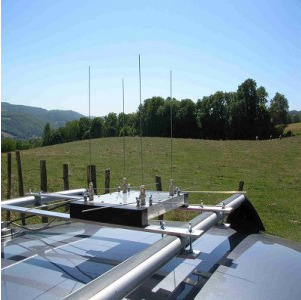
\includegraphics[height=4.2cm]{doppler}}
\logoBasGauche{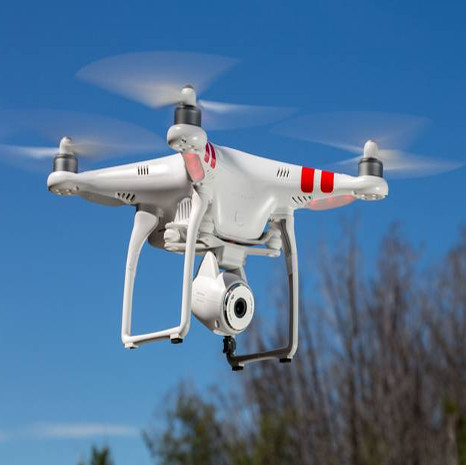
\includegraphics[height=4.2cm]{drones-quadricoptere}}
\logoBasDroit{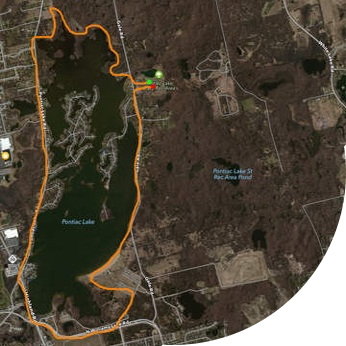
\includegraphics[height=4.2cm]{maps}}
\logoBas{
\includegraphics[height=4.2cm]{logo_ENSTA_Bretagne_Vertical_CMJN}}
\logoSmart{
\includegraphics[height=4.2cm]{Smart.png}}


%%%%%%%%%%%%%%%%%% DEBUT DU DOCUMENT
\begin{document}

\maketitle
\thispagestyle{empty}
\newpage

\tableofcontents


%%%%%%%%%%%%%%%%% INTRODUCTION


\chapter*{Résumé}
\addcontentsline{toc}{chapter}{Résumé}




Ce document présente notre rapport sur le projet SMART \og System with Multi Antennas to Reorient a Target\fg{} encadré  par M. MANSOUR Ali. Ce projet comporte deux phases: la détection d'un drone puis sa neutralisation. Compte tenu du  temps imparti nous nous sommes concentré sur la détection. De plus, nous avons choisi de réaliser notre détection avec de la radiogoniométrie, et de proposer à nos utilisateurs deux interfaces de contrôle: une application web, et une application android.


A cause de retard dans la réception de certains composants nous n'avons pas pu concevoir le capteur qui permet de détecter les drones, mais nous avons implémenté tout le système de visualisation et d'alerte, et nous avons testé au maximum les composants qui nous ont été livrés. De cet manière nous pouvons assuré que l'arrivée des quelques composants manquant suffira pour terminer ce projet. ~\\

%Ce sujet du projet vise à détecter des drones et afficher leurs positions via une application Android appelée \og S.M.A.R.T Comm Center\fg{} ou une application Web, dans le but de lutter contre les intrusions causées par les drones sur des grands centres spécifiquement nucléaires. Ce concept permet de mettre en pratique plusieurs technologies. Les méthodes et algorithmes utilisée sont inspirés du Montréal 3v2. La particularité de ce projet est qu’il vise un taux de réussite de détection pouvant atteindre 99\%. Notre projet présente un intérêt croissant pour de nombreuses entreprises. De plus, il nous a permis d’appliquer nos connaissances en télécommunication et en informatique à un domaine pratique. Toutefois, si un tel projet devait être complété, à plus ou moins longue échéance,  il serait nécessaire de tester la validité des résultats obtenus. Ainsi, on a recours à faire plusieurs tests sur le fonctionnement de différents composantes utilisées.
%Le problème le plus gênant durant la réalisation du projet est le retard dans la réception des composantes commandés(les antennes radiogoniomètres et des microcontrôleurs).~\\

% Jusqu'ici, le projet  nous a permis:
% \begin{itemize}
% \item d’appliquer la méthode radiogoniométrique
% \item d’utiliser des Raspberry PI qui permettent de transmettre les données à un ordinateur  central
% \item afficher la localisation des drones à travers une interface graphique (ordinateur central)
% \item notifier le client via une application Android.
% \end{itemize}




Nous espérons que vous prendrez autant de plaisir à lire ce rapport que nous en avons pris durant tout le déroulement de ce projet. 


\vfill{}
\textbf{Mots clés:}

Détection, drone, application Android, radiogoniomètres, application web


%%% Local Variables: 
%%% mode: latex
%%% TeX-master: "../rapport"
%%% End: 


\chapter*{Introduction}
\addcontentsline{toc}{chapter}{Introduction}

L’actualité récente a montré que l’intrusion de drones dans des sites sécurisés représentait un risque de sécurité majeur. Des gouvernements et entreprises privées se sont lancés dans la mise au point de systèmes de détection et de neutralisation de ces drones. L'équipe Smart, constituée de Rigaud Michaël, D'Acremont Antoine, Cotten Guillaume, Legay Kevin, Kenaan Aya, et Shehade Mohamed, a cherché également à répondre à cette problématique.

Mais compte tenu du temps imparti, nous avons choisi de nous concentrer dans un premier temps sur la détection d'un drone. De plus, après notre état de l'art effectué au semestre 3 nous avons choisi d'utiliser la technologie de la radio-goniométrie.  Plus exactement, nous avons choisi de réaliser la détection en plaçant un champ de radio-goniomètre. Leurs données seront transmises à un ordinateur central qui calculera la position du drone et le signalera aux utilisateurs à travers des interfaces graphiques.

Ce rapport présentera dans un premier temps un rappel de notre travail d'analyse effectué au semestre 3 ainsi que les différents tests qui ont été réalisés sur le matériel que nous avons acheté. Puis nous présenterons le travail qui a été réalisé, \cad le travail pour adapter le Montréal 3v2 à notre problème, la conception de l'interface web et l'élaboration de l'application Android. Enfin nous expliquerons comment nous avons organisé notre travail pour obtenir ce résultat, ainsi que les difficultés que nous avons rencontrées.



\newpage	  
%%%%%%%%%%%%%%%%%%%%%%%%

% \part{Etat de l'art \\(Semestre 3)}

% 
%\chapter{État de l'art des technologies}

\chapter{Présentation du contexte}

L'actualité récente a montré que l'intrusion de drones dans des sites sécurisés représentaient un risque de sécurité majeur. Des gouvernements et entreprises privées se sont lancés dans la mise au point de systèmes de détection et de neutralisation de ces drones. Une recherche bibliographique nous a permis de mettre en évidence plusieurs méthodes de détection, pouvant être classées selon trois types principaux : acoustiques, optiques et électromagnétiques.  
Les paragraphes qui suivent détailleront les différents avantages et inconvénients que ces systèmes possèdent.

\section{Acoustique}

Plusieurs entreprises proposent des outils de détection acoustique des drones. Ces derniers se présentent sous forme de boîtiers reliés à des micros, positionnés en hauteur: c'est par les sons qu'ils génèrent, principalement ceux de leurs hélices, que les drones sont repérés et cela dans un rayon d'une centaine de mètres. Certains systèmes utilisent une analyse fréquentielle poussée du signal afin de détecter les moteurs en fonction de leurs fréquences de fonctionnement. Une alerte est alors envoyée à l'utilisateur du dispositif, sur un ordinateur ou par un SMS. L'avantage principal du système est qu'il peut détecter les drones n'émettant aucun rayonnement électromagnétique comme les systèmes auto-pilotés. Au-delà de cet aspect, il présente un avantage et des plus importants, son coût. En effet, un tel système est très économique à produire. Actuellement diverses solutions actives comme passives sont déjà présentes sur le marché et la démocratisation de ce type de système tends à faire baisser leur prix.

Toutefois ces appareils présentent certains défauts qui peuvent affecter leur fiabilité. Leur efficacité est en effet dépendante du bruit de fond qui doit être inférieur à un certain seuil pour que le système puisse détecter un drone. D'autres phénomènes acoustiques comme la réverbération du son et la présence d'échos peuvent aussi perturber son fonctionnement. Cela rend l'utilisation de telles solution difficile en milieu urbain. Enfin, il est nécessaire de disposer préalablement d'une base de données des signatures acoustiques des différents drones qui peuvent émettre sur un domaine de fréquences acoustiques larges. Il est assez simple pour un drone de parer ce système de détection. Par la simple émission d'une onde sonore couvrant sa propre signature acoustique, un drone passerait totalement inaperçu.

 Ces solutions sont orientées vers une utilisation domestique et non professionnelle pour les raisons évoquées précédemment. Leur prix se situe aux alentours de 100 dollars pour un modèle simple.

\section{Optique}

Une caméra normale a besoin de lumière pour produire une image, une caméra thermique (ou infrarouge) peut capter de très faibles différences de température et les convertir en une excellente image thermique sur laquelle les plus petits détails sont visibles. Contrairement à d'autres technologies, comme l'amplification de lumière qui nécessite une petite quantité de lumière pour produire une image, l'imagerie thermique permet de voir dans l'obscurité totale. Elle ne nécessite aucune source de lumière.

Depuis qu'il est possible de produire une image lisible dans l'obscurité totale, la technologie de l'imagerie thermique permet de voir et de cibler les forces ennemies dans la nuit la plus noire. Les caméras thermiques voient à travers la brume, la pluie et la neige. Elles voient aussi à travers la fumée, ce qui était particulièrement intéressant pour l'armée.\cite{optique}

En mode passif, \emph{des caméras thermiques d'observation savent repérer un drone de 50 cm d'envergure à une distance d'environ 1 km, de jour comme de nuit} . Lorsqu'un drone entre dans son champ de vision, des algorithmes identifient son image. La forme, la couleur et la géométrie de l'objet permettent de distinguer le drone d'éventuels oiseaux et lancer une alerte, à condition qu'il n'y ait pas d'obstacle entre la caméra et lui.

En mode actif, on peut éclairer une scène à $360^{\circ}$ avec un laser. \emph{Les photons, les particules de lumière, se réfléchissent sur l'appareil, le signal est récupéré et analysé.} D'une portée similaire à celle de la caméra, le laser a l'avantage de \emph{décamoufler} (observation à travers brouillard, pluie ou filet de camouflage), de livrer la distance précise de l'objet, et de le reconstituer en imagerie 3D.Une fois le drone suffisamment proche, une caméra \textit{classique} avec un opérateur humain peuvent prendre le relai pour vérifier visuellement la nature de l'intrus et éventuellement passer à la phase de neutralisation.

L'utilisation d'un caméra optique simple pourrait aussi convenir à condition d'utiliser un traitement d'image adapté. La complexité de ce traitement associé au nombres de formes de drones pouvant être acheté dans le commerce rends cette technique difficilement exploitable.


\section{Radar}
Le radar (de l'anglais RAdio Detection And Ranging) est un système qui utilise les ondes électromagnétiques pour détecter la présence d'objets. Le radar émet des ondes, elles rebondissent sur les objets rencontrés et il est possible de mesurer leur distance, la direction, l'altitude ainsi que la vitesse en analysant le signal renvoyé. Les modèles Doppler peuvent ainsi détecter les objets en mouvement : avion, hélicoptère et certains modèles de drones, même « légers ». C'est le cas du radar Squire de Thales Air Systems. 

~\\

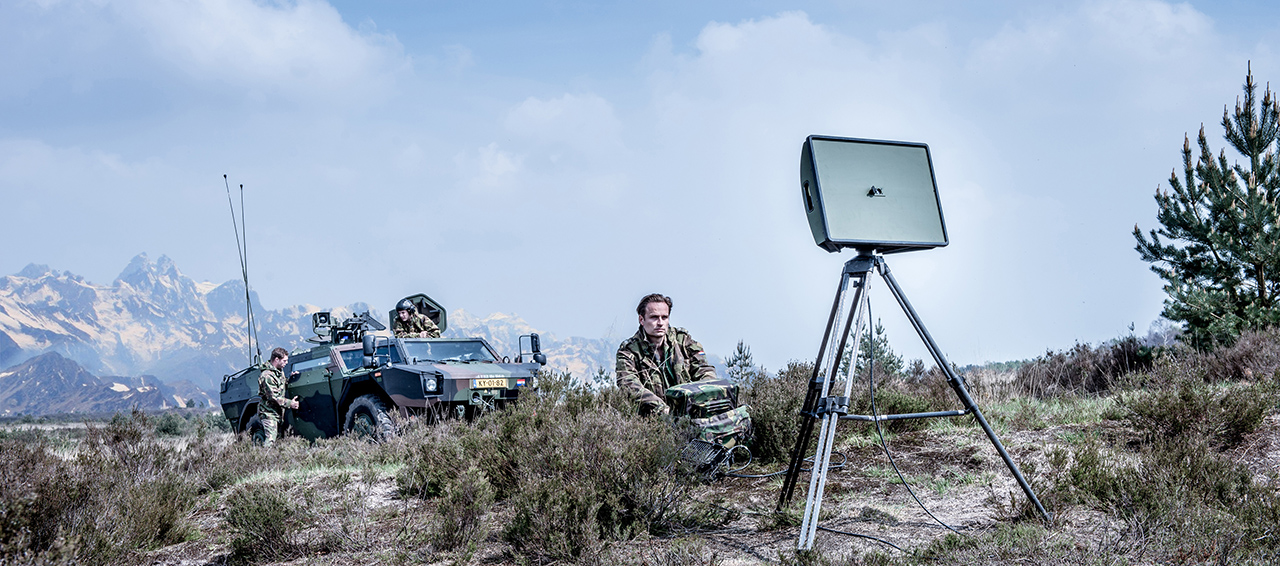
\includegraphics[width=\textwidth]{radar}
\captionof{figure}{Le radar portable Squire de Thales Air Systems}

Il existe néanmoins certains drones construits en carbone pouvant être perméables à certaines ondes radars et ainsi indétectable par cette technologie. Cependant le "radar passif", radar exploitant les variations d'ondes électromagnétiques en milieu urbain, telles que les ondes de la TNT, pourrait être exploité en milieu urbain.



\section{Radiogoniométrie}

Parmi les moyens existants pour détecter un drone on peut citer la radiogoniométrie. Le principe de la radiogoniométrie est de mesurer la direction d'arrivée d'une onde électromagnétique polarisée incidente sur un réseau de capteur, par rapport à une direction de référence. Les radio-goniomètres sont donc des détecteurs passifs. 

La radiogoniométrie possède de nombreuses applications. Cependant, en interception, la radiogoniométrie permet de localiser un émetteur inconnu soit en employant plusieurs récepteurs en des positions différentes, soit par calcul en fonction de la cinématique propre du récepteur. 

On distingue deux types de goniomètres: les goniomètres à une dimension qui n'estiment que le gisement ou l'azimut, et les goniomètres à deux dimensions qui estiment le gisement ou azimut ainsi que l'élévation. 


Dans le cas d'une détection de drones, le radio-goniomètre réalise une écoute de l'environnement avec un balayage de fréquences. Lorsque le drone émettra avec la personne qui le guide on pourra ainsi le localiser précisément.

L'avantage principal de la radiogoniométries est qu'il s'agit d'une méthode de détection passive. Elle est donc difficilement décelable et cela fait d'elle une technique fréquemment utilisée en guerre électronique. 

Seulement, la radiogoniométrie a des failles. En effet, il existe sur le marché des drones auto-pilotés qui n'émettent pas car ils chargent avant le début de leur vol leurs trajectoires. Ainsi il n'y a pas de communication avec un quelconque utilisateur, et donc il n'y a aucun signal émis. Il est donc impossible de les localiser à l'aide de cette technique.





\section{Synthèse}

Une solution technique idéal couplerait l'ensemble des méthodes décrites ci-dessus pour pouvoir parer à toute éventualité. Une analyse des solutions présentes sur le marché ou en développement montre que les configurations les plus performantes associent au moins deux des modes de détection cités. On peut notamment citer le cas du système drone-detector \cite{dronedetector}.

Néanmoins nous avons choisi pour ce projet de nous concentrer, dans un premier temps, sur une détection uniquement à base de radiogoniométrie.

Les raisons de ce choix sont les suivantes : Dans un premier temps, pour pouvoir réaliser un prototype fonctionnel il est plus aisé de se baser sur la radiogoniométrie compte tenu du matériel à notre disposition. Dans un second temps, notre équipe à choisi de se concentrer sur la détection de drones de loisir disponibles dans le commerce. Selon la réglementation ces drones doivent maintenir un lien radio avec un pilote qui doit être en mesure de reprendre le contrôle du drone à tout instant. Il y a donc une liaison permanente qui peut être exploitée par le système.




% Ici il va falloir préciser plusieurs choses sur pourquoi ce choix. Notamment en précisant qu'on suppose que les drones respectent la réglementation, etc... 



%%% Local Variables: 
%%% mode: latex
%%% TeX-master: "rapport_analyse"
%%% End: 

% \chapter{Analyse fonctionnelle}

\section{Interview}

Après notre interview avec notre encadrant Ali Mansour, nous avons réalisé un tableau des spécifications suivantes:

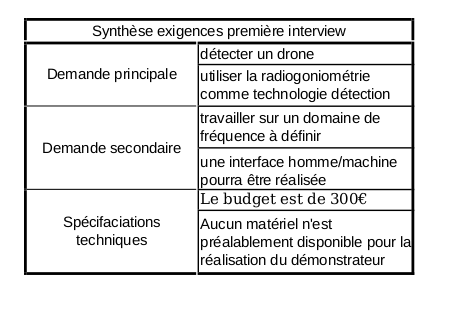
\includegraphics[width=0.8\textwidth]{interview}


\section{Tableau des spécifications}
En prenant en compte les recommandations de notre encadrant, et les recherches que nous avons réalisées, nous avons établi les contraintes et les spécifications suivantes:

%\includegraphics[width=\textwidth]{tableauSpe}
\includepdf{./images/tableauSpe.pdf}

%Compte tenu des recherches que nous avons réalisées, nous avons établi l'étude fonctionnelle suivante.

%De la synthèse de ce tableau découle le diagramme Pieuvre et les SADT suivant.

\section{Diagramme pieuvre}
~\\
~\\
~\\
~\\
~\\
~\\
\hspace{-2cm}
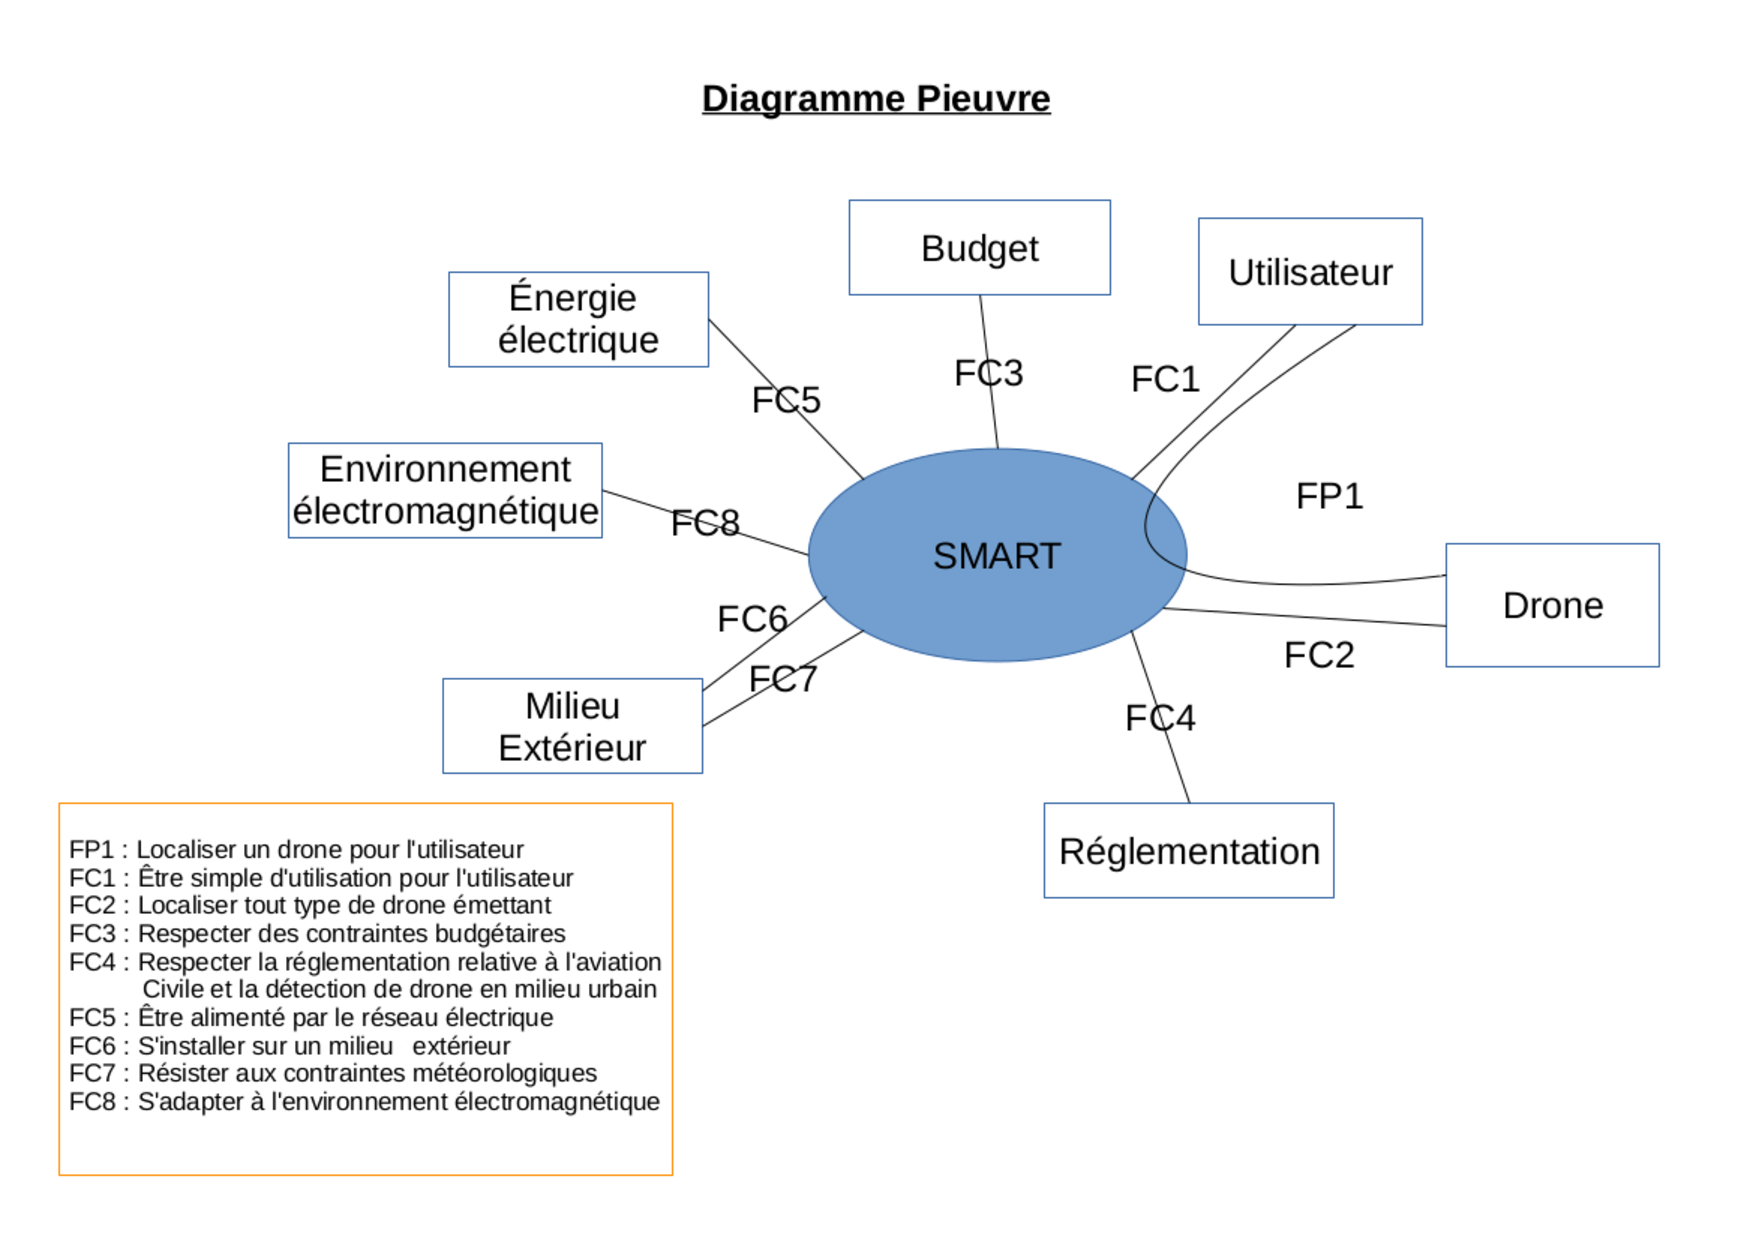
\includegraphics[width=1.18\textwidth]{Diagramme_pieuvre.pdf}
\captionof{figure}{Diagramme pieuvre}



\section{SADT}

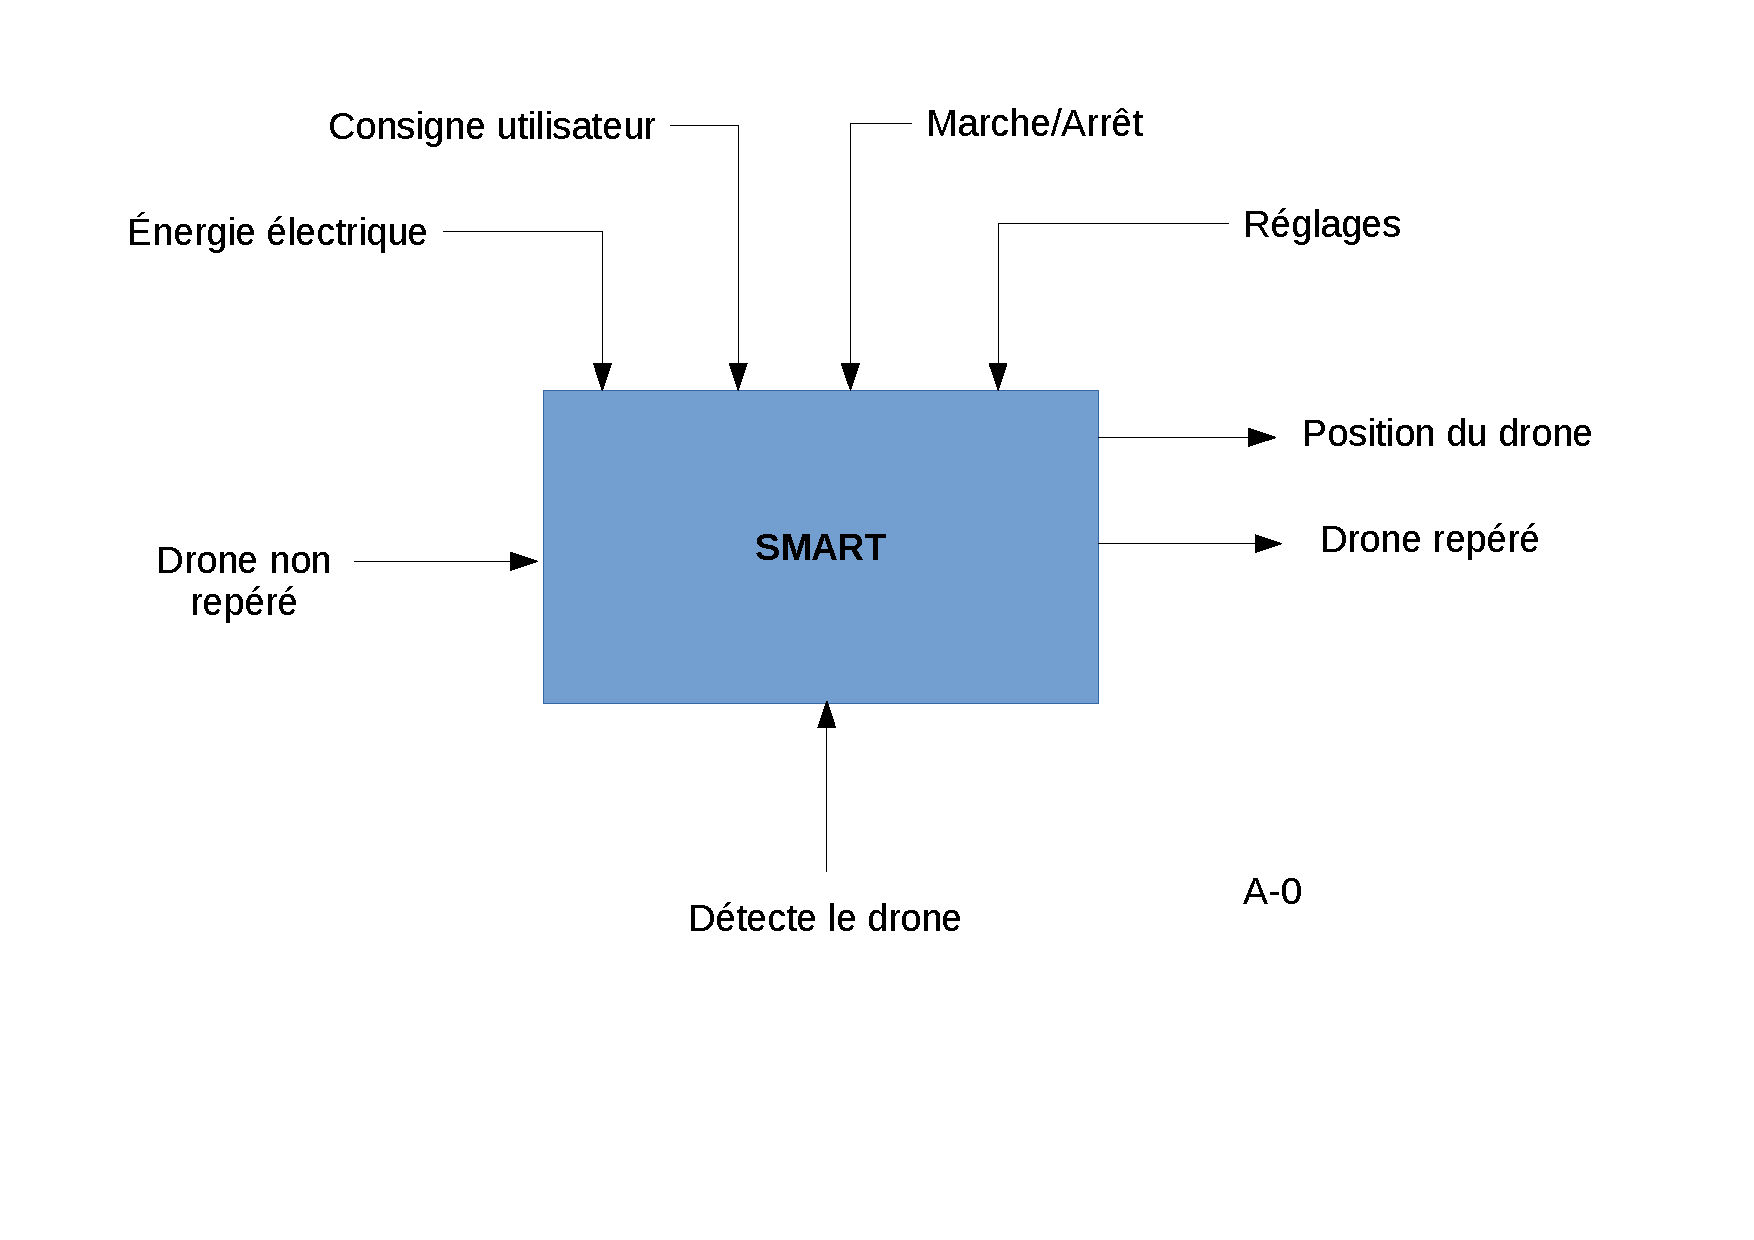
\includegraphics[width=\textwidth]{SADT_A-0.pdf}
\captionof{figure}{SADT A-0}
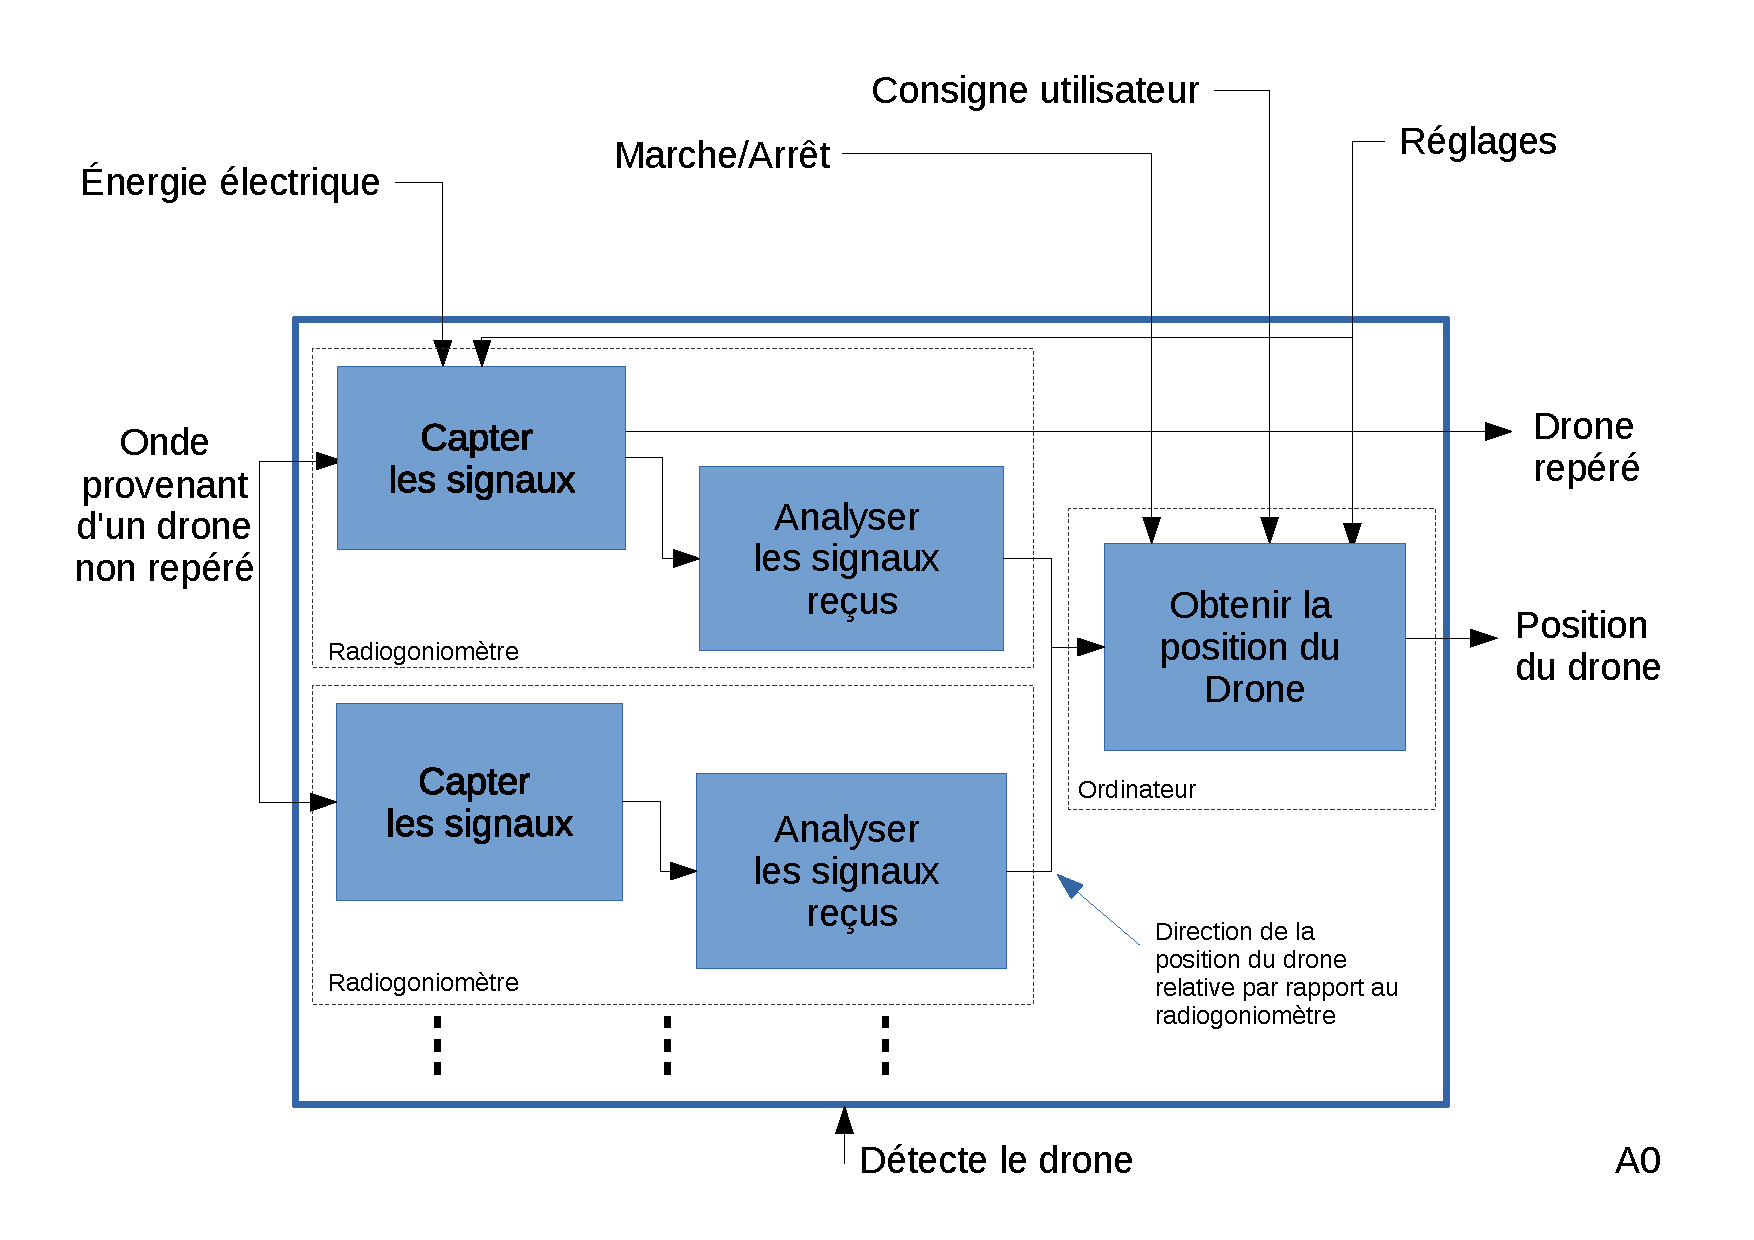
\includegraphics[width=\textwidth]{SADT_A0.pdf}
\captionof{figure}{SADT A0}

\newpage
\parindent=15pt

Comme on peut le voir sur le SADT A0, nous avons découpé notre objectif en trois parties.

Dans un premier temps il faut capter les signaux. Pour cela il faut réaliser un balayage sur le radiogoniomètre pour détecter les bons signaux.

Ensuite, il faut analyser les signaux reçus pour s'assurer que nous sommes bien en présence d'un drone.

Enfin, il faut récupérer les données des radiogoniomètres pour déterminer la position du drone.


\section{Fonctionnement de notre système}

Nous avons donc imaginé positionner plusieurs radiogoniomètres, chaque appareil indiquerait la direction du drone par rapport à sa position. Chacun d'eux serait connecté à un ordinateur central qui analyserai chacune des positions données par les radiogoniomètres et en déduirait la position du drone dans l'espace.

~\\

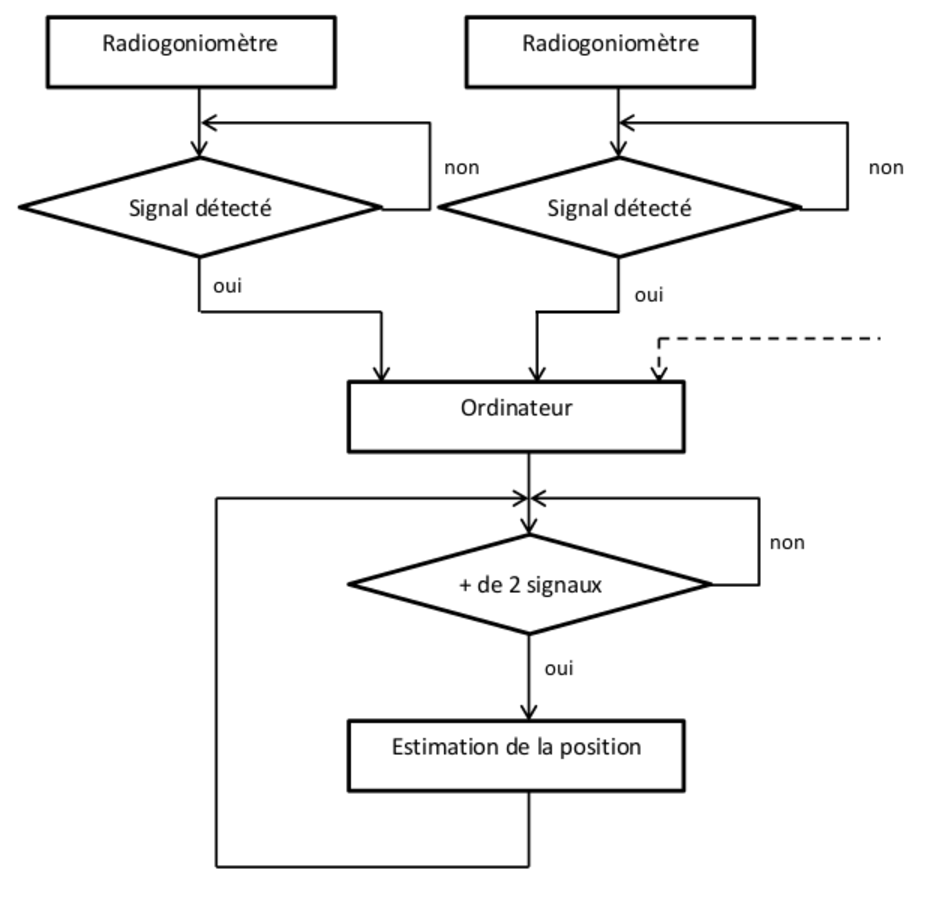
\includegraphics[width=0.8\textwidth]{SMART_logic}
\captionof{figure}{Schéma Logique du système}




%%% Local Variables: 
%%% mode: latex
%%% TeX-master: "rapport_analyse"
%%% End: 

% \chapter{Radio-goniométrie}



Dans cette partie, nous allons nous attacher à étudier les différents types de goniométrie existant afin de retenir la solution la plus pertinente pour notre système. Cette étude redéfinira dans un premier temps le cadre de l’étude, puis suivra une explication de chaque technologie existante afin de conclure sur le choix que nous aurons retenu.
~\\

Généralement, un système de radiogoniométrie est composé de  :

\begin{itemize}
\item Un réseau de N capteurs avec ou sans processus de mise en forme des signaux d’antennes.

\item Un commutateur d’antenne
\item Un récepteur à plusieurs voies
\item Une unité de traitement du signal

\end{itemize}
~\\
De plus, la composition du système d’acquisition et les techniques de traitement du signal dépendent :
\begin{itemize}
\item  Des caractéristiques de l’onde à étudier
\item  Du type d’acquisition de l’information
\end{itemize}
~\\
Dans notre application, le système devra détecter une onde émise dans la gamme de fréquence UHF (2,4 GHz). Bien qu’existant dans le domaine de réalisation des radiogoniomètres, il n’est pas commun qu’un radiogoniomètre travail sur cette gamme de fréquence.

Les caractéristiques principales qui interviennent principalement dans le choix d’un radiogoniomètre sont:

\begin{itemize}
\item La précision de mesure angulaire (précision de la position obtenue)
\item La sensibilité (portée maximale du système) 
\item La vitesse de mesure
\item Le comportement en présence de plusieurs ondes dans la bande d’analyse
\item La susceptibilité du système
\end{itemize}
~\\
La spécificité de notre système est la cible à localisé. En effet, la source peut ne pas émettre en  continue et sur de très courtes période (inférieure à 1 seconde). Il nous faut donc un radiogoniomètre capable de réalisé la mesure en une fraction de seconde. La gestion de conservation de la donnée mesurée en attendant une valeur ultérieure sera gérée par l’ordinateur.


\section{Type de goniométrie}

\subsection{Goniométrie d'amplitude}

	La mesure se fait par repérage d’un maximum d’amplitude, d’un minimum d’amplitude, ou par comparaison de d’amplitude en sortie de deux diagrammes se recouvrant partiellement. La recherche du minimum d’amplitude à partir d’une antenne à cadre tournante est l’approche la plus ancienne. Un dipôle électrique est utilisé pour lever l’ambiguïté de 180\up{o} en formant un diagramme en cardioïde par sommation.
	
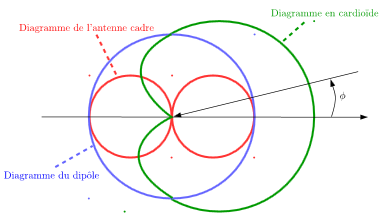
\includegraphics[width=\textwidth]{cardioide}
\captionof{figure}{diagramme en cardioide d’une antenne à cadre}
\parindent=15pt

	La formation de faisceaux est une technique plus récente issue des traitements radar. Elle utilise un ensemble de capteurs spatialement répartis. Les sorties d’antennes sont pondérées en phase puis sommées. Cette pondération est fonction du déphasage progressif d’une antenne à une autre, qui dépend de la direction d’arrivée et de la distance entre capteurs. Les pondérations permettent ainsi de remettre en phase les signaux et d’obtenir un diagramme avec un maximum dans la direction d’arrivée.
 Cette technologie est la plus ancienne. L’antenne utilisée était une antenne cadre et la gamme de fréquence étudiée était la HF et la VHF.

\subsection{Goniométrie Watson-Watt}
\label{Watson-Watt}

	Un radiogoniomètre Watson-Watt est un radiogoniomètre automatique. L’onde électromagnétique du système à localisé est reçue par deux antennes perpendiculaires dont le rapport des amplitudes est très proche de tan (l’une en sin et l’autre en cos). La goniométrie par interférométrie est considérée comme une technique plus performante comparée à celles citées précédemment. A la différence des deux techniques précédentes, le traitement n’est pas entièrement analogique. Des calculs numériques, plus ou moins complexes, sont nécessaires suivant la topologie de l’antenne utilisée. Elle n’a donc pu être mise en œuvre qu’à partir de l’arrivée des microprocesseurs.

\subsection{Goniométrie par interférométrie}

	La goniométrie par interférométrie est considérée comme une technique plus performante comparée à celles citées précédemment. A la différence des deux techniques précédentes, le traitement n’est pas entièrement analogique. Des calculs numériques, plus ou moins complexes, sont nécessaires suivant la topologie de l’antenne utilisée. Elle n’a donc pu être mise en œuvre qu’à partir de l’arrivée des microprocesseurs.
L’interférométrie utilise la mesure de la différence de phase de signaux délivrés par deux antennes proches illuminées par la même onde électromagnétique.

\subsection{Goniométrie par effet Doppler}

	Une antenne tournant autour d'un axe est placé dans le champ d'émission d'un émetteur de porteuse pure. A cause du mouvement de l'antenne, le signal reçu subit un effet Doppler qui se traduit par une modulation FM du signal reçu. La fréquence instantanée du signal augmente quand l’antenne se rapproche de la direction d’arrivée du signal et décroît lorsqu’elle s’en éloigne. En effectuant une démodulation FM, on peut détecter la direction de provenance des ondes en comparant la phase du signal obtenu et celle de la rotation angulaire de l’antenne. 
Afin d'éviter de devoir faire tourner mécaniquement l'antenne, on peut en disposer plusieurs en cercle et les commuter successivement.

\section{Selection de la technologie}

	Après étude des différentes technologies existantes, nous nous baserons sur une étude comparative menée par le site F1LVT.

~\\	
	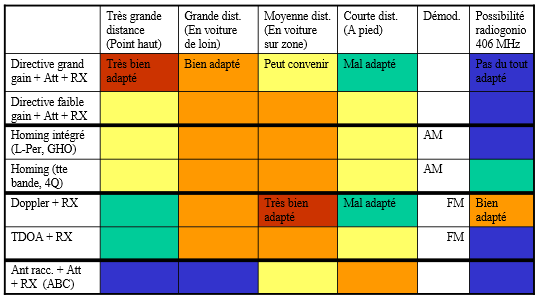
\includegraphics[width=\textwidth]{tableauTechnologies}
	\captionof{figure}{Radiogoniométrie VHF-UHF pour les bandes aviation et les bandes RA}
\parindent=15pt
~\\

	Ce tableau compare plusieurs technologies ainsi que leurs caractéristiques. Dans le cadre d’un système devant opéré en extérieur sur zone (environ de zone industriel ou de central électrique ) nous retenons le goniomètre Doppler.





%%% Local Variables: 
%%% mode: latex
%%% TeX-master: "rapport_analyse"
%%% End:

% \chapter{Composants}


\section{Antennes}

\subsubsection{Principes généraux}

	Les goniomètres utilisent les ondes radioélectriques pour pouvoir localiser la direction d'une source d'émissions. Chaque type de goniomètre utilisera une ou plusieurs antennes pour pouvoir analyser les caractéristiques de l'onde reçue. 
	Le fonctionnement de ces antennes est décrit par les lois de l'électromagnétisme. Chaque onde électromagnétique possède une composante électrique et une composante magnétique. La composante ou champ électrique de cette onde fera apparaitre des variations de potentiel dans l'antenne dont l'amplitude et la fréquence seront directement liés à l'onde qui les a généré. Leur analyse permettra de récupérer les caractéristiques de l'onde reçue et d'en extraire les informations pertinentes pour le système équipé de l'antenne.
	
\subsection{Antennes en Radiogoniométrie}

	En radiogoniométrie il est possible de travailler avec plusieurs types d'antennes. La méthode la plus simple pour déterminer la direction d'une onde sera d'utiliser une antenne à ouverture dite faible et de la faire pivoter pour pouvoir déterminer la direction du maximum d'émission. Une antenne circulaire ou rectangulaire pourra convenir. Parfois le type de goniomètre utilisé déterminera le choix de l'antenne. Par exemple dans le cas d'un radiogoniomètre de type Watson-Watt plusieurs solutions sont envisageables: 
	
\begin{itemize}

\item l'utilisation de deux antennes circulaires ou rectangulaires.

\item L'utilisation d'une antenne dite "Adcock" qui est une combinaison d'antennes monopoles ou dipolaires. 

\end{itemize} 

	Dans le cadre de notre projet, nos recherches nous ont conduit à choisir un goniomètre Doppler. Ce type de goniomètre utilise au minimum quatres antennes monopoles ou dipolaires disposées en croix autour d'une antennes de référence omnidirectionnelle (une antenne monopole est souvent utilisée). Pour un nombre d'antennes supérieur celles-ci seront disposées en cercle à intervalle régulier autour de l'antenne de référence.	
	
	En théorie deux antennes pourraient suffire. Si on parvenait à mettre en rotation une antenne omnidirectionelle autour de l'antenne de référence suffisamment rapidement le goniomètre Doppler fonctionnerait. Il est toutefois beaucoup plus simple d'utiliser un ensemble d'antennes disposées en cercle et "d'écouter" successivement chaque antenne à l'aide d'un commutateur pour simuler cette rotation.
	
\subsection{Système d'antennes retenu}

	Le goniomètre Montréal possède cinq antennes, quatre disposées en croix et une antenne centrale connectées au système électronique de traitement. Les antennes sont reliées à un commutateur permettant de sélectionner successivement les antennes de la croix. Le système est dimensionné autour de trois critères : 
	
\begin{itemize}

\item La bande de fréquence surveillée par les antennes : On utilisera ici des antennes monopoles (quart d'onde) adaptées au 2,4GHz

\item Le rayon d'écartement des antennes (distance entre les quatres antennes de la croix et l'antenne de référence) : Si ce rayon est trop faible les écarte de fréquence seront plus difficiles à remarquer et le bruit électromagnétique peut être plus gênant lors de la mesure.


\item La vitesse de commutation des antennes.

\end{itemize}

Deux des paramètres sont fixés à l'installation du dispositif. Les formules suivantes permettent de déterminer le paramètre manquant.

\begin{equation}
dF = \frac{w*r*f_c}{c}
\end{equation}

et

\begin{equation}
f_r = \frac{dF*1879.8}{R*f_c}
\end{equation}

Les antennes utilisées pour le montage pourront être celles utilisées dans l'aéromodélisme et sur les drones amateurs qui utilisent dans leur grande majorité la bande des 2,4 GHz.

Les modèles d'antennes suivants pourraient convenir :

\begin{itemize}

\item FrSky 2.4G V8 Series 5db module Antenna

\item Orange 2.4G Antenna 2db (Extended wire)

\end{itemize}

Il est aussi possible de les concevoir nous même en respectant les dimensions ( 3,125 cm pour une monopole, 6.25 cm pour une dipôle)

%%% Local Variables: 
%%% mode: latex
%%% TeX-master: "rapport_analyse"
%%% End:

% \chapter{Le Montréal 3V2}
\label{montreal}

Nous allons ici présenter la solution sur laquelle nous nous appuyons pour réaliser notre propre radiogoniomètre à effet Doppler, le Montréal 3V2.
Pour réaliser cette documentation nous nous sommes appuyé sur la documentation trouvé sur le site f1lvt \cite{montreal}

\section{Évolution du Montréal}

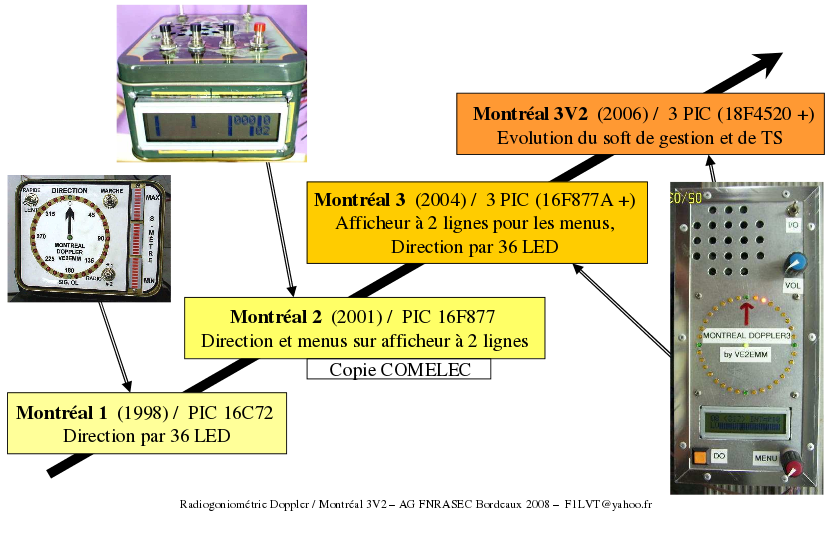
\includegraphics[width=\textwidth]{evolution}
\captionof{figure}{Evolution du Montréal}

\section{Avantages du Montréal 3v2}

\begin{center}
  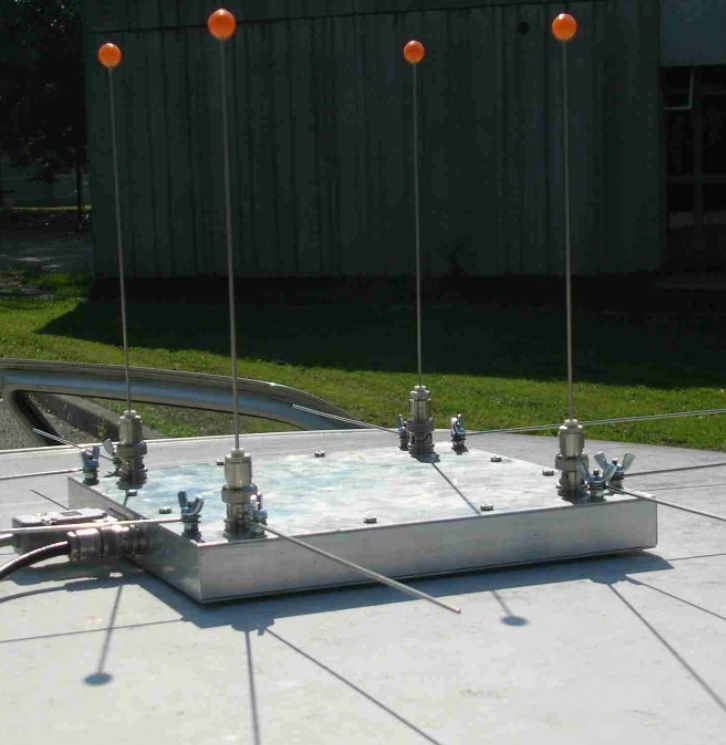
\includegraphics[width=0.5\textwidth]{montreal}
  \captionof{figure}{Photographie prise du Montréal 3v2}
\end{center}

\parindent=15pt
Le Montréal 3v2 sert principalement à l'FNRASEC\footnote{Fédération Nationale des Radioamateurs au service de la Sécurité Civile, agrée de sécurité civile} et aux chasseurs d'onde amateurs. Ce radiogoniomètre est utilisé pour la détection de balise de détresse de 406MHz.

%Parmi ses avantages, on peut noter qu'il est facile à construire, son prix , et il est simple d'utilisation. 

Un des intérêts majeurs du Montréal 3-V2, c'est sa capacité de localiser des signaux très courts, son prix de revient est très raisonnable,son traitement très rapide et la mise en mémoire automatique du dernier relevé. On peu aussi noter qu'il est simple d'utilisation grâce a son affichage à 36LED disposé en cercle et qui indique la direction. De plus une LED centrale est indique le fonctionnement; verte la direction affichée est bonne, rouge le signal est insuffisant, la direction reste alors figée dans la dernière bonne direction reçue.

%on peut noter son affichage à 36 LED qui indique la direction de manière clair et efficace, et un réglage facilité par son écran LCD ou encore son filtre à capa commutée à très faible largeur de bande (0,5 Hz).

\section{Caractéristiques}

Le Montréal 3v2 est un radiogoniomètre à effet Doppler, il possède donc toutes les caractéristiques associé a ce type de radiogoniomètre.
~\\

\begin{tabular}{ l l l}
Fréquences & distance & moyenne portée\\
 & gamme & 50MHz-1.3GHz\\
 & démodulation & FM\\
Affichage & LED & 36LED\\
& écran & LCD en 2 lignes\\
Filtre & capa & très faible largeur de bande (0.5Hz)\\
Coût & & estimé à 50\euro \\
\end{tabular}


\section{Fonctionnement}
La partie centrale contient les circuits d'amplification et de commutation. Les 4 brins verticaux (les brins actifs) se fixent par BNC.

Les antennes sont alimentées de façon séquentielle pour imiter une antenne en rotation. Une fois que les antennes ont capté les ondes provenant du drone, il faut faire une démodulation et enlever tous les bruits.


Un système à LED permet de visualiser la composante continue qui passe dans les antennes. A partir du boîtier Doppler et de son menu de test, on peut ainsi vérifier individuellement chaque antenne. Ceci permet soit de faire fonctionner le système Doppler avec une antenne sur 4 %(fonctionnement conforme à la théorie avec une seule antenne tournante)
, soit avec 3 antennes sur 4. %(ce qui inverse le signal Doppler à 500 Hz ; mais ça fonctionne aussi bien voire mieux).


Trois microcontrôleurs Pics sont utilisés un 16F628A pour l'affichage, un 16F877A pour le circuit principal et un 12F675 comme diviseur de fréquence.

Ce Doppler est la version la plus récente et la plus performante de la série. Il commute les antennes et il affiche la direction mesurée sur la boussole à 36 LED. 
~\\

Une présentation plus détaillé du fonctionnement interne des PIC est fournie dans la figure suivante:


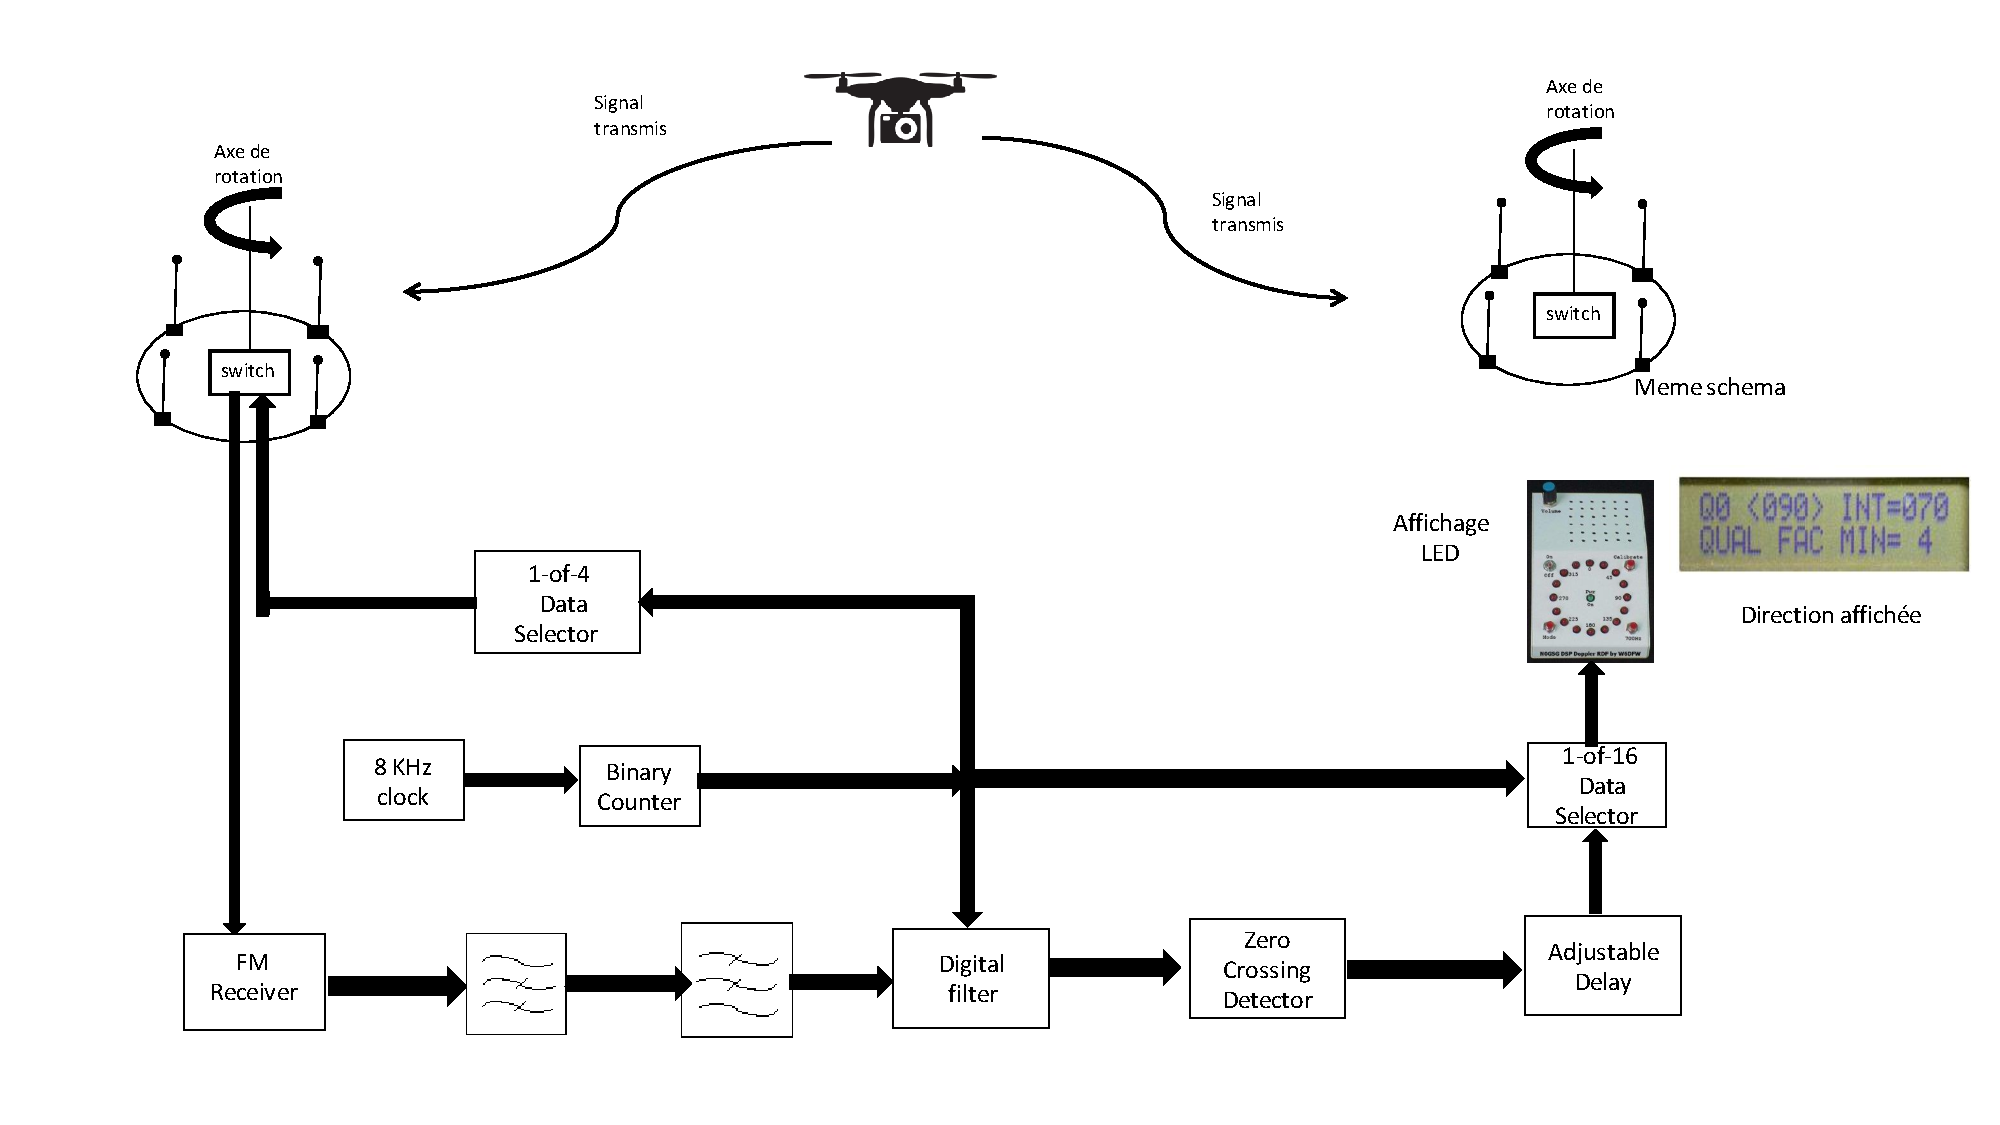
\includegraphics[width=\textwidth]{Presentation1}
\captionof{figure}{Présentation détaillé du système}



\section{Schéma bloc}

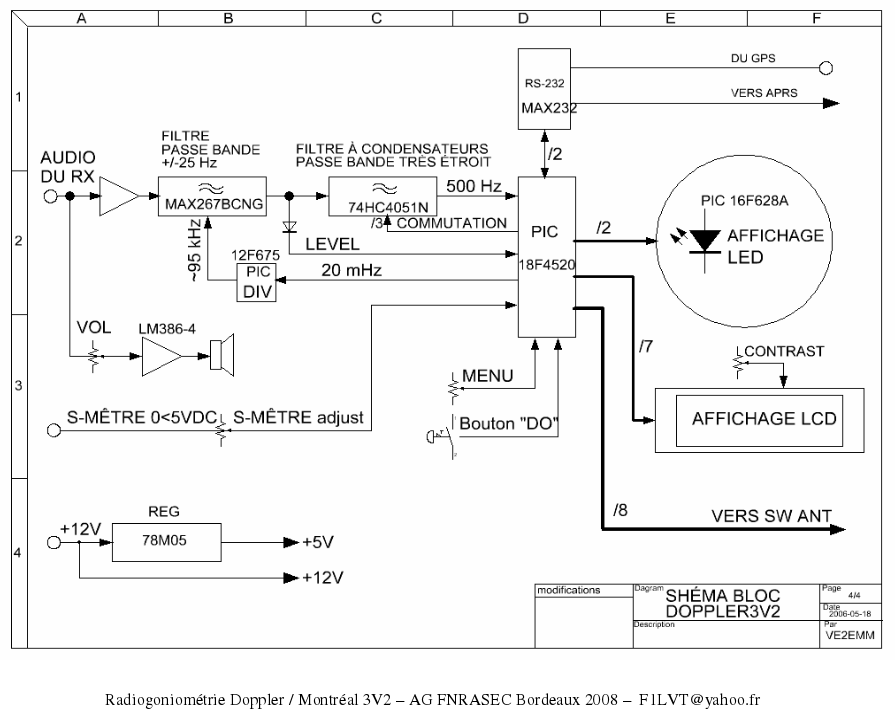
\includegraphics[width=\textwidth]{schemaBloc}
\captionof{figure}{Schéma bloc du Montréal 3v2}

\section{Liste des composants}
Voici la liste des composants pour la construction du Montréal 3v2:

\begin{tabular}{ l l l}

IC30&          LM386N-4&                  Ampli BF\\
IC50&          MAX267BCNG&          Filtre\\
IC51& PIC  12F675-I/P& PIC \\
IC52&          74HC4051N&               Filtre\\
IC53&          MAX492CPA &            Ampli Op\\
IC70& PIC  18F4520-I/P& PIC\\
VR20 &       7805 TO-220  &            Régulateur\\
X70&           20 MHz  HC49&           Quartz\\
D50&           1N5819       &                Diode Schottky\\
LCD20&      LCD 2X16,&                 Afficheur 2 lignes de 16 car.\\
IC1& PIC16F628A-I/P& PIC\\
LED1 - LED36& ø3mm, Rouge et/ou Vert&\\
LED37&                        3 ou 5mm Bicolore Rouge/Verte &\\
FB1 - FB8&                   Ferrites\footnote{+ composants passifs : Résistances, Condensateurs.}&\\
IC100&        = MAX232ACPE&        en option\\
Q100 &        = 2N2222 TO-92&\\
\end{tabular}
\captionof{figure}{Liste des composants}


%%% Local Variables: 
%%% mode: latex
%%% TeX-master: "rapport_analyse"
%%% End: 


%
\chapter{Contexte}

\section{Nature du besoin}

Les drones sont de plus en plus présents dans le monde moderne est font maintenant partie intégrante du paysage urbains. Il est en effet possible d'acheter pour 50\euro~  un drone miniature dans n'importe quel rayon de jouet de grandes surfaces comme Leclerc, Carefour, Géant Casino, ... %Mais son usage ne s'arrête pas au loisir, de grandes firmes américaines comme Amazon souhaite utiliser ces drones pour livrer leur produit
Mais son usage ne s'arrête pas au loisir puisque l'actualité a montré que l'intrusion de drones dans des sites sécurisés représentaient un risque de sécurité majeur.

Notre projet au nom de SMART (System with Multi Antennas to Reorient a Target) doit répondre a ce problème en proposant une solution de détection de drone. Pour cela nous allons utiliser un système passif qui réceptionne les ondes émises par le drone puis utilise l'effet Doppler sur ces ondes pour obtenir la direction d'émission. Ainsi grâce a deux dispositif il sera possible d'obtenir la position du drone a détecter. 




%%% Local Variables: 
%%% mode: latex
%%% TeX-master: "../rapport"
%%% End: 

%\chapter{Ingénierie Système}

\section{Analyse Fonctionelle}

\subsection{Diagramme Pieuvre}

Le diagramme pieuvre permet de mettre en évidence rapidement la fonction principale du système et les principales contraintes qui s'appliquent sur le système. Ce dernier est représenté par l'ovale central et l'ensemble des éléments extérieurs ayant une influence sont matérialisés tout autour. Les différentes relations sont appelées les fonctions de contraintes qui naissent d'une contrainte imposée par un élément extérieur « météo », de l'existence d'un produit déjà existant « un autre drone émettant des ondes » ou encore d'une exigence particulière de l'utilisateur voire de la présence de normes et de législations, de limitations lié au budget ou du type d'alimentation énergétique nécessaire.


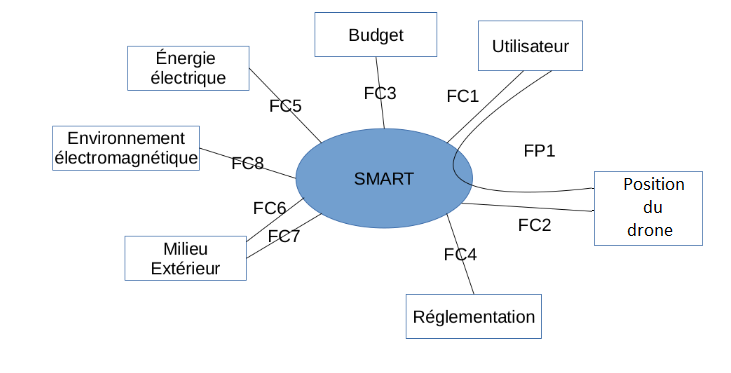
\includegraphics[width=0.90\textwidth]{Diagramme_pieuvre_corr.png}
\captionof{figure}{Diagramme pieuvre}


\subsection{Diagramme FAST}

Ce diagramme  présente la  manière de penser et d'agir. Le diagramme FAST se construit de gauche à droite, dans une logique du pourquoi au comment. On développe les fonctions de service du système en fonctions techniques. On choisit des solutions pour construire finalement notre système. On a mentionné les fonctions techniques chacune  à part pour trouver la solution convenable qui nous permet à la fin la réalisation finale du système. En utilisant des outils et méthodes déjà existant, on a trouvé des solutions qui satisfont les fonctions demandés.
L’antenne goniomètre était l’une des solutions les moins chères pour la détection du drone, à condition d’avoir au minimum deux antennes pour préciser la position et la vitesse du drone. Dès la détection du drone, il sera alors possible de déterminer sa position, d'enregistrer cette position via un logiciel dédié (MATLAB)

~\\

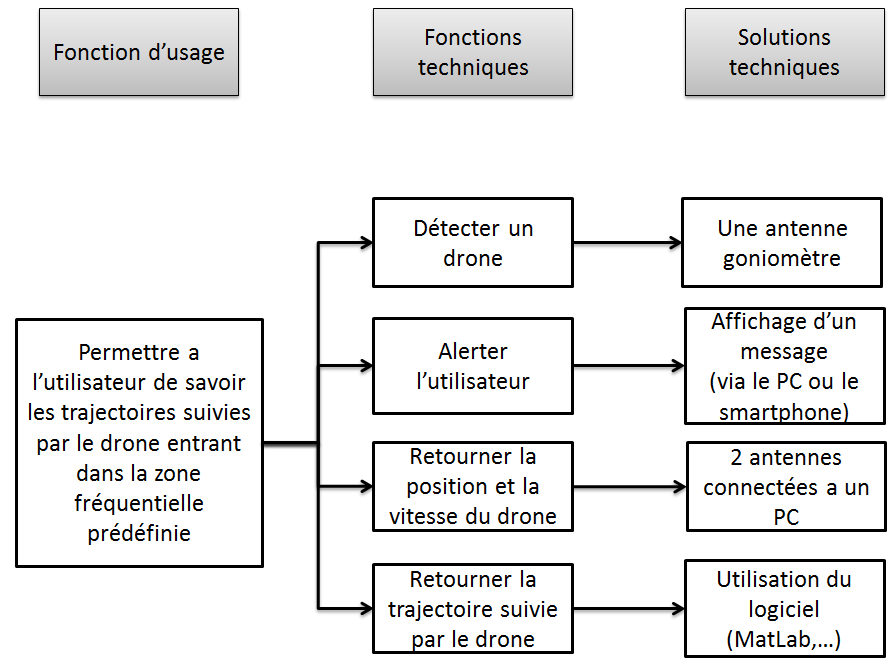
\includegraphics[width=1\textwidth]{FAST.png}
\captionof{figure}{Diagramme pieuvre}

%%% Local Variables: 
%%% mode: latex
%%% TeX-master: "../rapport"
%%% End: 

% \part{Conception de Smart \\(Semestre 4)}

\part{Préparation}



\chapter{Choix technologique}
\label{chap:choix}

\section{Rappel de notre projet}

Suite à notre état de l'art, nous avons décidé de réaliser notre système de détection en installant un maillage de capteur qui se baseront sur le système du Montréal 3V2. Chaque capteur sera connecté à un \rpi 2 \footnote{La documentation technique du Raspberry PI est situé en annexe à la page \pageref{annexe:rpi}}. De plus, chaque \rpi communiquera avec un ordinateur central qui traitera les données pour les afficher sur une interface graphique. Les données qui seront transmises sont: le numéro du \rpi, la position du capteur, et le gisement du drone par rapport au capteur. Enfin, l'ordinateur central communiquera avec une application android qui notifiera le client de la présence d'un drone comme on peut le voir sur la figure \ref{fig:inst}.
~\\

L'architecture physique du système est présenté à la figure \ref{fig:arch_phys}.

\begin{figure}[!h]
  \centering
  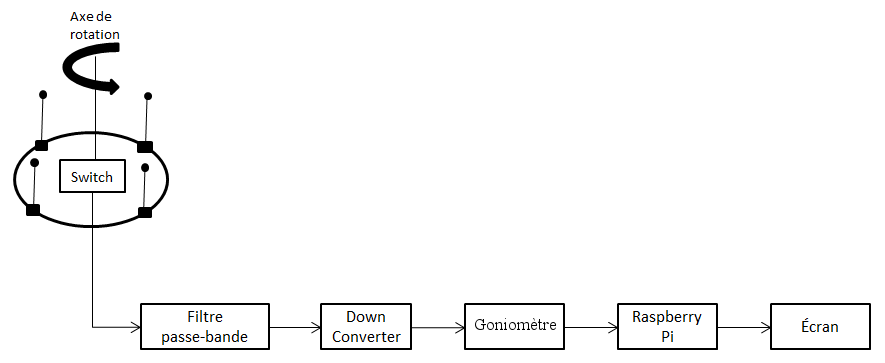
\includegraphics[width=\textwidth]{fonctionnement}
  \caption{Architecture Physique}
  \label{fig:arch_phys}
\end{figure}


\begin{figure}[!h]
  \centering
  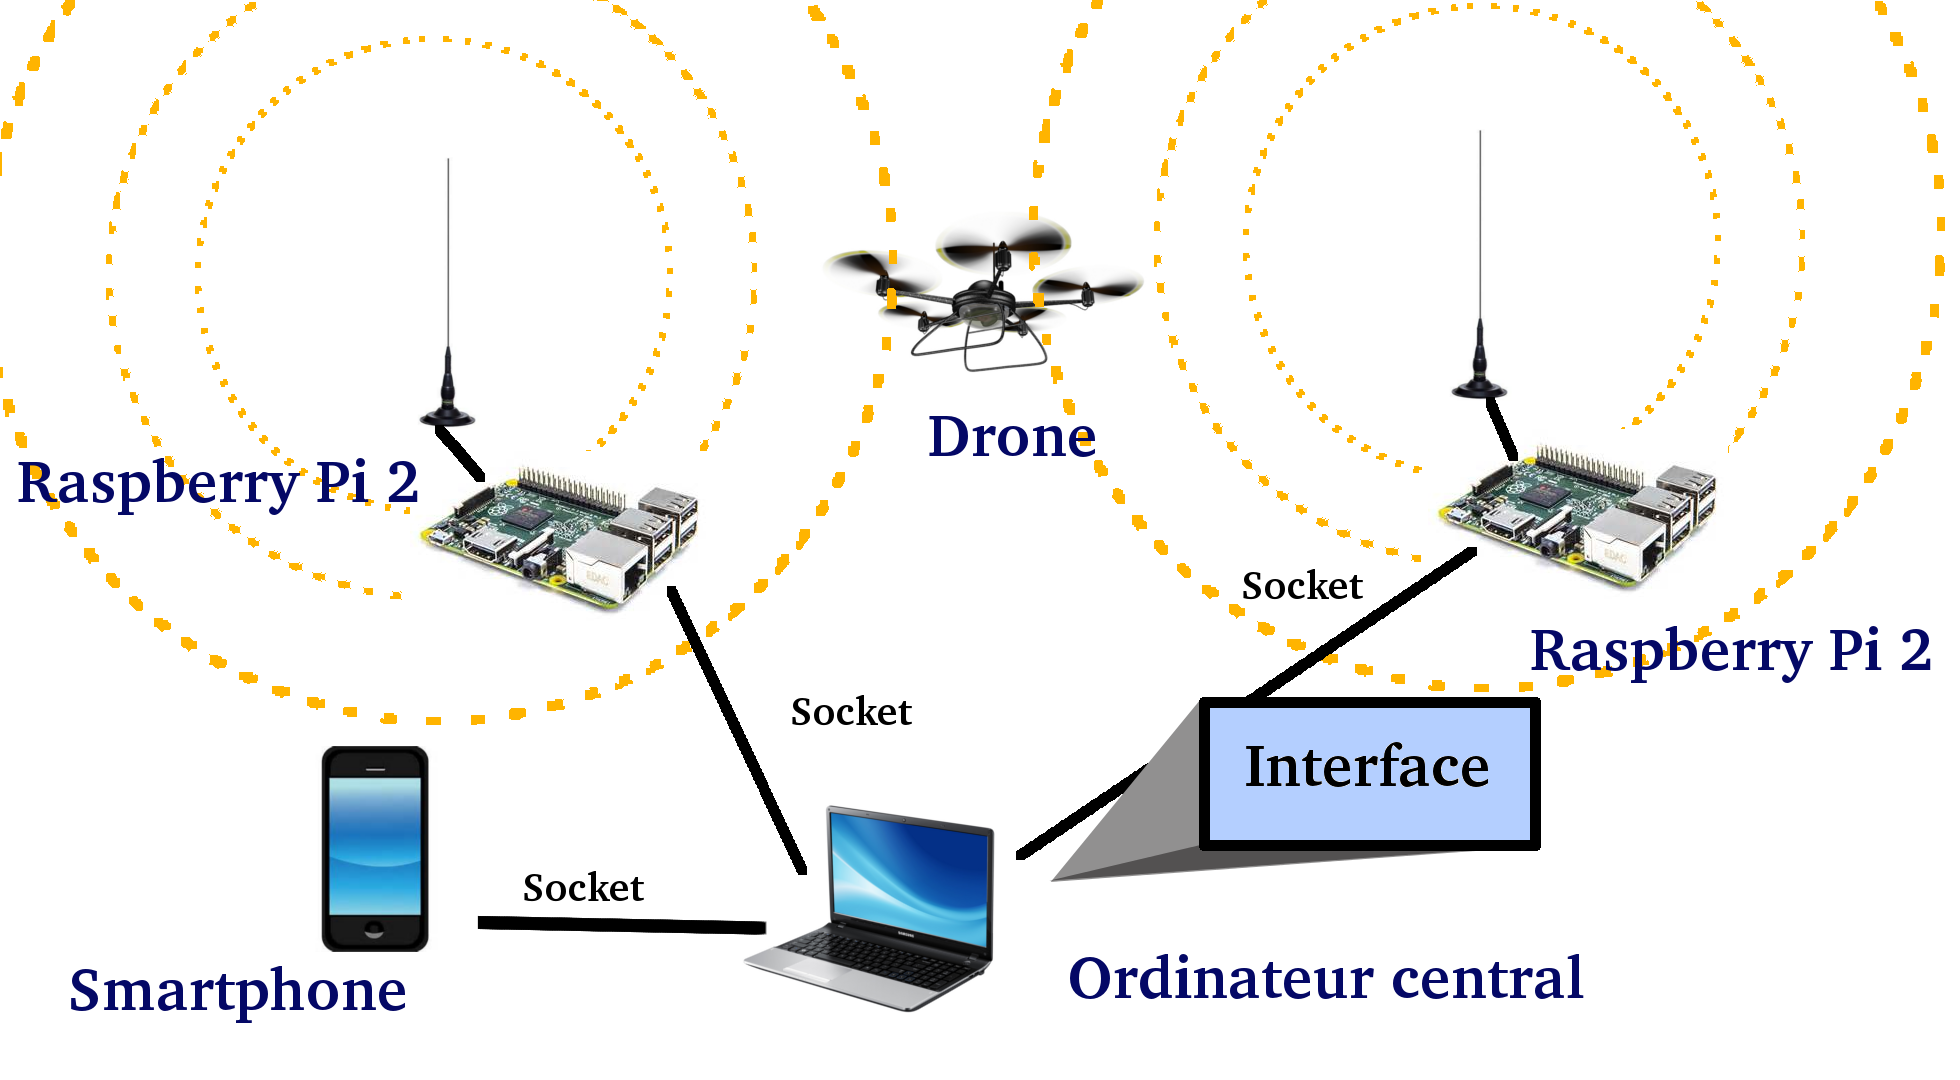
\includegraphics[width=\textwidth]{installation}
  \caption{Installation de Smart}
  \label{fig:inst}
\end{figure}




%%% Local Variables: 
%%% mode: latex
%%% TeX-master: "../rapport"
%%% End: 

\chapter{Tests unitaires}

Suite au choix que nous avons réalisé dans la partie précédente, nous avons commandé notre matériel. Dès la réception de celui-ci nous avons effectué des tests unitaires pour vérifier leur bon fonctionnement.

\section{Raspberry Pi}
La documentation technique lié a notre Raspberry Pi es situé en annexe à la page \pageref{annexe:rpi}
~\\

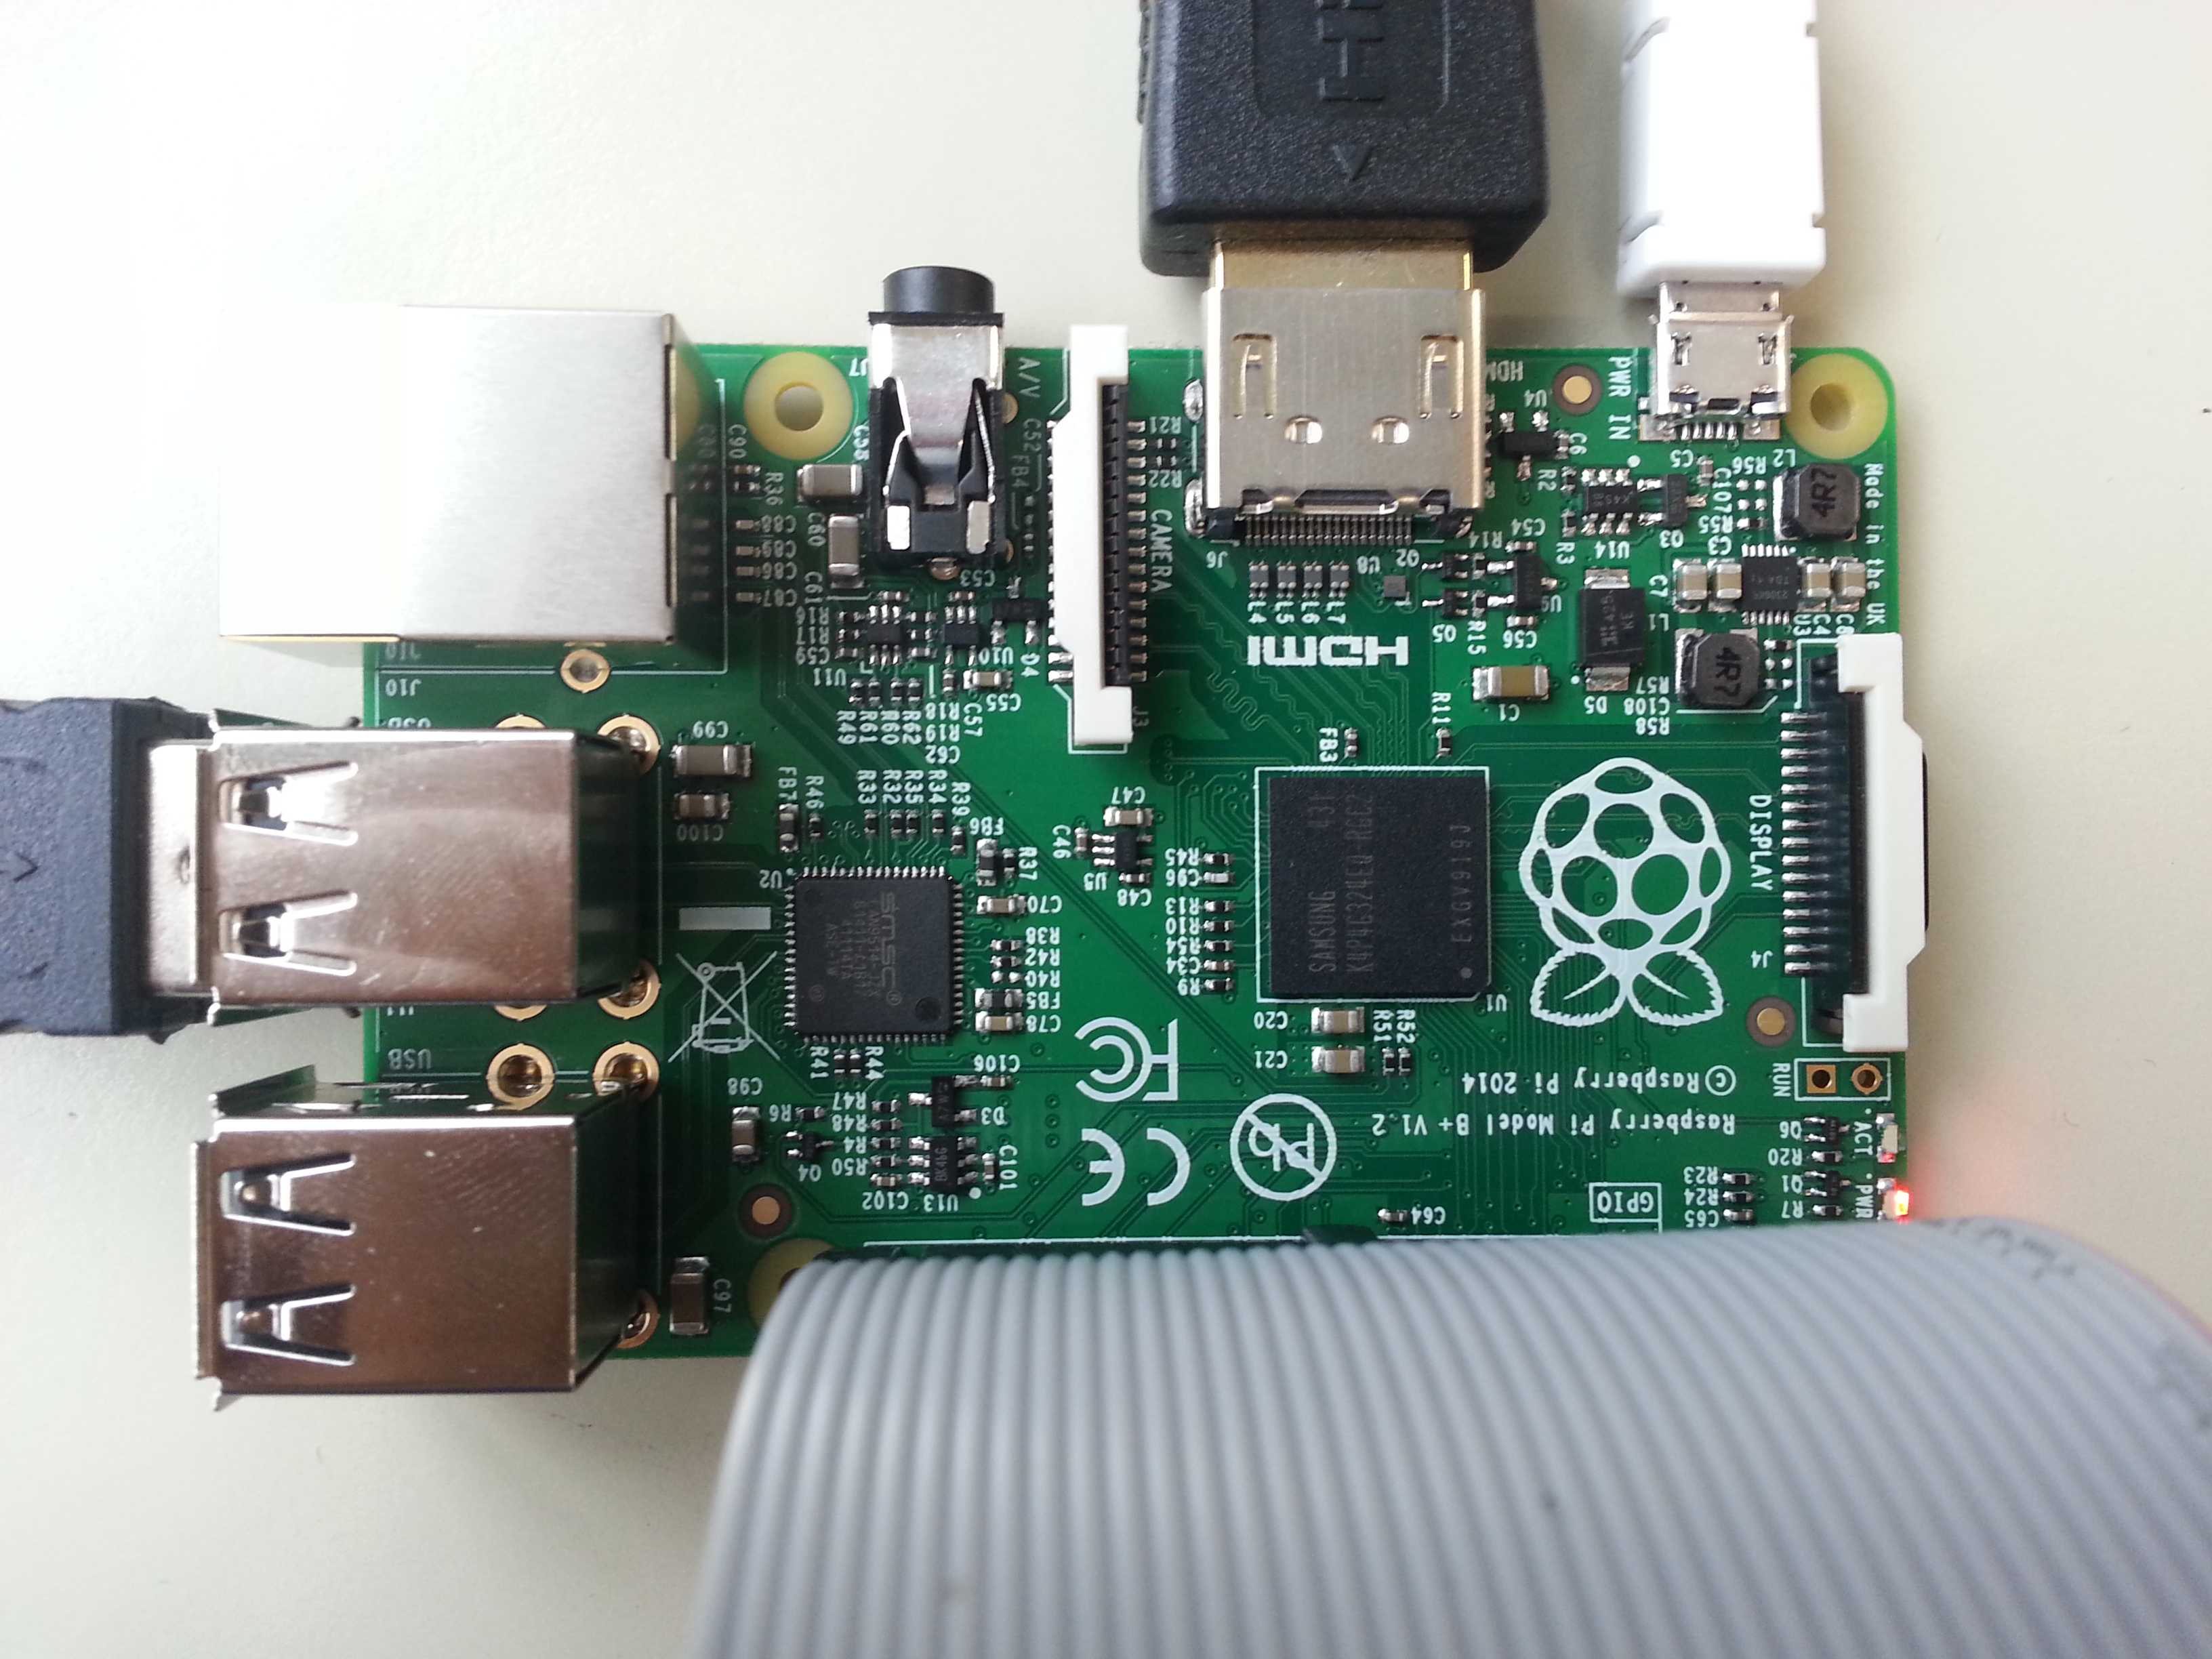
\includegraphics[width=\textwidth]{Test_unitaire/Rpi/img5.jpg}
\captionof{figure}{Notre Raspberry Pi B+}

~\\
\parindent=15pt

Pour s'assurer que notre Raspberry Pi répond aux spécifications fonctionnelles et qu'il fonctionne correctement en toutes circonstances pour notre projet, nous y avons réalisé des tests unitaires.

Après avoir enfin installé le système d'exploitation Raspbian\footnote{La documentation lié à Raspbian est situé en annexe à la page \pageref{annexe:raspbian}} sur notre Raspberry Pi B+, nous avons tenté de tester les ports GPIO. Pour cela, dans un premier temps, nous avons allumé des LED grâce à un script python à travers différents ports GPIO. Sur la figure \ref{figure:led}, on peut observer que nous avons allumé une LED grâce au port 22.
~\\

Dans notre projet le Raspberry Pi sera placé entre le radio-goniomètre à effet Doppler et l'utilisateur. Il aura deux taches, corréler les données entre tous les dispositifs pour obtenir la position du drone et afficher le résultat à l'utilisateur. Pour cela il doit récupérer la direction qui est donné par le Montréal 3v2. Cette position est donnée à travers des LED (voir figure \ref{figure:ledMontreal}). Nous allons donc placer le Raspberry Pi au niveau des LED pour obtenir les informations délivré par le Montréal 3v2. % TODO : A FINIR

\begin{figure}[!h]
  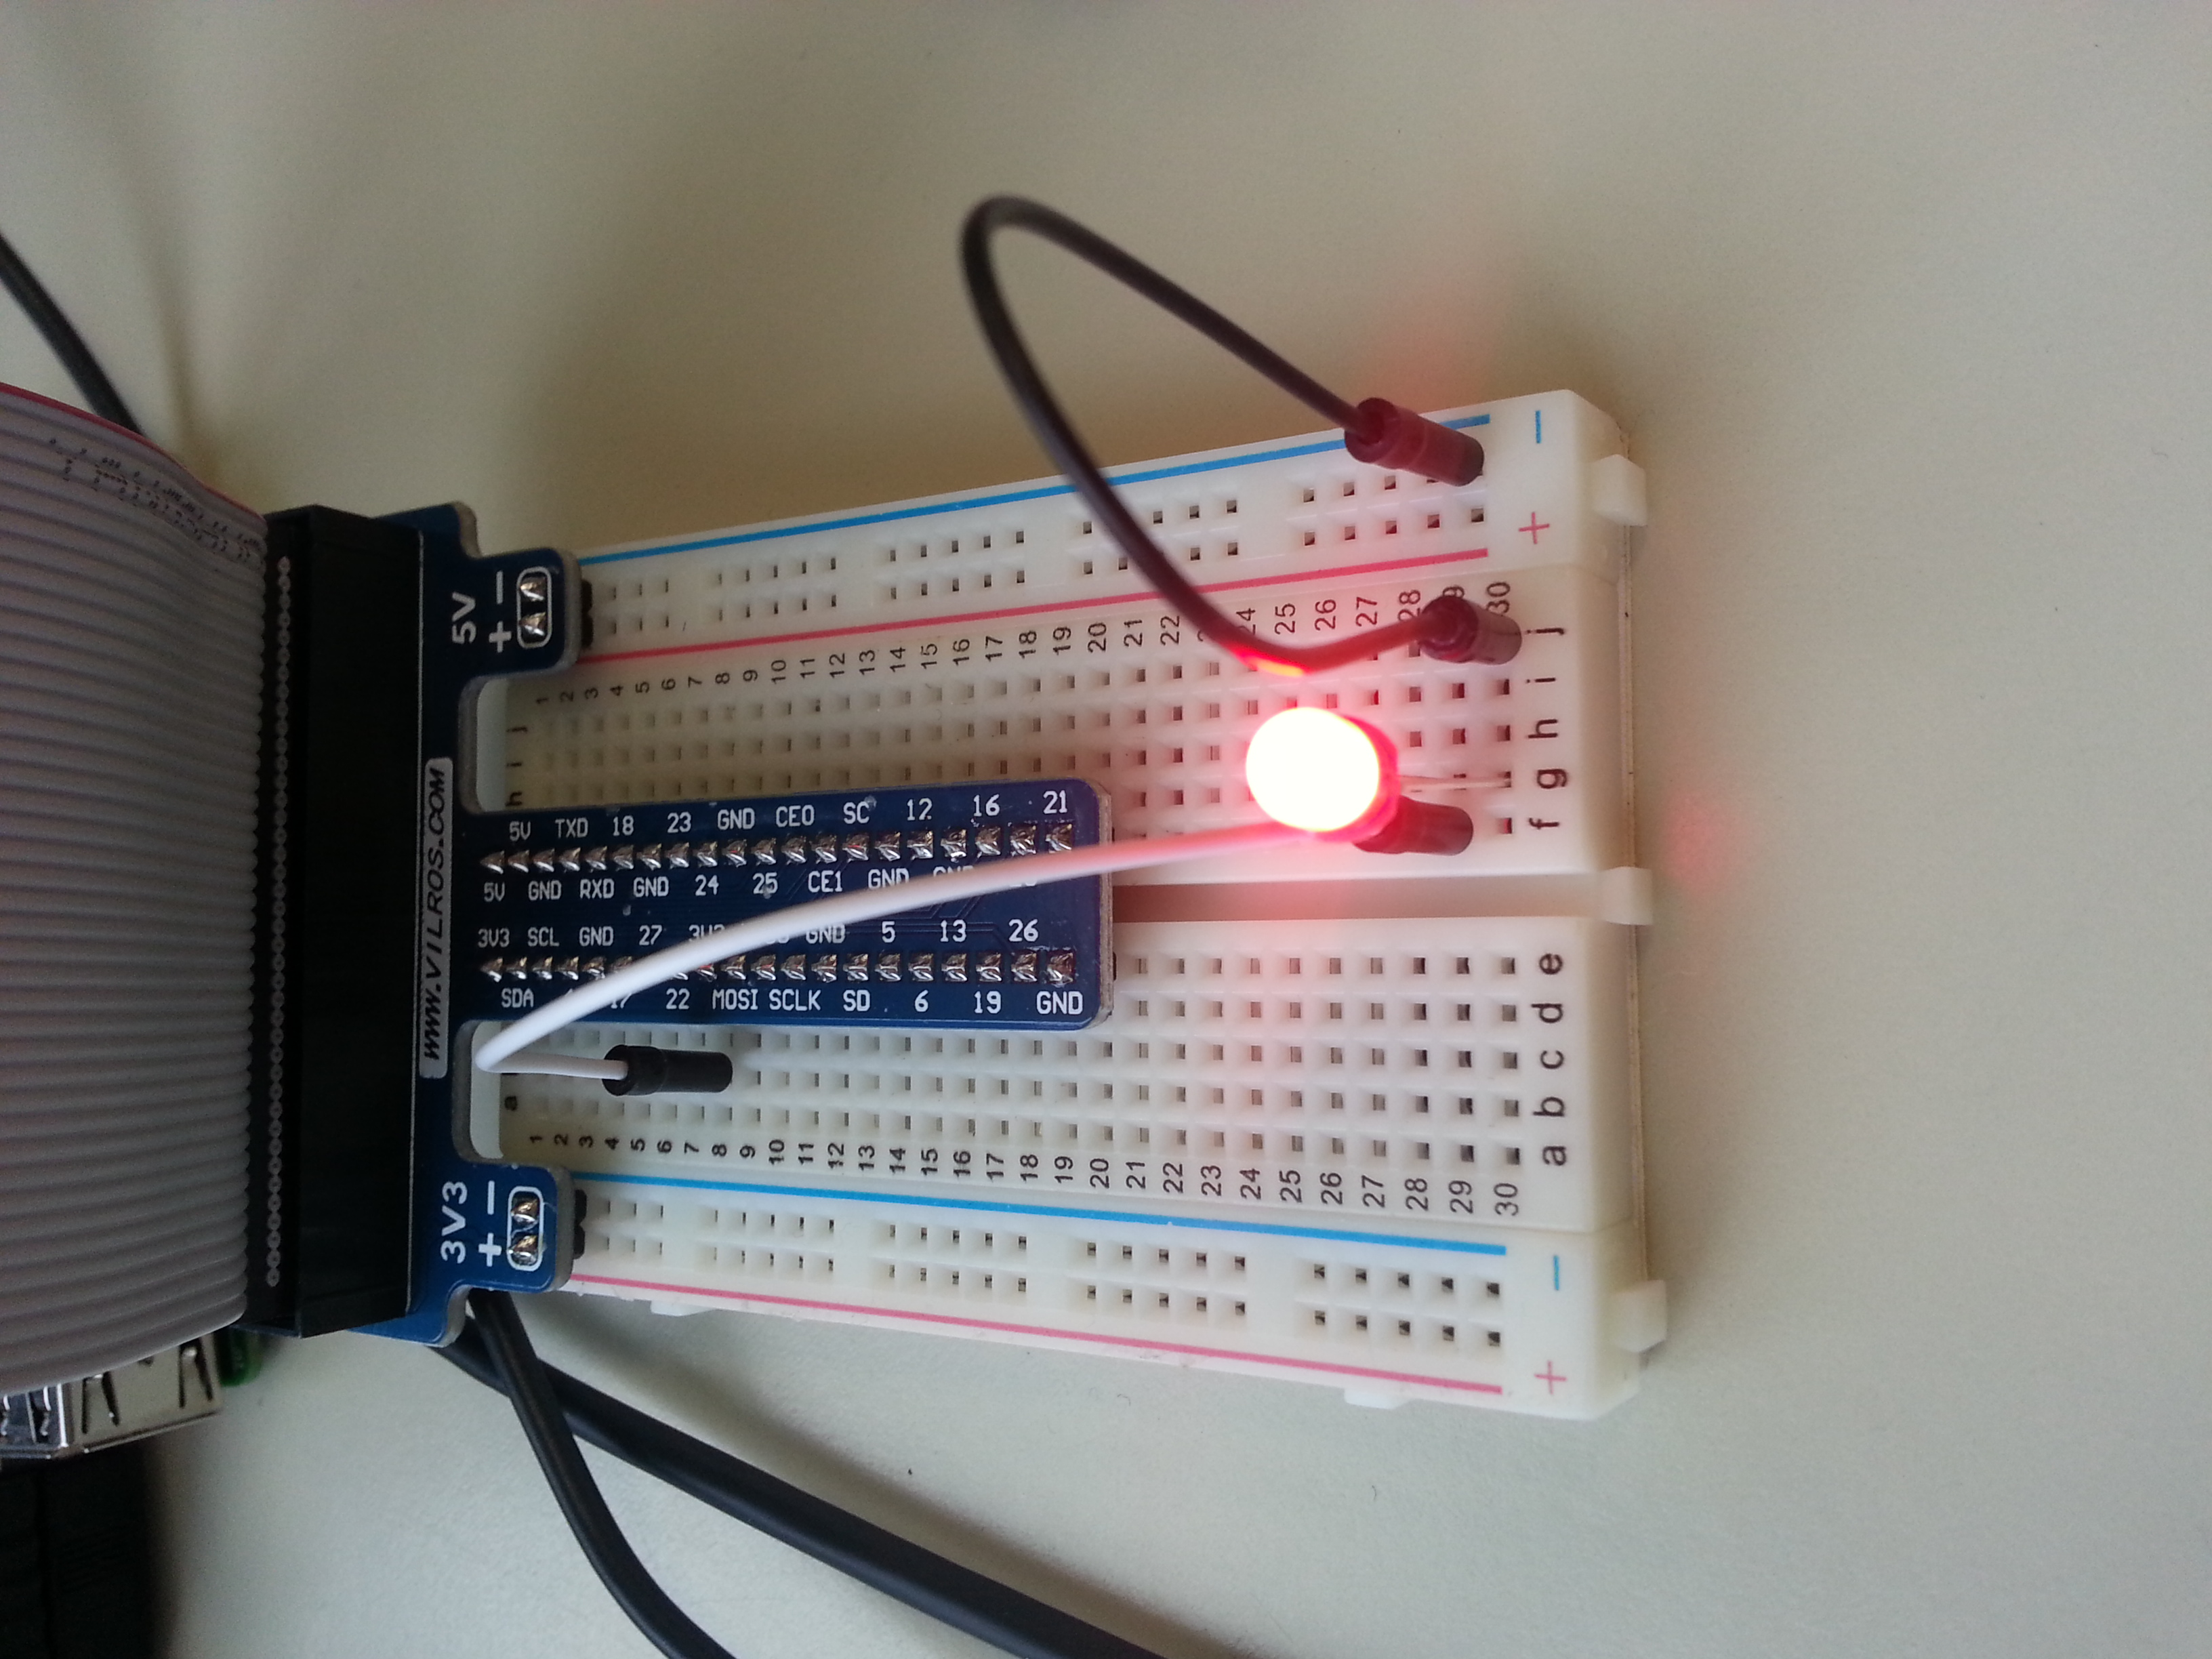
\includegraphics[width=\textwidth]{Test_unitaire/Rpi/img3.jpg}
  \caption{Allumage d'une LED par Raspberry Pi}
  \label{figure:led}
\end{figure}

\begin{figure}[!h]
  \centering
  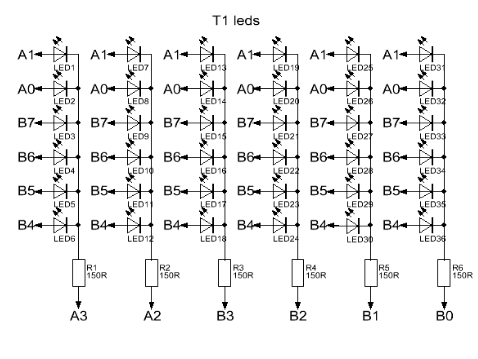
\includegraphics[width=0.8\textwidth]{Test_unitaire/Rpi/led.png}
  \caption{Méthode de connexion des leds dans le Montréal}  
  \label{figure:ledMontreal}
\end{figure}
\begin{figure}[!h]
  \centering
  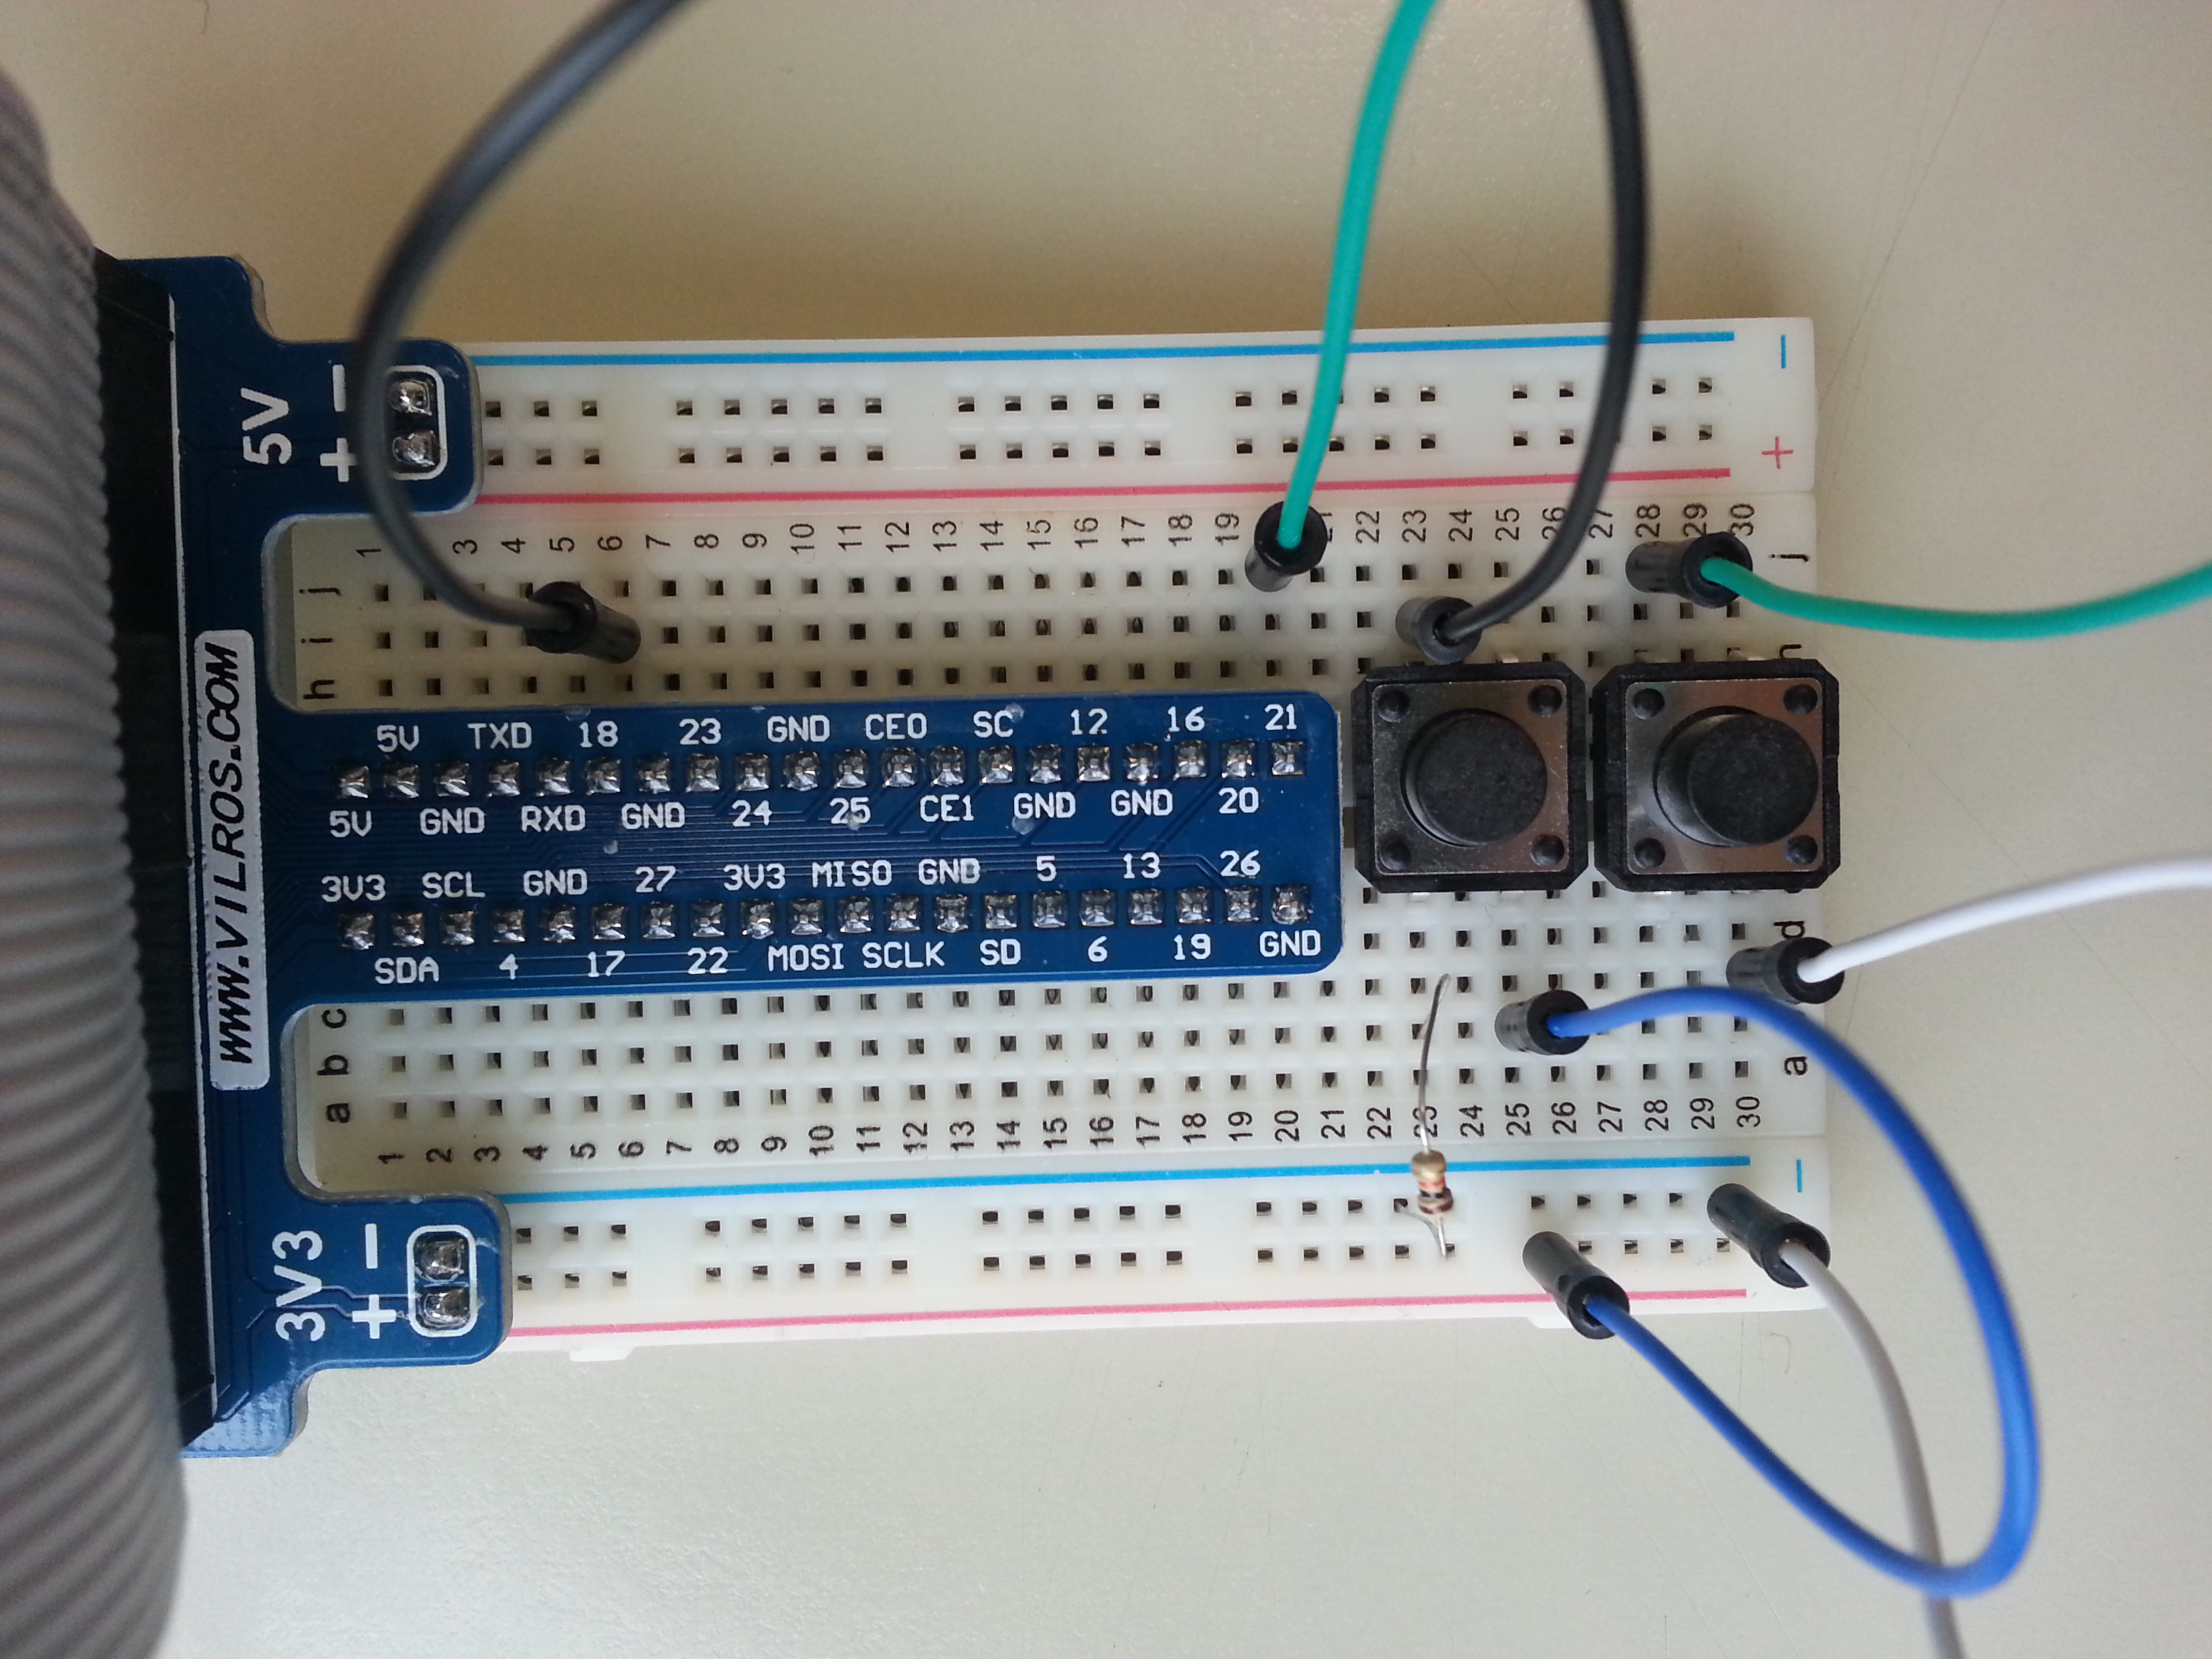
\includegraphics[width=\textwidth]{Test_unitaire/Rpi/img4.jpg}  
  \caption{Système modélisant une LED}
  \label{figure:test}
\end{figure}

La sortie du Montréal 3v2 est décrite à la figure \ref{figure:ledMontreal}. On constate que le pic qui permet l'affichage à 12 sortie qui lui permet de gérer 24 LED. Pour connaître quelle LED est allumé, il faut savoir laquelle des entré A1,A0,B7,B6,B5,B4 à un front montant et laquelle des entrées B0,B1,B2,B3,A3,A2 à un front descendant.

Pour modéliser une LED en entré du Raspberry Pi, nous avons positionné 2 boutons poussoirs (voir figure \ref{figure:test}). Le premier permets de réaliser le front montant et le second le front descendant. Ainsi en positionnant ces boutons au bon endroit par rapport au port GPIO du raspberry il est possible de connaître quelle LED on a simuler.

Nous avons réaliser un script python qui lié les entrées du raspberry avec les sortie du pic. Puis nous avons tester en simulant une LED comme décrit précédemment.

On peut constater que l'expérience est un succès car le raspberry pi nous renvoie bien le numéro de la LED que nous voulions tester.




%%%%%%%%%%%%%%%%%%%%%%%%%%%%%%%%%%%%%%%%%%%%%%%%%%%

\section{PIC}
\label{sec:pic}

Dans le schéma du Montréal 3v2 nous avons pu constater qu'il y avait 3 PIC programmés. Nous avons commandé les PIC programmés au près de l'entreprise F1LVT \cite{montreal}.


\begin{figure}[!h]
  \centering
  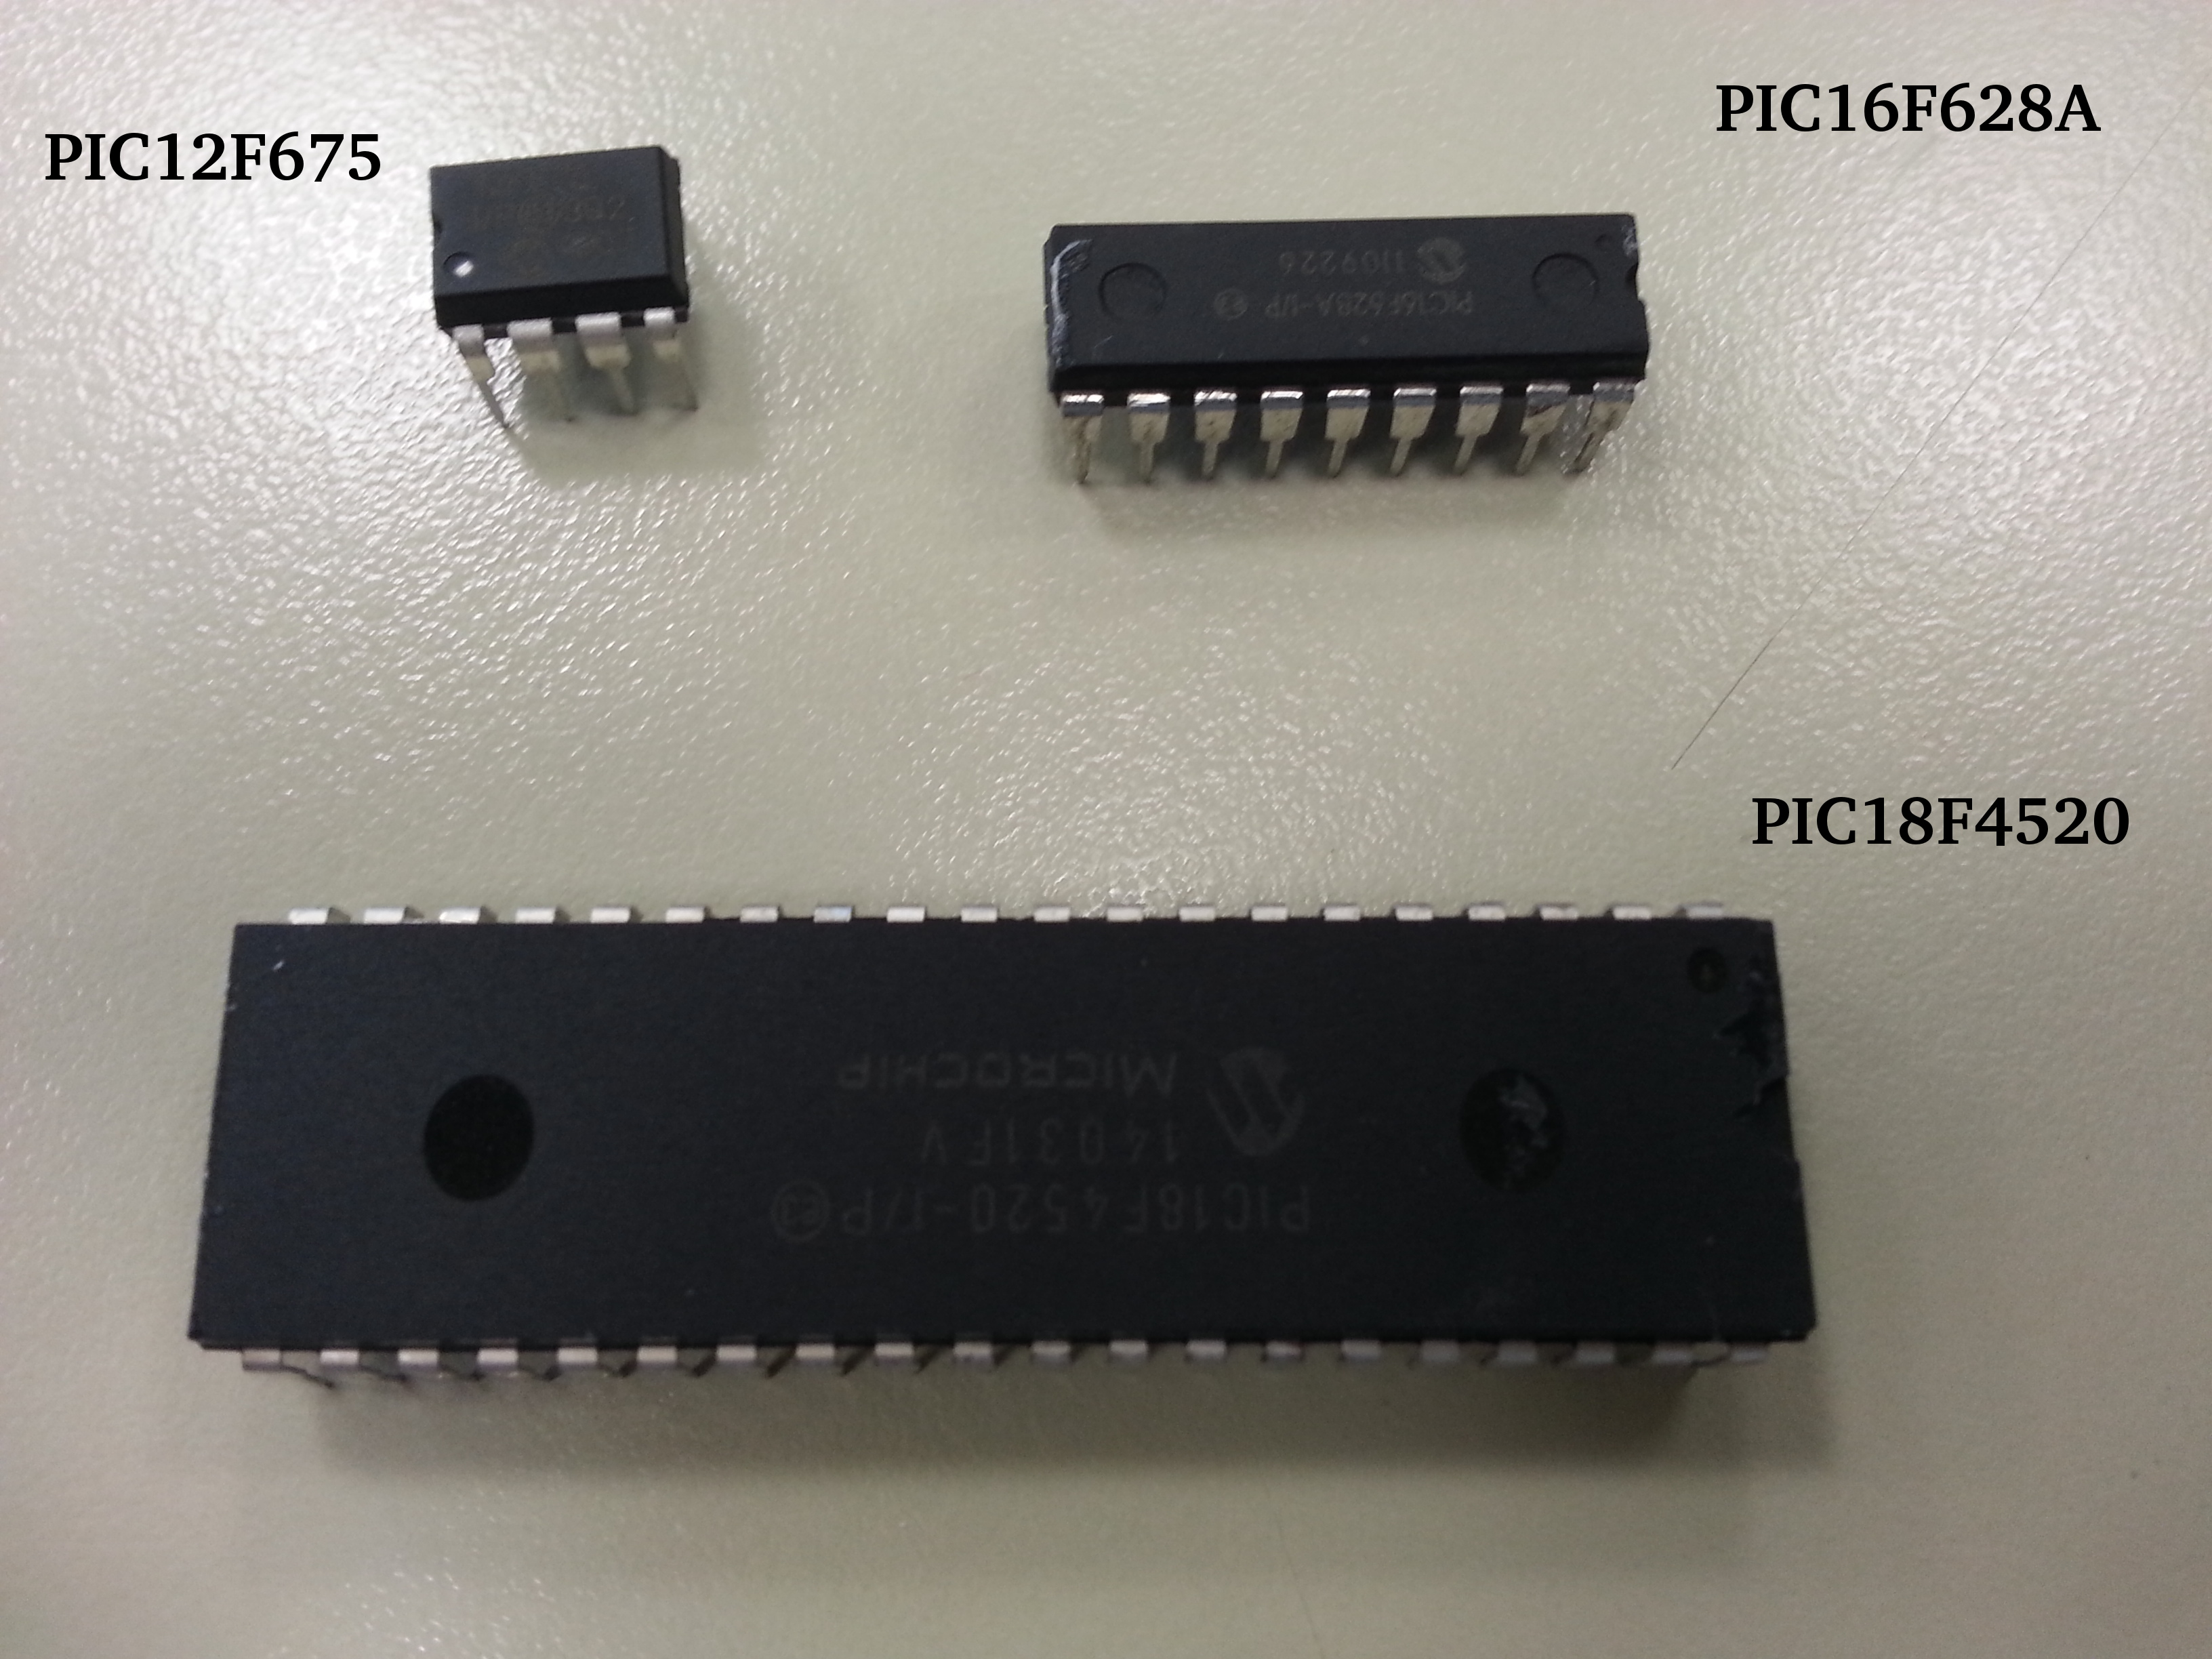
\includegraphics[width=\textwidth]{Test_unitaire/Pic/pic}
  \caption{3 PIC programmés}
  \label{fig:pic}
\end{figure}

Nous avons ensuite imaginé et réalisé des tests unitaires sur chacun des PIC pour vérifier qu'ils ont bien été programmés et qu'aucune erreur n'est apparu sur ce système de décision critique pour le système.

\subsection{PIC16F628A}
\label{sec:picled}

Ce PIC sert à réaliser l'affichage sur les LED. Pour tester ce PIC, nous avons réaliser le montage de la figure \ref{fig:picled}. On peut voir à la figure \ref{fig:schemapic} le schéma de montage du PIC sur le Montréal 3v2.

\begin{figure}[!h]
  \centering
  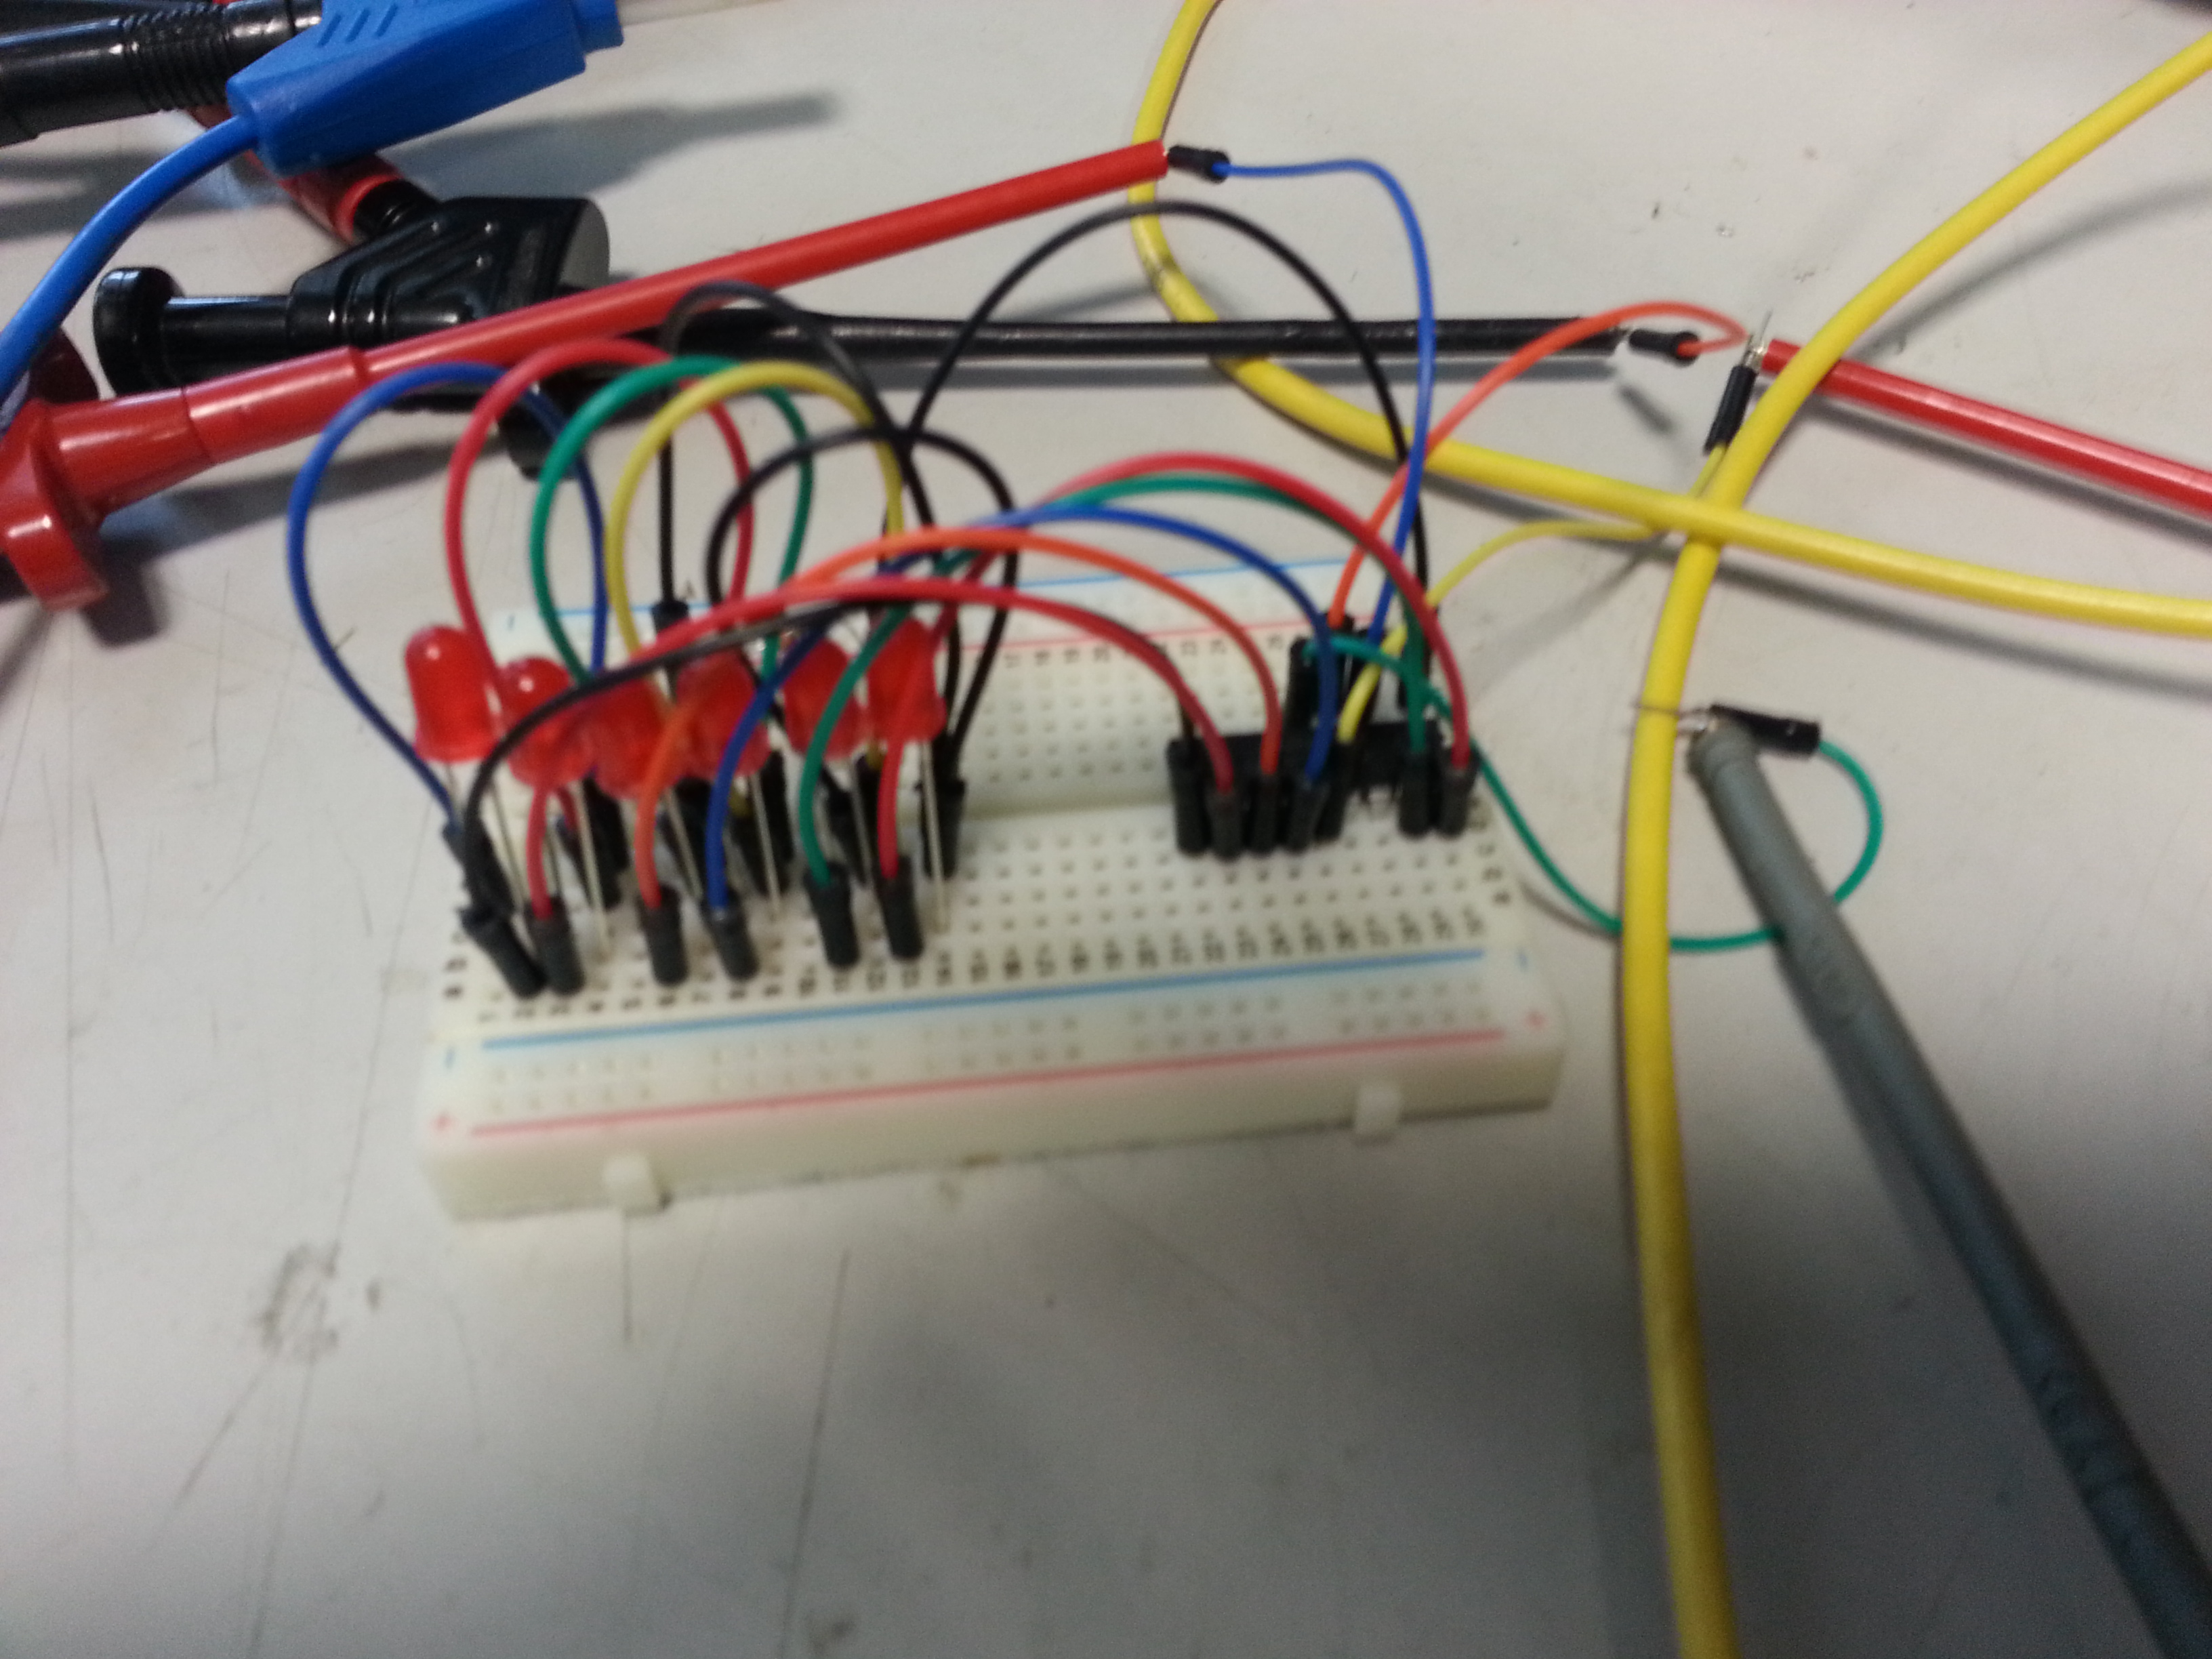
\includegraphics[width=\textwidth]{Test_unitaire/Pic/picled}
  \caption{Schéma electrique du test unitaire}
  \label{fig:picled}
\end{figure}


Pour tester ce composant, nous avons donc choisi de monter une partie des LED situés en sorti, de configurer le \og clock\fg{} sur un signal carré de fréquence 1 MHz, et de faire varier la fréquence de l'entrée \og data\fg{}.

Malheureusement nous n'avons pas pu observer de LED s'allumer pendant notre expérience.

\begin{figure}[!h]
  \centering
  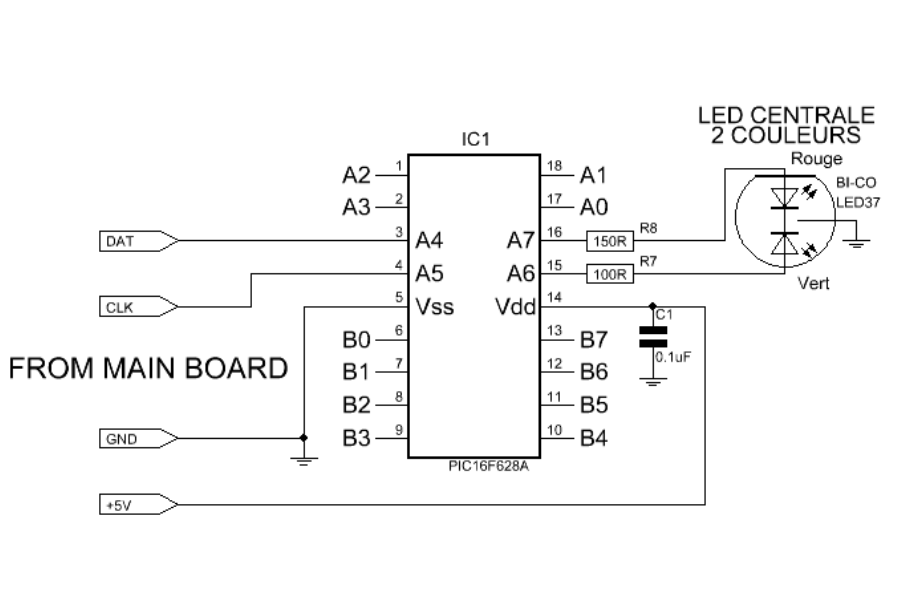
\includegraphics[width=\textwidth]{Test_unitaire/Pic/schemapic}
  \caption{Schéma de montage du pic sur le Montréal 3v2}
  \label{fig:schemapic}
\end{figure}

\subsection{PIC12F675}
\label{sec:picclock}

\subsection{PIC18F4520}
\label{sec:piccontrol}



%%% Local Variables: 
%%% mode: latex
%%% TeX-master: "../rapport"
%%% End: 


\chapter{Test d'intégration}

Nous n'avons malheureusement pas pu faire la totalité des tests d'intégrations puisque à la fin de notre projet nous n'avions pas la totalité des composants pour monter notre radio-goniomètre. Néanmoins nous avons pu tester l'intégration du radio-goniomètre au \rpi en plaçant des leds sur les ports GPIO \footnote{Les ports GPIO sont des entrées/sorties analogiques présentes sur la carte du raspberry}, ainsi que l'intégration de l'application mobile au serveur central.


\section{Raspberry Pi}
La documentation technique liée a notre Raspberry Pi est située en annexe à la page \pageref{annexe:rpi}
~\\

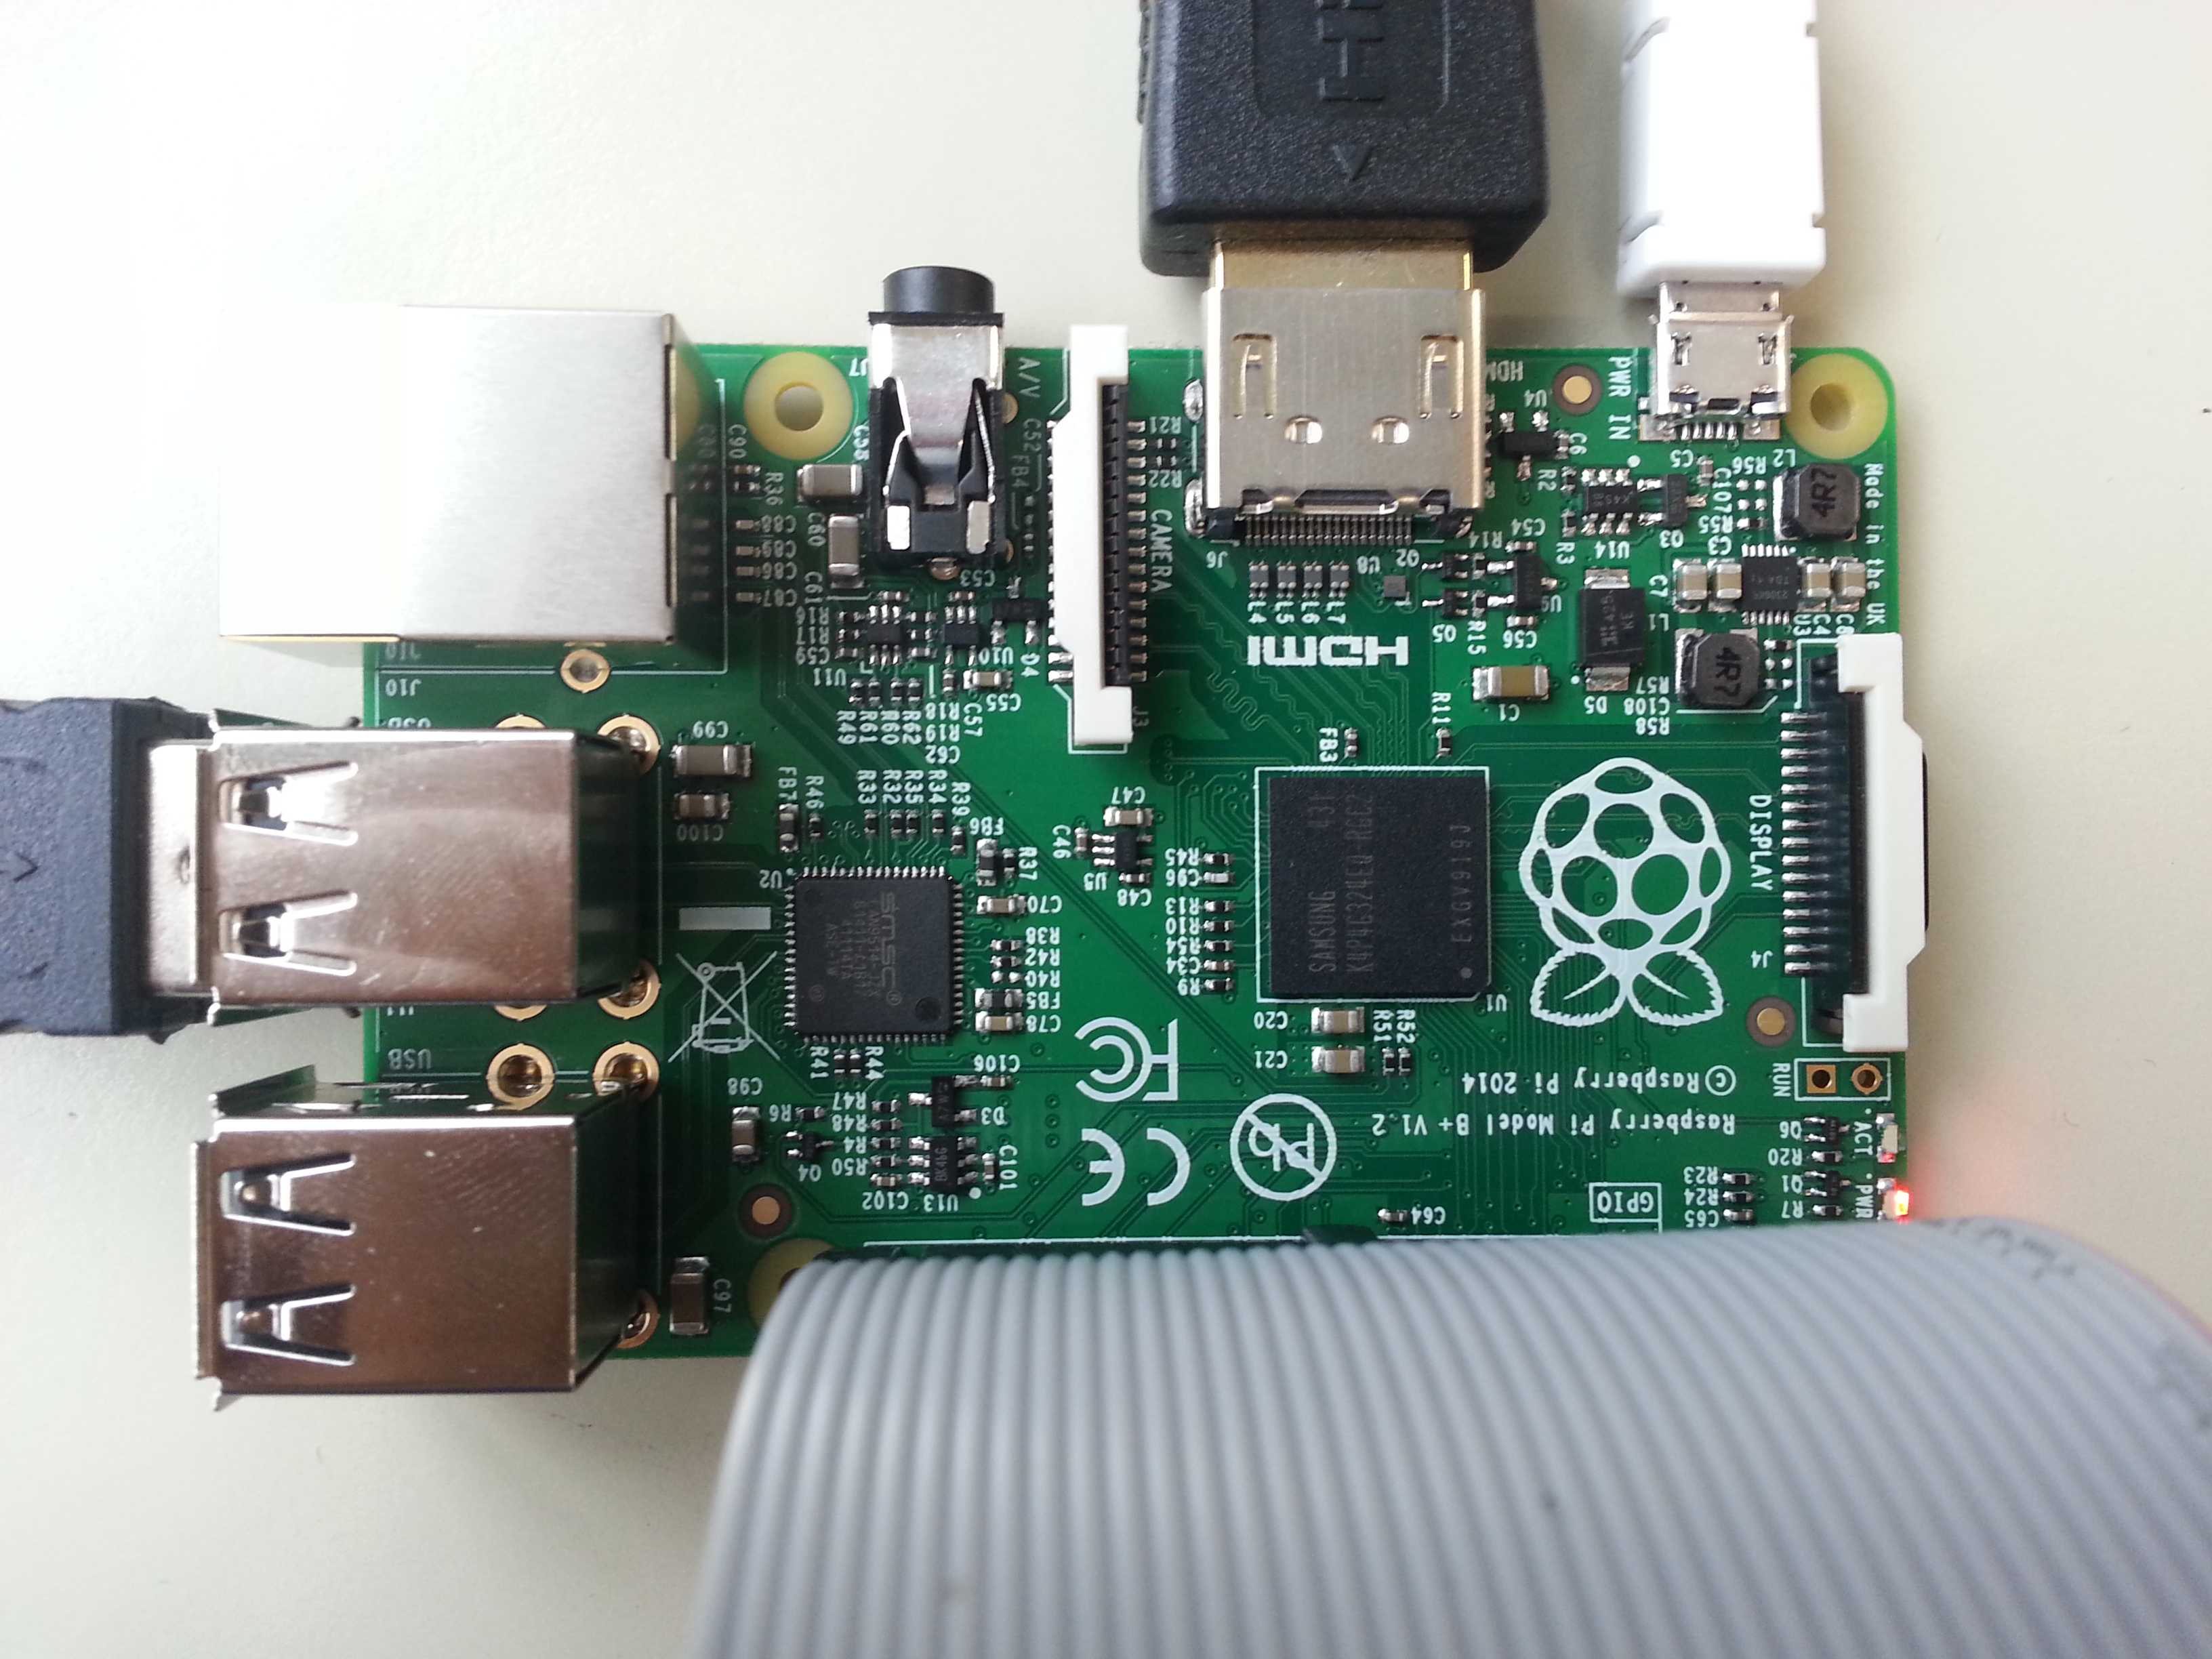
\includegraphics[width=\textwidth]{Test_unitaire/Rpi/img5.jpg}
\captionof{figure}{Notre Raspberry Pi B+}

~\\
\parindent=15pt

Pour s'assurer que notre Raspberry Pi répond aux spécifications fonctionnelles et qu'il fonctionne correctement en toutes circonstances pour notre projet, nous y avons réalisé des tests intégrations.

Après avoir enfin installé le système d'exploitation Raspbian\footnote{La documentation lié à Raspbian est situé en annexe à la page \pageref{annexe:raspbian}} sur notre Raspberry Pi B+, nous avons tenté de tester les ports GPIO. Pour cela, dans un premier temps, nous avons allumé des LED grâce à un script python à travers différents ports GPIO. Sur la figure \ref{figure:led}, on peut observer que nous avons allumé une LED grâce au port 22.
~\\

Dans notre projet le Raspberry Pi sera placé entre le radio-goniomètre à effet Doppler et l'utilisateur. Il aura deux taches, corréler les données entre tous les dispositifs pour obtenir la position du drone et afficher le résultat à l'utilisateur. Pour cela il doit récupérer la direction qui est donnée par le Montréal 3v2. Cette position est donnée à travers des LED (voir figure \ref{figure:ledMontreal}). Nous allons donc placer le Raspberry Pi au niveau des LED pour obtenir les informations délivrées par le Montréal 3v2. % TODO : A FINIR

\begin{figure}[!h]
  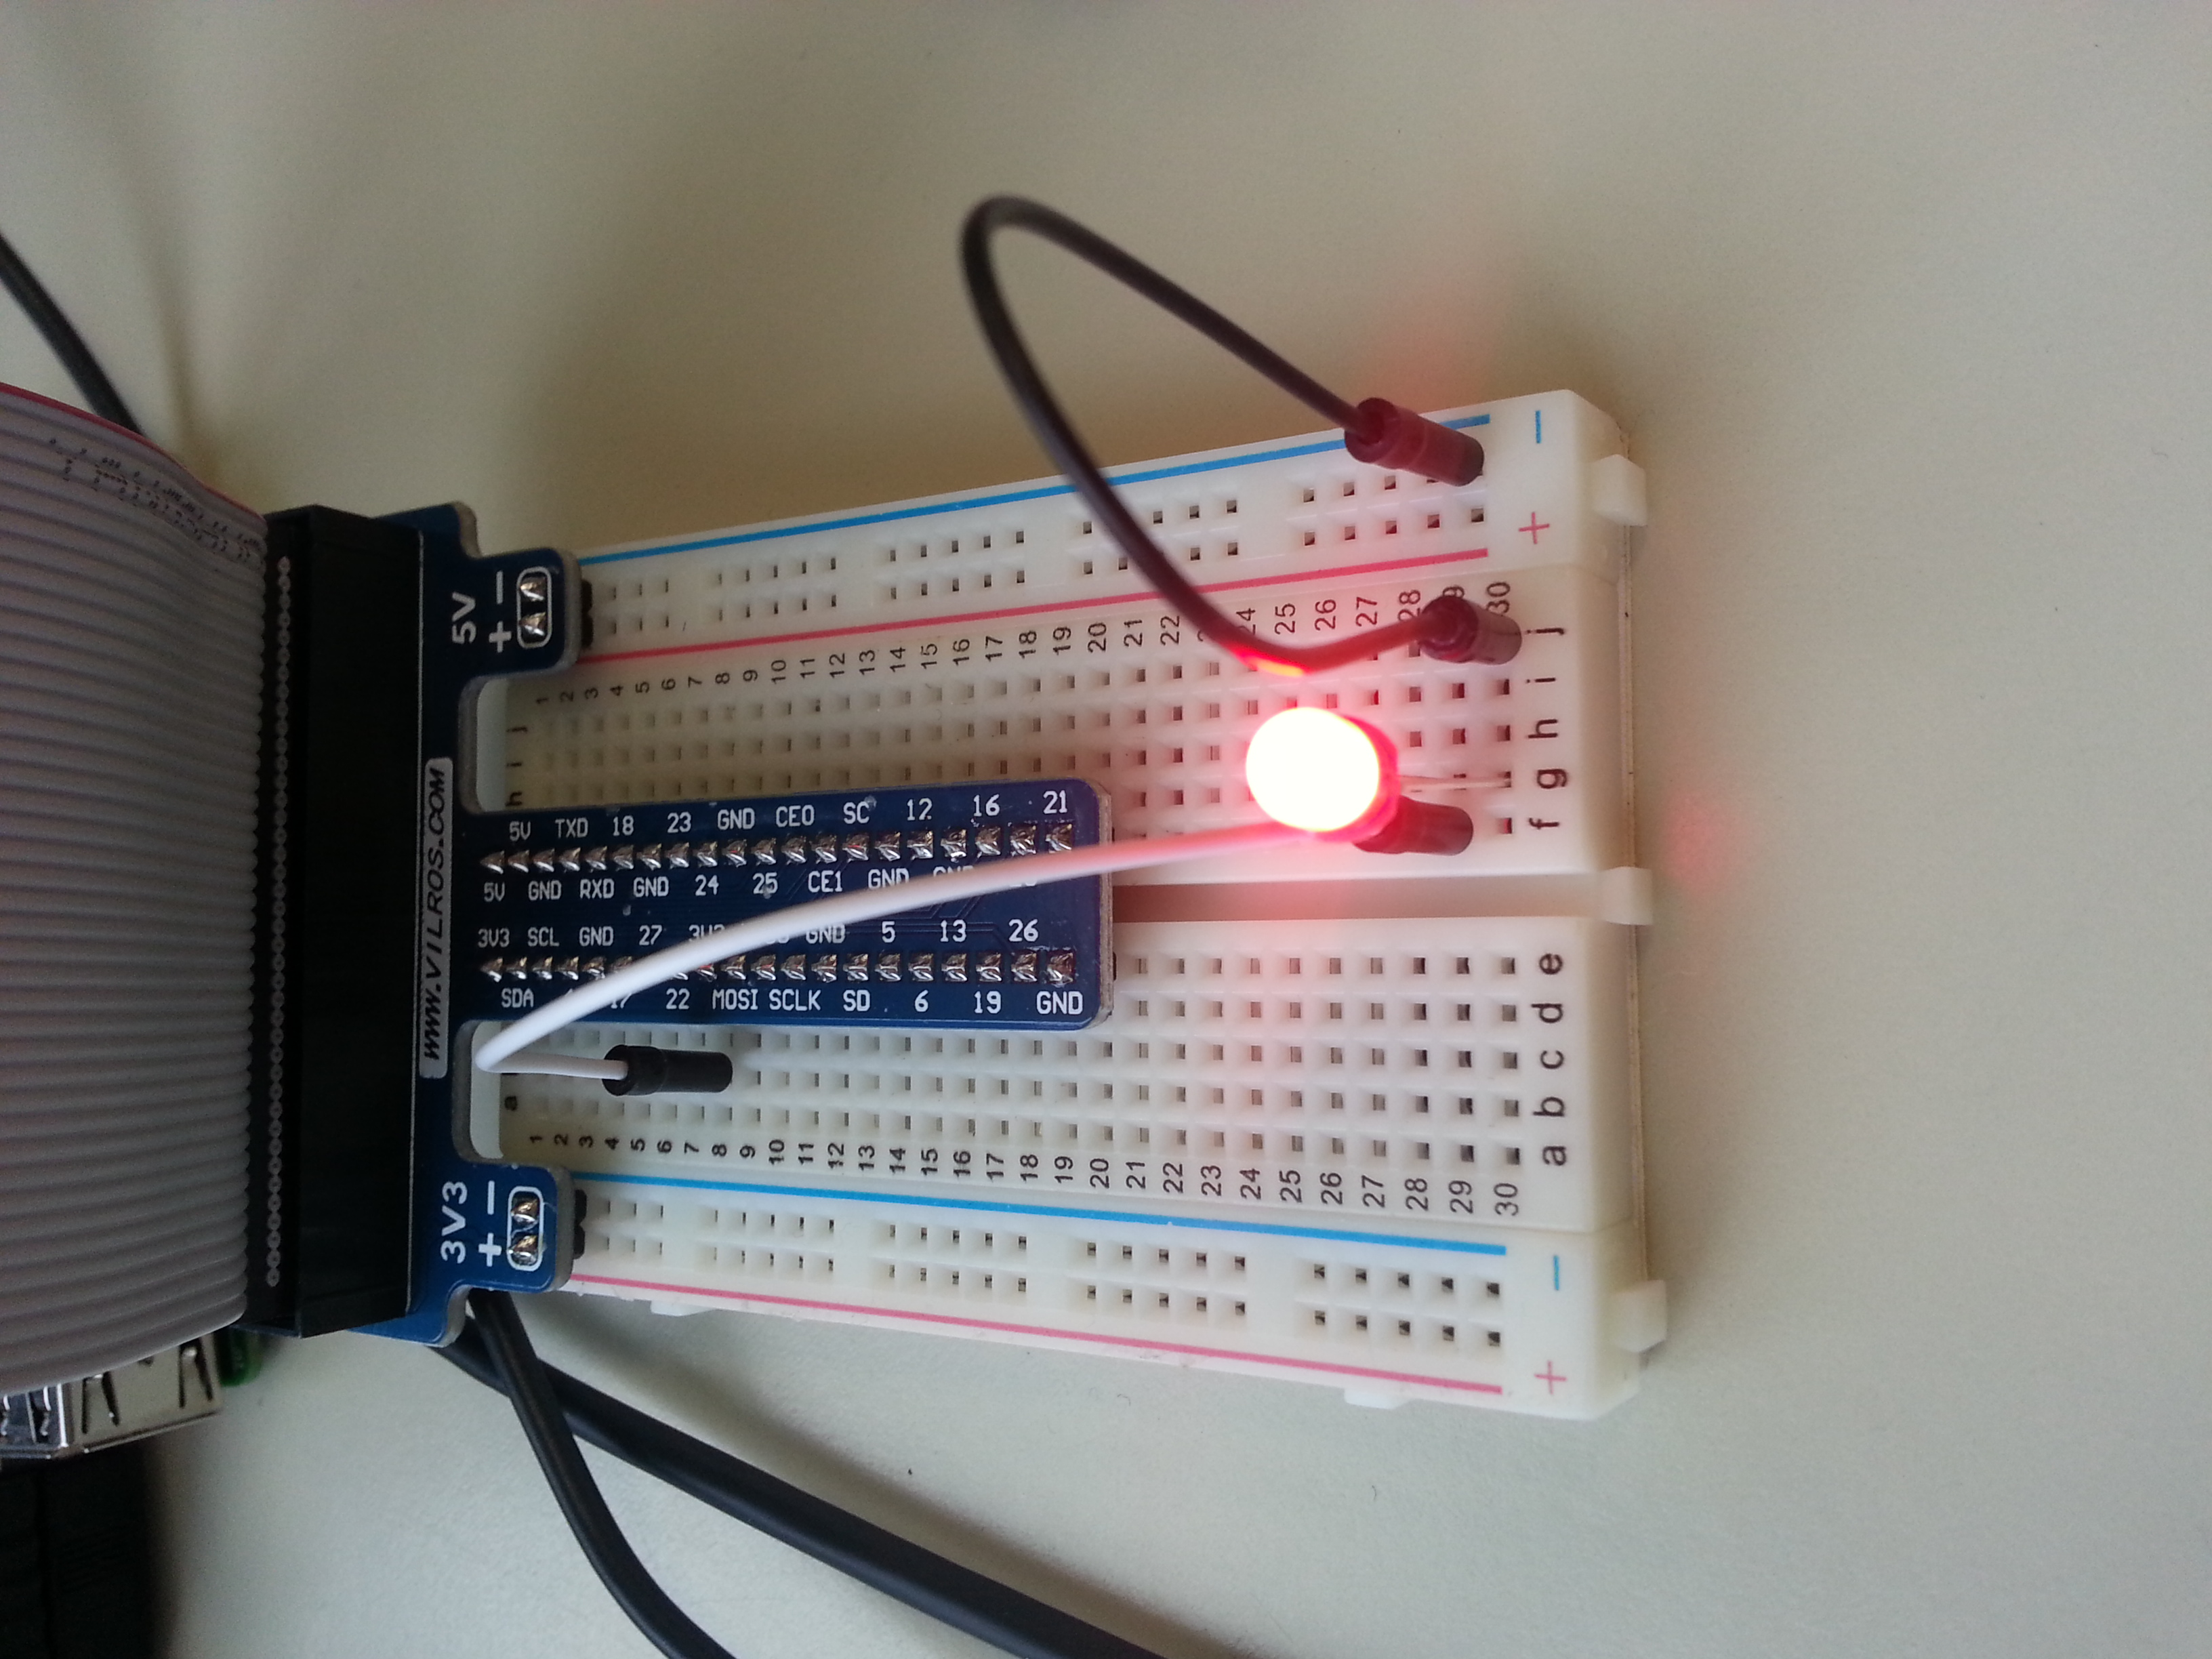
\includegraphics[width=\textwidth]{Test_unitaire/Rpi/img3.jpg}
  \caption{Allumage d'une LED par Raspberry Pi}
  \label{figure:led}
\end{figure}

\begin{figure}[!h]
  \centering
  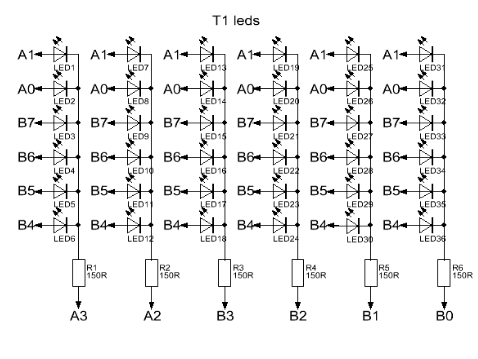
\includegraphics[width=0.8\textwidth]{Test_unitaire/Rpi/led.png}
  \caption{Méthode de connexion des leds dans le Montréal}  
  \label{figure:ledMontreal}
\end{figure}
\begin{figure}[!h]
  \centering
  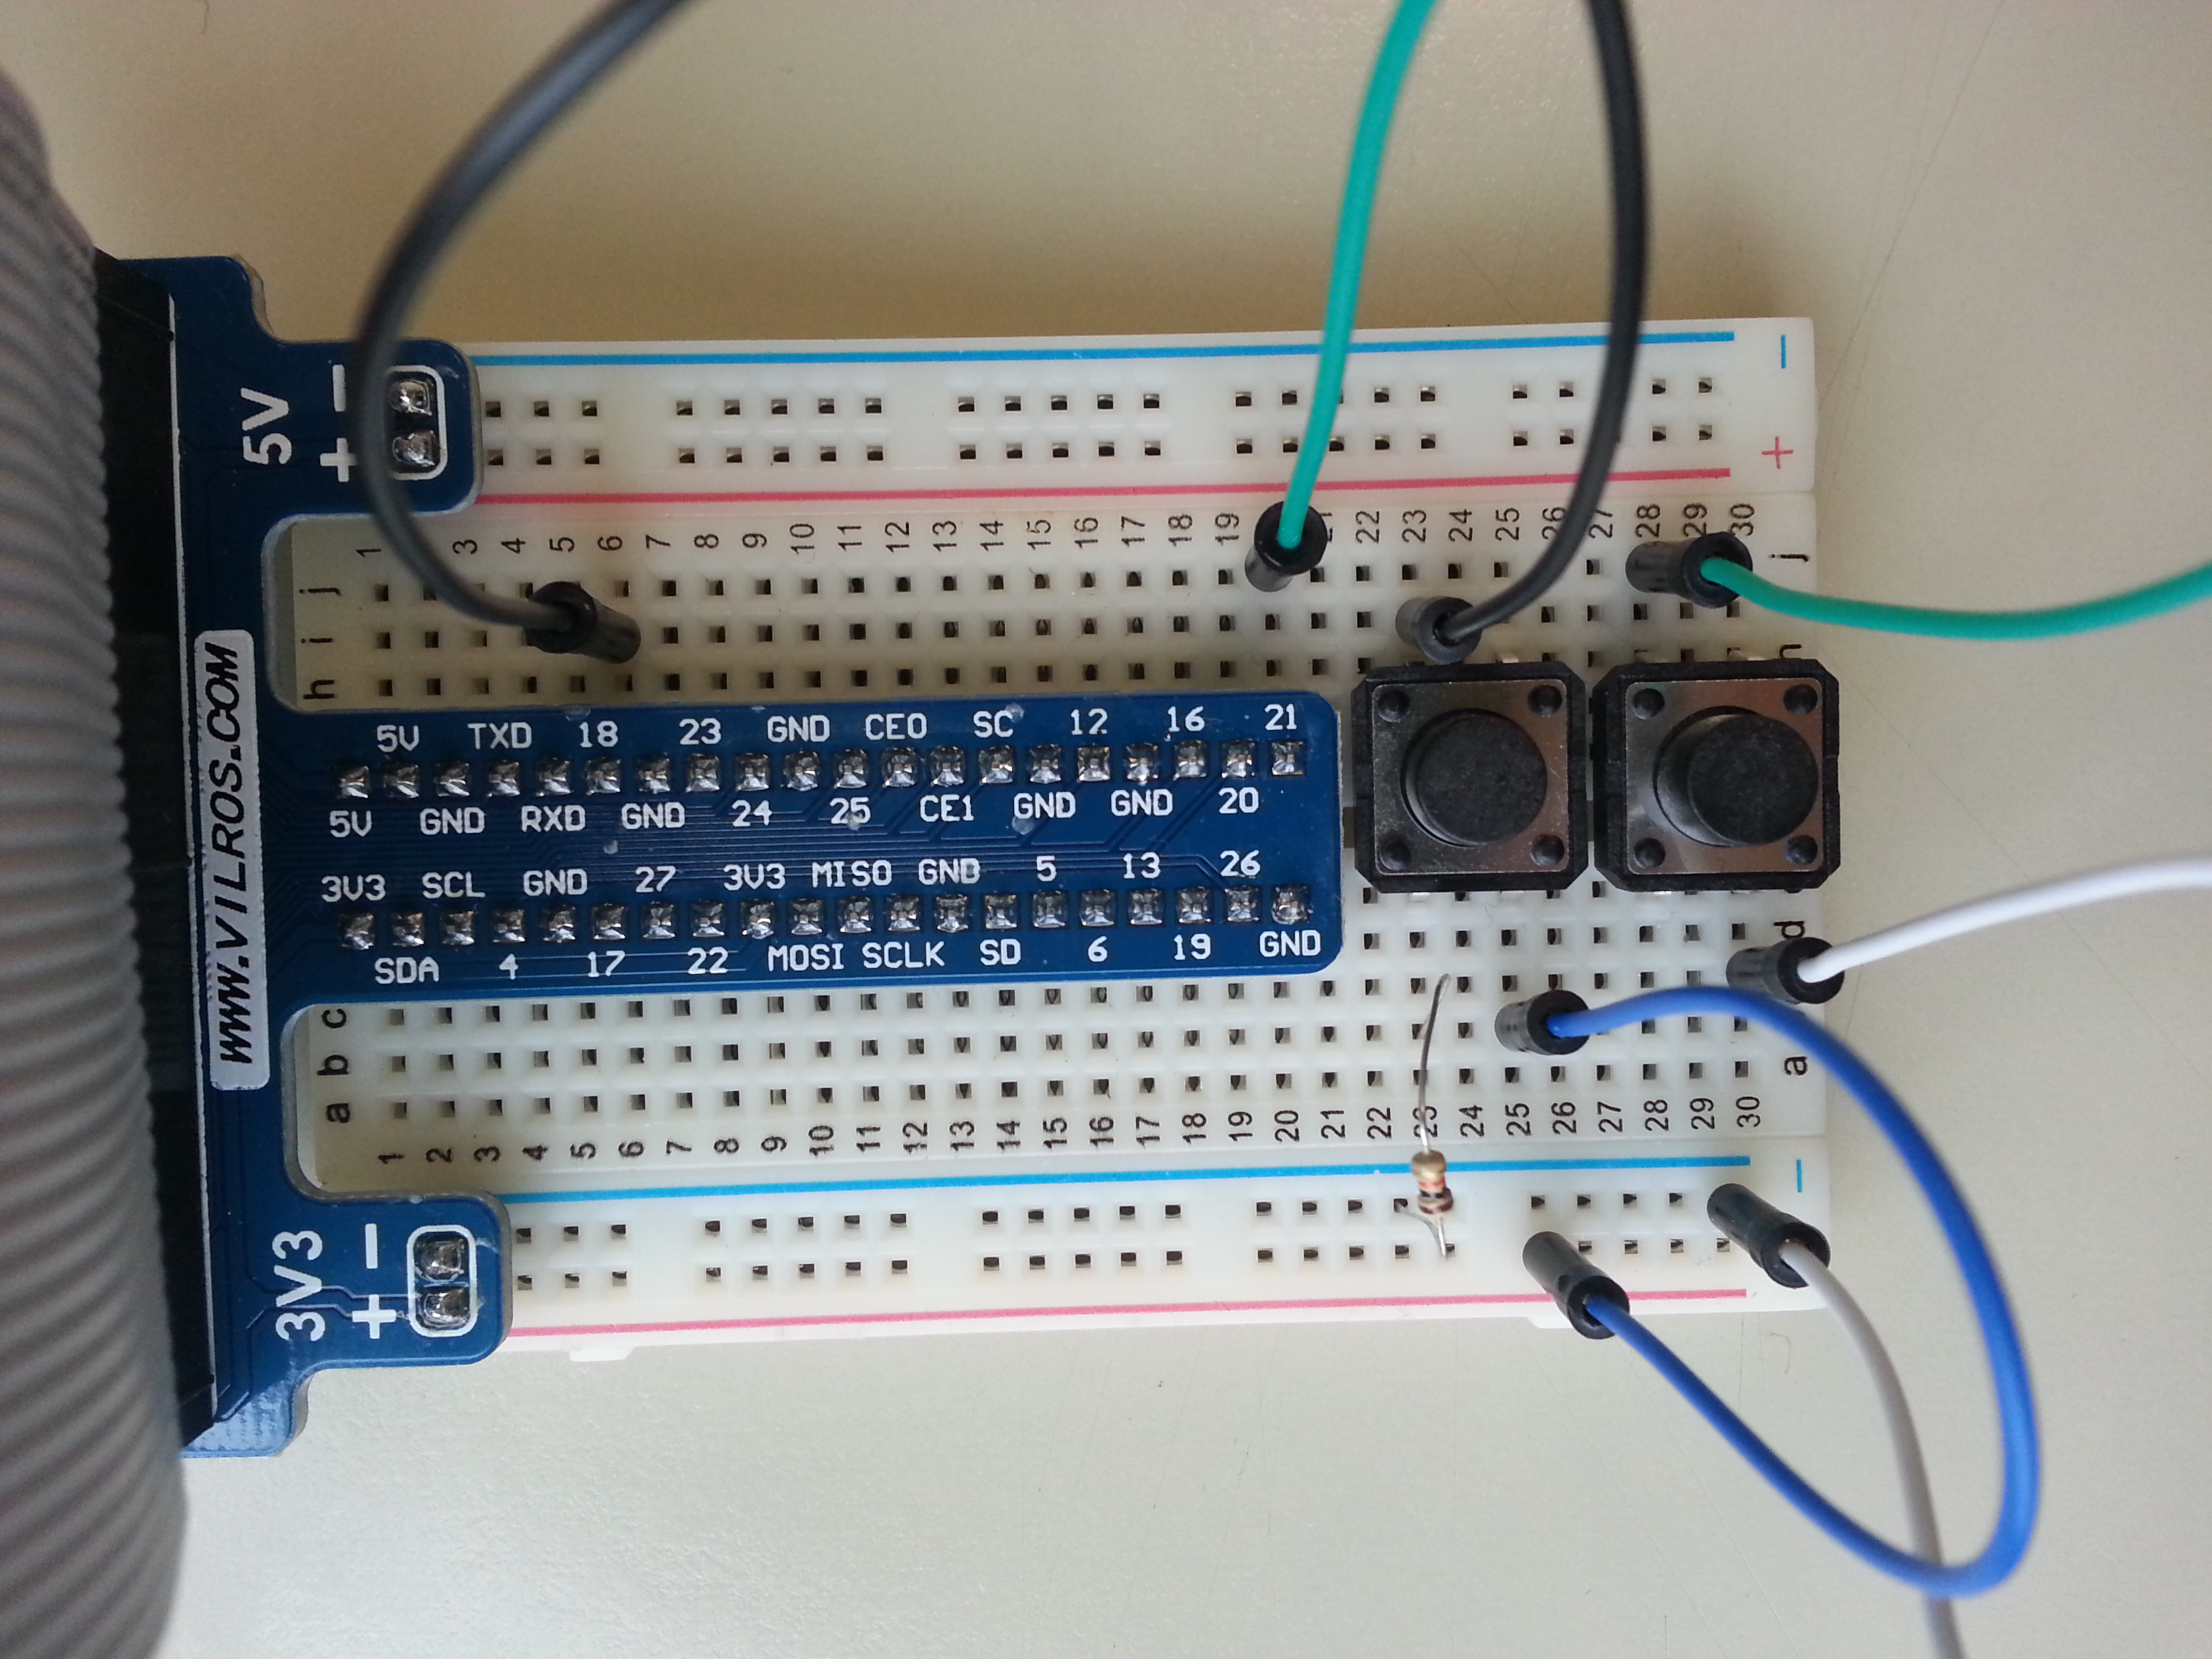
\includegraphics[width=\textwidth]{Test_unitaire/Rpi/img4.jpg}  
  \caption{Système modélisant une LED}
  \label{figure:test}
\end{figure}

La sortie du Montréal 3v2 est décrite à la figure \ref{figure:ledMontreal}. On constate que le pic qui permet l'affichage a 12 sortie lui permettant de gérer au total 24 LEDs. Pour savoir quelle LED est allumée, il faut savoir laquelle des entrées A1,A0,B7,B6,B5,B4 voit un front montant en signal d'entrée et laquelle des entrées B0,B1,B2,B3,A3,A2 voit un front descendant.

Pour modéliser une LED en entrée du Raspberry Pi, nous avons positionné 2 boutons poussoirs (voir figure \ref{figure:test}). Le premier permet de simuler un front montant et le second un front descendant. Ainsi en positionnant ces boutons au bon endroit par rapport au ports GPIO du raspberry il est possible de connaître quelle LED on a simulé.

Nous avons réalisé un script python qui lie les entrées du raspberry avec les sorties du pic. Puis nous avons testé en simulant une LED comme décrit précédemment.

L'expérience est un succès car le raspberry pi nous renvoie bien le numéro de la LED que nous voulions tester sur la console linux ouverte en parallèle.


\section{Android}

Les premiers tests de l'application Android étaient de simples tentatives de connections avec transmission de messages simples pour vérifier le bon fonctionnement des socket Web. 
Une fois l'application terminée une série de tests plus complets ont été effectués pour simuler le comportement global de l'application en conditions réelles.
~\\
Le premier test d'intégration réalisé simule une succession de quatres instances de communication entre le client Android et le serveur. L'objectif est de simuler la transition d'un état "Rien à Signaler" vers un état "Drone détecté", et de vérifier l'exactitude des informations transmises. Pour visualiser le comportement du téléphone nous avons utilisé l'outil "logcat" du logiciel de programmation Android Studio qui permet de visualiser en temps réel les registres du téléphone. 

\begin{figure}[!h]
  \centering
  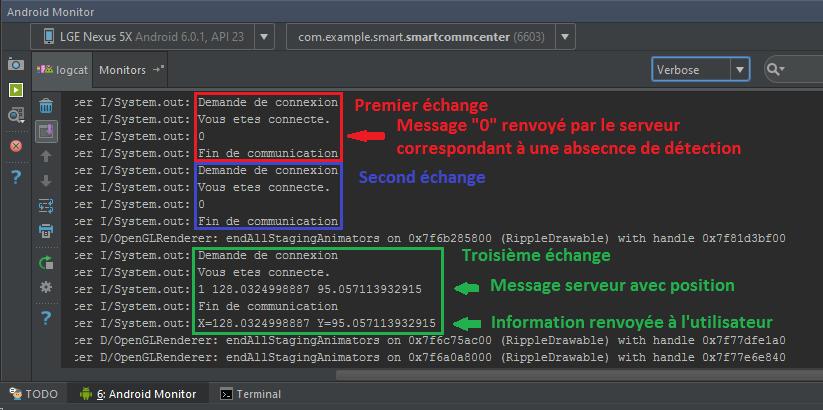
\includegraphics[width=\textwidth]{logcat}  
  \caption{Premier test : communication}
\end{figure}

Sur cette image on peut visualiser les trois premiers échanges. Les deux premières requêtes ne donne lieu à aucun changement sur l'application car aucun drone simulé n'a été détecté.
Le troisième échange résulte de l'entrée d'un drone dans la zone simulée. On d'abord peux visualiser le message brut reçu par l'application puis dans un second temps la chaine de caractères formatée par l'application avant qu'elle soit affichée par l'interface.
~\\
Le second test d'intégration lié à l'application avait pour but de vérifier le bon affichage des erreurs de connexion sur l'application Android pour éviter toute ambiguïté. 

\begin{figure}[!h]
  \centering
  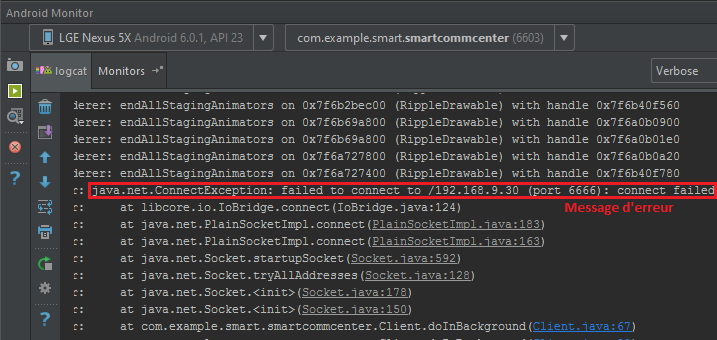
\includegraphics[width=\textwidth]{log_error}  
  \caption{Second test : erreurs}
\end{figure}

\newpage %% a virer si ça gène

\begin{wrapfigure}{r}{0.5\textwidth}

  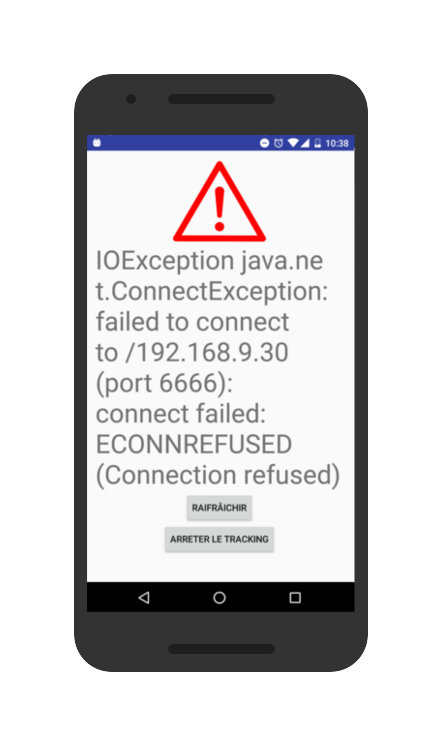
\includegraphics[width=0.25\textwidth]{error_co}
  \caption{Message d'erreur sur l'application}
\end{wrapfigure}

En cas d'erreur le message est bien visible dans les logs et L'application ne s'est pas bloquée. Celle-ci sera donc capable de bien différencier une absence de détection d'une erreur de connections tout en restant prête à renvoyer une requête au serveur. De plus, le message d'erreur est bien affiché dans son intégralité sur l'interface de l'application. elle est ici réglée en mode "Debug" pour afficher un maximum d'informations.



%%% Local Variables: 
%%% mode: latex
%%% TeX-master: "../rapport"
%%% End: 
\part{Réalisation}



\chapter{Radiogoniometre}

 
\section{Module Montréal}

Le module Montréal comprends deux cartes électroniques : la carte principale qui est chargée de toutes les tâches relatives au traitement du signal reçu par les antennes et la carte destinée à l'affichage de la direction.

Les supports des cartes sont en résine époxy sur laquelle ont été apposée des pistes en cuivre en configuration mono-couche (les pistes ne sont présentes que sur une face de la plaque). Un étamage par dépôt chimique des piste a été réalisé pour les protéger de l'oxydation. L'ensemble de ces opération ont été effectuées à l'école avec l'aide de Mr. Gallou.
 
Le PIC18F4520 chargé de la majorité des traitements et le PIC12F675 ont été soudés sur la carte principale. Le PIC16F628A, chargé de l'affichage des LEDs a été soudé sur la carte d'affichage de direction. Le montage choisi pour ce dernier PIC permet de le désolidariser de la plaque afin d'effectuer les tests d'allumage des LEDs de direction.

L'ensemble des composants que nous avions a disposition (LEDs, condensateurs et résistances) ont été ensuite soudés sur les deux plaques. 

Par rapport au montage d'origine nous n'utiliseront pas le RS232. Toutefois, lors de la rédaction de ce rapport, il manque deux filtres sur la carte principale qui nous empêchent de valider son fonctionnement.


\section{Down converter}


\begin{wrapfigure}{r}{0.4\textwidth}
  
  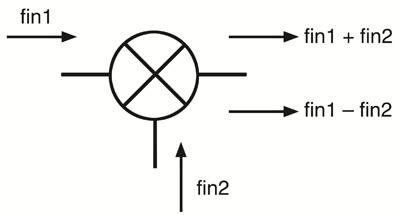
\includegraphics[width=0.4\textwidth]{mixer}
  \caption{schéma de fonctionnement d'un mixer}
\end{wrapfigure}


Le radiogoniomètre Montréal 3v2 fonctionne à une fréquence de 500Mhz. Sans modification il est impossible de l’utiliser entre 2.4Ghz et 2.5 GHz, bande de fréquence utilisée par les drones que nous souhaitons détecter. Nous avons donc cherché un moyen d’adapter ce radio-goniomètre aux fréquences souhaitées.

Une solution applicable à notre système est l'utilisation d'un down-converter. Ce composant reçoit deux entrées, le signal dont on veut changer la fréquence(RF) et un signal de fréquence fixe Df(LO). Le down-converter diminue la fréquence du premier signal de celle du second. La sortie(IF) correspond au signal modifié. Son principe de fonctionnement est illustré à la figure \ref{fig:mix}.



\begin{figure}[h]
  \centering
  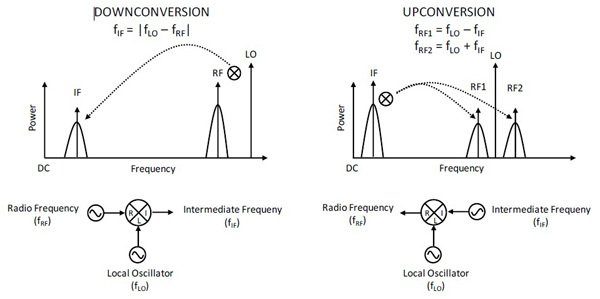
\includegraphics[width=\textwidth]{fonc_mixer}
  \caption{principe du fonctionnement d'un mixer}
  \label{fig:mix}
\end{figure}

On utilisera donc le down-converter pour abaisser la fréquence reçue par les antennes (2.4GHz) à la fréquence de travail du radio-goniomètre.

La fréquence du signal Df est donnée par un VCO (Voltage Controlled Oscillator ou oscillateur contrôlé en tension), le VCO reçoit en entrée une tension et donne en sortie une sinusoïdal de fréquence dépendante de la tension d’entrée. Le VCO étant très sensible, il est nécessaire de stabiliser la tension d’entrée et l’alimentation. On utilise donc un régulateur de tension qui amène une entrée stable. Le régulateur est un composant qui viendra limiter à une valeur seuil Vmax la tension qu'il reçoit en entrée si celle ci dépasse ce seuil. Dans le cas ou V < Vmax la sortie du régulateur sera égale à l'entrée.

Le VCO étant un composant actif et sensible aux variations dans sa tension d'alimentation, un second régulateur a été utilisé pour alimenter le VCO, toujours dans le but d’obtenir une fréquence stable ne variant pas pendant le processus. Il est en effet indispensable que cette fréquence reste fixe pour que l’effet doppler soit toujours visible et exploitable. Des fluctuations incontrôlées de la tension d'alimentation ou de la fréquence pourraient perturber la localisation.

Pour améliorer la mesure, il est utile de filtrer au maximum toutes les fréquences pouvant perturber la mesure et les différents bruits électromagnétiques. Ces phénomènes ont été atténués en positionnant en entrée du down-converter un filtre passe-bande qui permet de conserver uniquement la portion du spectre qui nous intéresse soit la bande située entre 2.4Ghz et 2.5Ghz.


\begin{figure}[h]
  \centering
  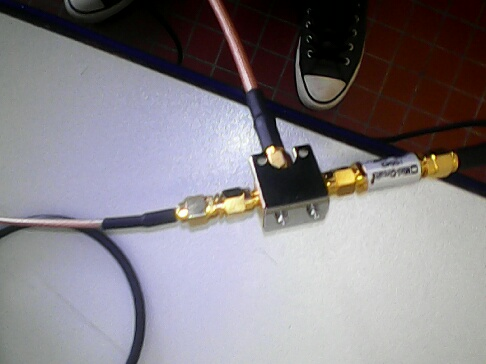
\includegraphics[width=0.5\textwidth]{down_converter}
  \caption{le down-converter et le filtre passe bande}
  \label{fig:down}
\end{figure}

A l’aide de ce montage on peut améliorer le signal en entrée pour qu'il puisse être traité correctement par le radio-goniomètre.

%%% Local Variables: 
%%% mode: latex
%%% TeX-master: "../rapport"
%%% End: 


\chapter{Interface Web}
\label{Logiciel}

Une foi le capteur terminé nous nous sommes penchés sur l'interface Homme/Machine. Dans une volonté de délivrer à l'utilisateur une interface agréable et lisible, nous avons décidé de proposer dans un premier temps une interface web.

\section{Analyse}
\label{sec:uml}

Dans un premier temps nous nous sommes penché sur une  phase d'analyse.

Dans la phase d’analyse, on cherche d’abord à bien comprendre et à décrire de façon précise les besoins des utilisateurs ou des clients concernant cette interface. Que souhaitent-ils faire avec le logiciel ? Quelles fonctionnalités veulent-ils ? Pour quel usage ? Comment l’action devrait-elle fonctionner ? C’est ce qu’on appelle \og l’analyse des besoins\fg{}. Après validation de notre compréhension du besoin, nous imaginons la solution. C’est la partie analyse de la solution.

Dans la phase de conception, on apporte plus de détails à la solution et on cherche à clarifier des aspects techniques, tels que l’installation des différentes parties logicielles à installer sur du matériel. Pour réaliser ces deux phases dans un projet informatique, nous utilisons des méthodes, des conventions et des notations. UML fait partie des notations les plus utilisées aujourd’hui. Pour faciliter à nos clients d’obtenir la direction des drones on a créé une interface web qui répond à leur besoin.

\subsection{Uml}

Pour décrire au mieux ce besoin, nous avons commencé par réaliser un cas d'utilisation de l'interface (figure \ref{fig:use_case}).
\begin{figure}[!h]
  \centering
  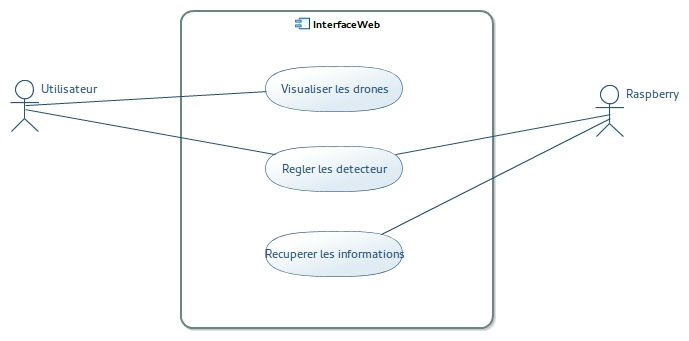
\includegraphics[width=\textwidth]{use_case}
  \caption{Cas d'utilisation de l'interface}
  \label{fig:use_case}
\end{figure}

\newpage
Ensuite, nous avons cherché a réaliser un diagramme de classe de notre interface. Pour cela nous avons défini 3 classes principales:

\begin{itemize}
\item index.php, qui réalise l'affichage dans un navigateur
\item serveur.py, qui récupère les données de chacun des radiogoniomètres
\item client.py, installé sur chaque radiogoniomètres il envoie les données des capteurs à travers un socket au serveur.
\end{itemize}

Le diagrammes de classe de la figure \ref{fig:class}, montre ce fonctionnement.

\begin{figure}[!h]
  \centering
  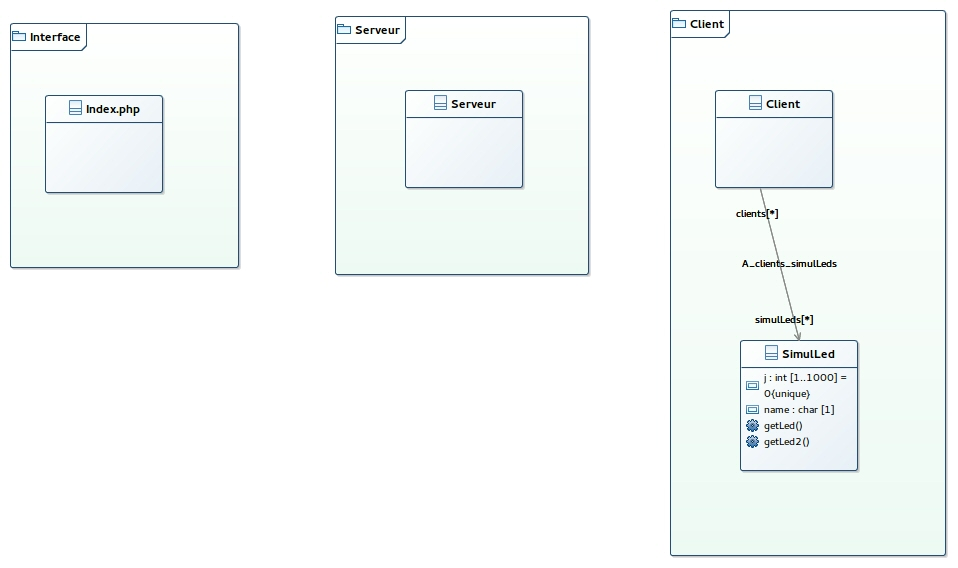
\includegraphics[width=\textwidth]{class_diagram}
  \caption{Diagramme de classe}
  \label{fig:class}
\end{figure}



\section{Conception}

\subsection{Client-Serveur}

Pour commencer nous avons cherché à donner une interface à nos \rpi pour communiquer avec l'ordinateur central, c'est l'interface Client/Serveur.
~\\

Cette interface a été codé en python. Nous avons choisi le python car c'est un langage souple et rapide. Nous avons réalisé la connection à l'aide d'un socket TCP/IP. De plus, le serveur se base sur du multi thread pour accepter plusieurs client. Le client se connecte donne, son identifiant puis sa communication est placé dans un thread. Ainsi, on a un serveur qui peut accepter une infinité de client.
~\\

Pour lancer le serveur il faut lancer le programme \textit{serveur.py} qui se met en écoute de client. Pour lancer le client il faut lancer le programme \textit{client.py}. Une illustration du terminal lors de l'exécution de ces commandes est donnée ci-dessous.
~\\

\begin{minipage}[h]{0.45\linewidth}

\begin{lstlisting}
./serveur.py
Serveur pret, en attente de requetes ...
Client RP1 connecte, adresse IP 127.0.0.1, port 51632.
RP1> led21
donc la direction 200
[...]
Client RP1 deconnecte.
[...]
Fin du serveur
\end{lstlisting}  
\end{minipage}\hfill
\begin{minipage}[h]{0.45\linewidth}
  
\begin{lstlisting}
./client.py
Connexion etablie avec le serveur.
Vous etes connecte. Envoyez vos messages.
la led allume: led21
[...]
Connexion interrompue.
\end{lstlisting}

\end{minipage}

~\\

On peut constater que la seule donnée que le \rpi envoie en continue est le numéro de la led qui s'est allumé. En effet, le modèle du Montréal 3v2 affiche le gisement sur un cadrant de 36 led. Dans notre solution nous avons décidé de garder ce cadrant et de placer le \rpi en parallèle du circuit pour détecter laquelle led s'est allumé. De plus, nous avons décidé de réaliser la conversion led/gisement au niveau du serveur pour des questions de modularités. 

~\\

Une foi les données reçut par le serveur, celui-ci les écrit dans un fichier qui s'appelle \textit{position}.



\subsection{Web}

Ensuite, nous nous sommes penché sur notre page web. Cette page web doit permettre à notre utilisateur de visualiser en temps réel la position du drone dans notre maillage. Pour cela nous avons fait le choix d'utiliser des solutions dynamiques tel que PHP, Javascript et JQuery.
~\\

Pour nous faciliter dans la réalisation du schéma modélisant notre treillis, nous avons choisi SVG. En effet, SVG nous permet de réaliser notre schéma de manière vectorielle. C'est-à-dire que l'on peut donner avec précision la position des capteurs ainsi que de leur droite de détection, mais surtout on peut rendre cela dynamique.
~\\

Le script ouvre le fichier \textit{position} qui a été précédemment rempli, et ajoute les points qui sont inscrit dans le fichier avec leur droite de détection. Mais cela ne suffit pas. En effet, si l'on s'arrête là on n'a qu'une position visible par un être humain il reste encore à la positionner. Pour cela nous utiliserons la triangulation (voir à la page \ref{sec:trian}).
~\\

Enfin, nous affichons de manière classé l'ensemble des \rpi qui été présent dans le fichier position à la droite de l'écran.




\subsection{Triangulation}
\label{sec:trian}
Les différents radiogoniomètres nous donnant un gisement de la détection, nous pouvons donc
réaliser une triangulation de la position du drone lorsqu’un nombre suffisant d’antenne détecte le
drone. Bien qu’une première estimation de la position peut-être obtenu à partir de deux drones,
nous considérons que le drone doit être détecté par au moins quatre senseurs pour que la position
soit acceptable.
~\\

Cependant, avant de pouvoir réaliser toute triangulation, l’acquisition des points d’intersection entre
les droites de détection issue du gisement fourni par les différents radiogoniomètres est nécessaire.
Pour se faire, à partir des angles, nous formulons une équation de droite plan, passant par les
radiogoniomètres respectifs, et tentons de trouver une solution à chaque système composé de deux
droites.
~\\

\begin{wrapfigure}{r}{0.5\textwidth}

  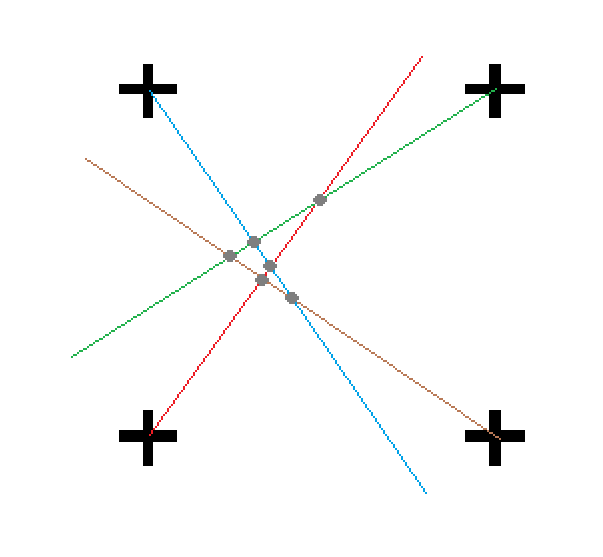
\includegraphics[width=0.5\textwidth]{triangulation1}
  \caption{triangulation}
\end{wrapfigure}

  Suite à la résolution de ces différents systèmes, nous
obtenons une liste de différentes solutions, solutions ici
schématisé avec des points de couleur grise. Nous observons
que, du fait de la portée de détection, ainsi que la géométrie
de notre treillis, certains points sont incohérents ou très
imprécis.

~\\
Notre première approche fut donc de positionner le drone à
la moyenne de l’ensemble des positions solutions d’un des
systèmes précédent. Cependant, après simulation, il s’est
avéré que, de par l’imprécision relative des
radiogoniomètres (les angles sont donnée à 5\up{o} près), la moyenne de donnait qu’une idée toute relative de la position du drone et souvent loin de la vérité, et
cela à cause d’intersections multiples entre les droites de détection.
Pour corriger cela nous avons fait le choix d’utiliser la médiane afin de supprimer tous les résultats
incohérents. A partir de la médiane des résultats, nous appliquons un gabarit circulaire et retenons
tous les points d’intersection compris dans ce gabarit. Une moyenne est alors appliquée à l’ensemble
de ces résultats nous permettant d’obtenir un résultat plus cohérent et moins sensible aux erreurs.


~\\
\newpage
Au final, nous obtenons la page web suivante:

\begin{figure}[!h]
  \centering
  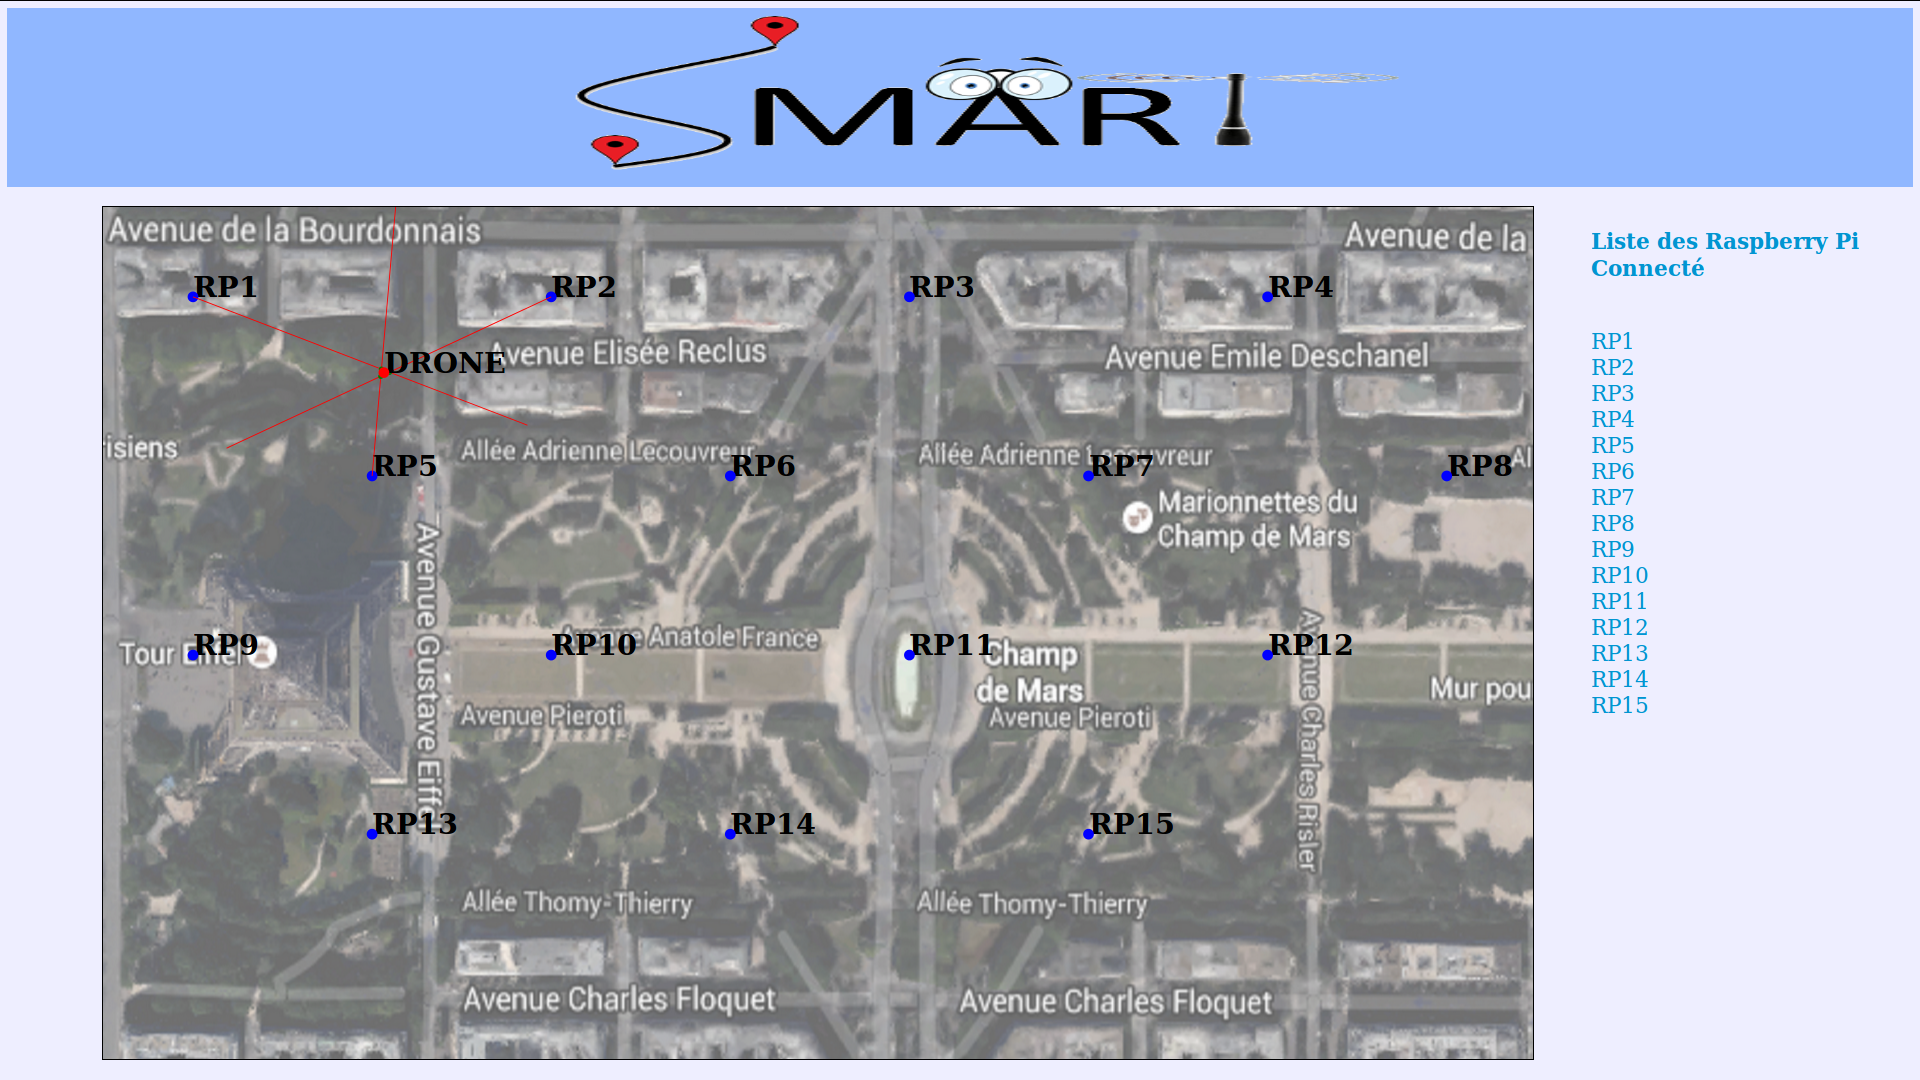
\includegraphics[width=\textwidth]{interface}
  \caption{Interface Web}
  \label{fig:interface}
\end{figure}





%%% Local Variables: 
%%% mode: latex
%%% TeX-master: "../rapport"
%%% End: 

\chapter{Réalisation}

%%% Local Variables: 
%%% mode: latex
%%% TeX-master: "../rapport"
%%% End: 

\part{Organisation d'équipe}


\chapter{Organisation du travail}


 \section{Méthode de travail}




% Nous avons cherché au mieux à répartir notre travail. Pour cela nous avons défini 3 grands axes de travail à l'issue de cette étude fonctionnelle.
% \begin{itemize}
% \item Réaliser les tests unitaires
% \item Dans un deuxième temps nous étudierons la phase de réalisation.
% \item Enfin nous testerons notre projet dans des conditions réelles.
% \end{itemize}
% ~\\

% Tout au long de ce projet nous avons choisi de réaliser notre travail en divisant notre équipe en 3 groupes de travail distincts formés respectivement de D'Acremont - Legay, Cotten - Rigaud, et Kenaan - Shehade. Notamment lors de l'état de l'art, ces groupes vont réaliser des recherches par binômes pour ensuite redistribuer les informations grâce aux outils mis à notre disposition (nous avons détaillé ces outils plus loin).
% ~\\

% De plus, nous avons décidé lors de la phase de conception de diviser ce travail en plusieurs sous ensembles que nous définirons plus tard et qui seront chacun d'eux testés indépendamment, à l'image de tests unitaires en programmation.



\section{Outils utilisés}

Au début de notre projet nous avons choisi d'utiliser plusieurs outils de travail en collaboration.

\begin{itemize}
\item Nous utilisons \LaTeX~pour la rédaction de nos rapports.
\item Nous avons hébergé notre projet sur GitHub. Cela nous permet de travailler de manière collaborative avec un versionning.
\item Enfin nous utilisons un Framaboard du groupe Framasoft pour gérer les taches de notre projet.
\end{itemize}

~\\
~\\

\subsection{Framaboard}
\begin{center}
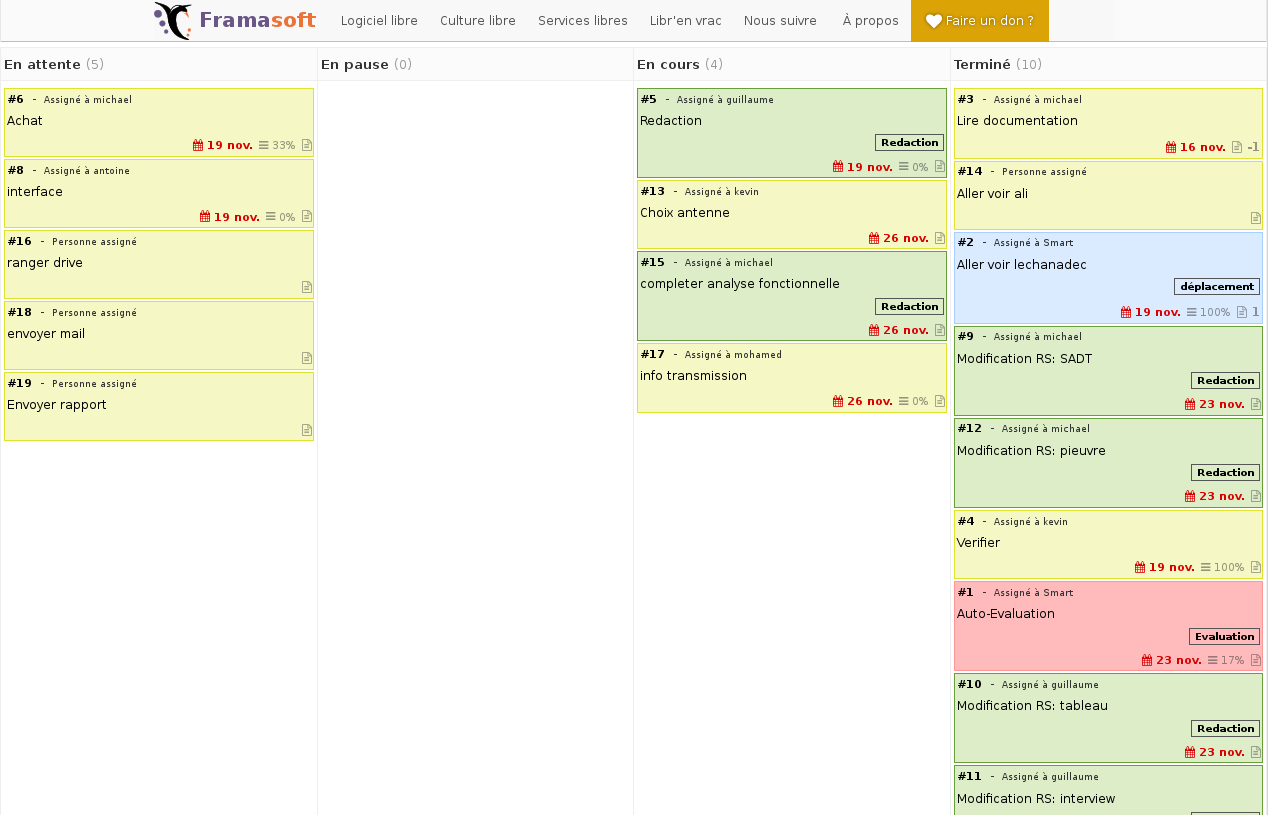
\includegraphics[width=0.9\textwidth]{framaboard}
\captionof{figure}{Impression d'écran de notre Framaboard}
\end{center}
Il est possible d'avoir accès en lecture à notre page Framaboard en cliquant  \textit{\href{https://smart.framaboard.org/?controller=board&action=readonly&token=ab1e20bb26472df067dc24cbd84d9b28eea71bfd68bdea07ab5a9b555ce0}{ici}}

\subsection{GitHub}
\begin{center}
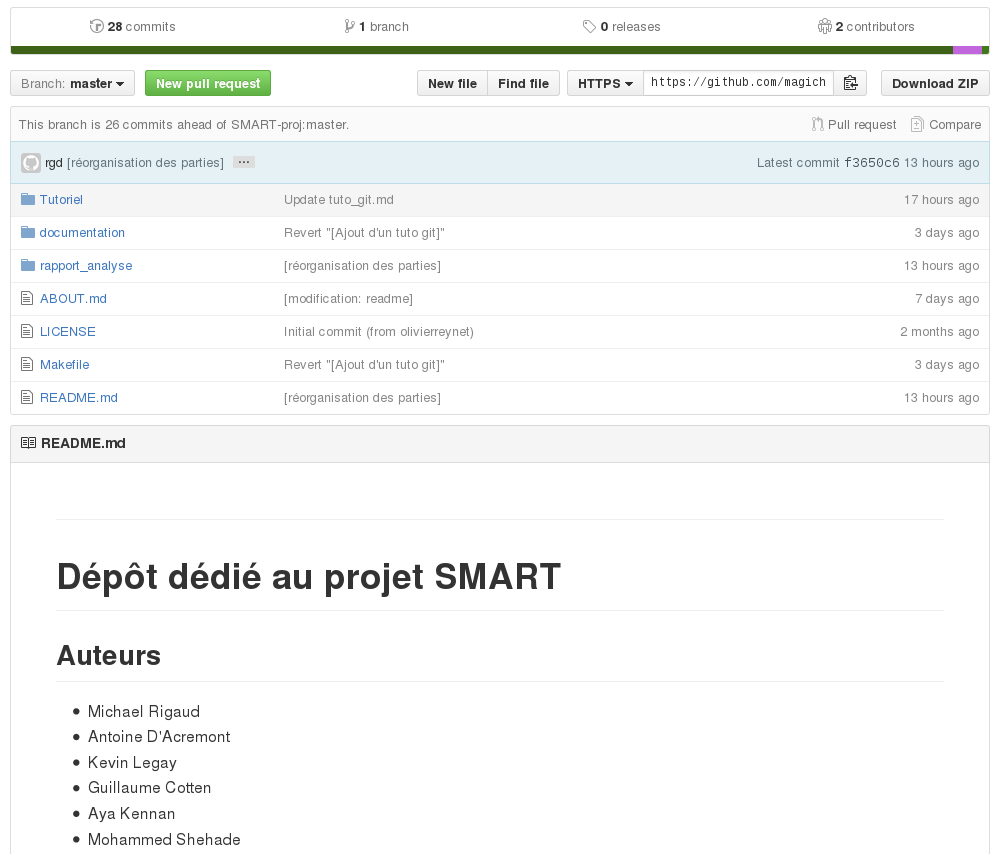
\includegraphics[width=0.9\textwidth]{github.png}
\captionof{figure}{Impression d'écran de notre GitHub}
\end{center}
Il est possible d'avoir accès à notre page GitHub en cliquant  \textit{\href{https://github.com/magichal/SMART}{ici}}






\section{Diagramme de Grant}

Le logiciel que nous avons utilisé durant notre projet permet de réaliser des TODO List, mais également d'afficher les taches enregistrées à travers un diagramme de Grant.

Nous avons au début du semestre 4 réalisé un diagramme de Grant de Prévision des taches principales à réaliser (figure \ref{fig:grant_pre}).

\begin{figure}[h]
  \centering
  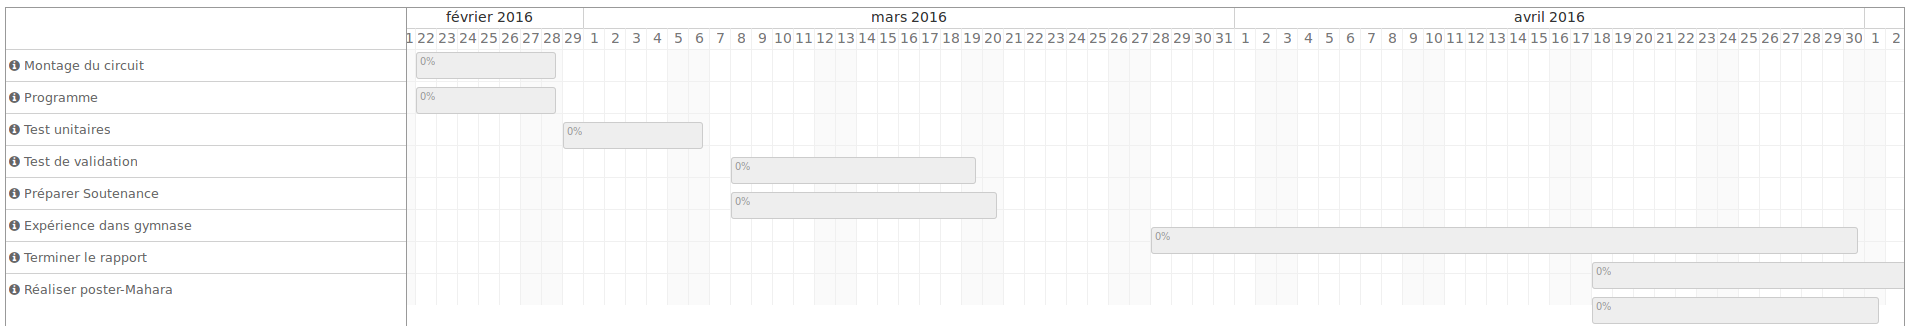
\includegraphics[width=\textwidth]{grant_prevision}
  \caption{Diagramme de Grant des prévision}
  \label{fig:grant_pre}
\end{figure}


A la fin du semestre nous obtenons le diagramme  \ref{fig:grant_fev}.
\begin{figure}[h]
  \centering
  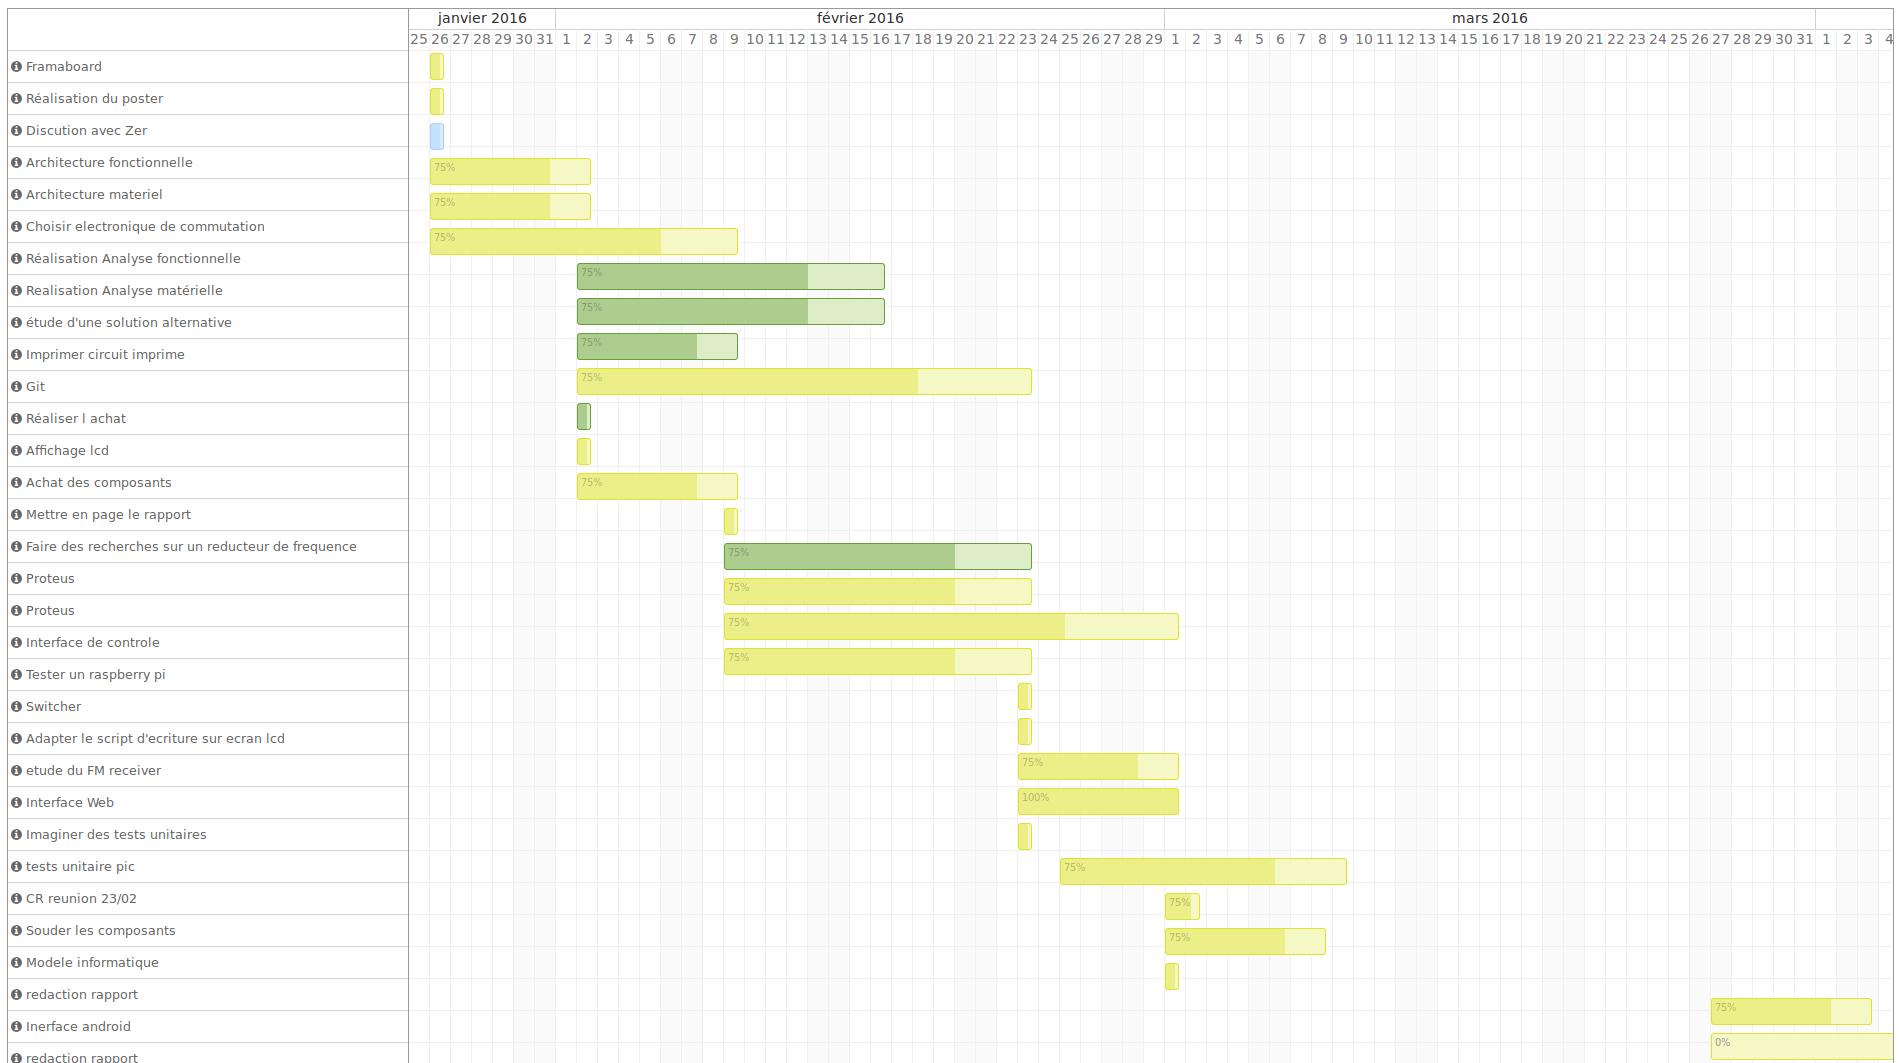
\includegraphics[width=\textwidth]{grant_fev}
  \caption{Diagramme de Grant (1)}
  \label{fig:grant_fev}
\end{figure}
\begin{figure}[h]
  \centering
  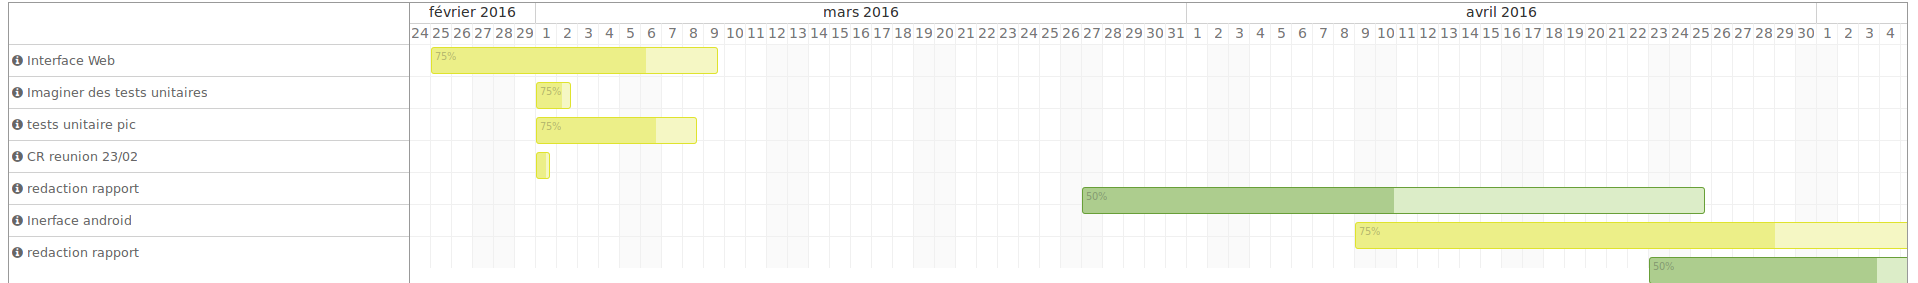
\includegraphics[width=\textwidth]{grant_mars}
  \caption{Diagramme de Grant (2)}
  \label{fig:grant_mars}
\end{figure}

~\\
Il est possible de constater qu'il y a une certaine chute d'activités au mois de mars. Une explication sera donnée dans le chapitre suivant.

De plus, on peut constater que certain objectifs n'ont pas été tenu. En effet, nous espérions pouvoir réaliser des tests de fonctionnement des le mois de mars, or a cause de retards de livraison nous n'avons pas pu réaliser un modèle testable. A cause de ces difficultés\footnote{Elles seront détaillés au chapitre \ref{chap:difficulte}} nous avons du repenser notre projet et nos prévisions ce qui a entraîné du retard dans notre travail.


%%% Local Variables: 
%%% mode: latex
%%% TeX-master: "../rapport"
%%% End: 


\chapter{Difficultés rencontrées}
\label{chap:difficulte}

Durant ce semestre, de nombreux obstacles à la réalisation de notre projet ont été rencontré. Ces difficultés sont de sources et de natures différentes, et ont conduit à une évolution des attentes et des objectifs de l’équipe pour atteindre le résultat actuel.~\\

Les premières difficultés sont de natures académiques et intellectuelles. En effet, nous avions pour objectif de réaliser notre propre radio-goniomètre à effet Doppler, couvrant le 2.4 GHz ambition réalisable mais complexe dans le temps imparti. La réalisation d’un tel système implique une solide maitrise en électronique et théorie des ondes, qualité que nous aurions pu acquérir avec plus de délais. De l’implémentation numérique de composants absents du logiciel Proteus, en passant par la réalisation du schéma électrique puis du circuit imprimé, nos notions en électroniques étaient trop sommaires pour se lancer dans une telle réalisation. Cela demeurait cependant la seule solution pour obtenir un système complet en fin d’année, le prix d’un tel radio-goniomètre avoisinant les 2000\euro ~sur le marché. 
La complexité de ce système a été accentuée par des retards de livraisons et de commande. Si certains de ces retards sont entièrement dus à notre innocence dans la conduite d’un projet, d’autres incombent uniquement aux fournisseurs. En effet, la commande de nos antennes accuse plus d’un mois de retard et devrait donc être annulé. Le dialogue avec le fournisseur n’y changeant rien, ce retard nous a d’autant plus conduit à faire évoluer nos attentes et nous recentrer sur la deuxième partie de notre projet, la gestion de la détection. D’une détection réelle, nous avons donc pris la décision de présenter une détection simulée, décision approuvée lors de la soutenance intermédiaire. 
~\\

Dans un second temps, les difficultés furent de natures humaines et relationnelles. Chaque groupe possède son élément moteur. Or, suite à des problèmes de santé, Michael RIGAUD a dû se retirer temporairement du groupe suite à sa période de convalescence. Cette période, démarrant en même temps que nos évolutions d’objectifs, a donc vu notre productivité et notre motivation diminuer à cause du retard accumulé sur la réalisation des goniomètres pour au final en abandonner la réalisation. Cette période aurait à l’inverse dû être un second départ pour l’ensemble du groupe afin de se relancer. 
Toutes ces difficultés rencontrées nous auront ouvert les yeux sur les obstacles à la réalisation d’un projet, obstacles auxquels nous pourront dorénavant nous préparer à l’avenir.


%%% Local Variables: 
%%% mode: latex
%%% TeX-master: "../rapport"
%%% End: 



%%%% CONCLUSION %%%%%%%%%

\chapter*{Conclusion}
\addcontentsline{toc}{chapter}{Conclusion}
\newpage

%%%% ANNEXE %%%%%%%%%%%%


\chapter*{Remerciments}
\addcontentsline{toc}{chapter}{Remerciements}

Avant de commencer la présentation de notre travail, nous profitons de l’occasion pour adresser nos remerciements à toutes les personnes qui ont contribué de près ou de loin à la réalisation de ce projet.

Nous tenons à exprimer nos vifs remerciements pour notre respectueux professeur, M. Mansour Ali, d’avoir accepté de nous encadrer, suivre notre travail, nous diriger, afin que nous puissions mener ce projet à terme, ainsi que pour son soutien, ses remarques pertinentes et son encouragement.

Nos remerciements vont aussi à M. Le Chenadec Gilles , qui nous a accompagné de près durant tout ce travail, pour sa disponibilité, pour la confiance qu’il a su nous accorder et les conseils précieux qu’il nous a prodigués tout au long de la réalisation de ce projet.

Nos remerciements vont aussi à tous les professeurs, enseignants et toutes les personnes qui nous ont soutenus jusqu’au bout, et qui n’ont pas cessé de nous donner des conseils très importants en signe de reconnaissance. Nous souhaitons que le travail réalisé soit à la hauteur de leurs espérances ainsi qu’aux attentes de notre encadrant.


\begin{figure}[!h]
  \centering
  
\includegraphics[width=0.3\textwidth]{merci}
\end{figure}

%%% Local Variables: 
%%% mode: latex
%%% TeX-master: "../rapport"
%%% End: 


\part*{Annexe}
\addcontentsline{toc}{part}{Annexe}
\appendix
\nocite{*}
%
\chapter{Drone}

\section{Définition}
La définition suivante est extraite de futura science \cite{futura}.~\\

Un drone est un aéronef sans passager ni pilote qui peut voler de façon autonome ou être contrôlé à distance depuis le sol. Le mot « drone » est employé pour désigner des véhicules aériens, terrestres, de surface ou sous-marins, alors que la classification anglo-saxonne distingue chaque type d’appareil.  ~\\

La taille d’un drone aérien peut aller de quelques centimètres pour les modèles miniatures à plusieurs mètres pour les drones spécialisés (surveillance, renseignement, combat, transport, loisirs). L’autonomie en vol va de quelques minutes à plus de 40 heures pour les drones de longue endurance.  

\section{Type des drones}

On distingue deux types des drones selon leur utilisation et leur taille : militaires et civiles. 

\subsection{Les drones militaires}

Le concept du drone a émergé durant la Premier Guerre mondiale. À l’origine, le drone était un avion-cible à vocation militaire. Son développement a suivi le rythme des grands conflits du XXe siècle : Seconde Guerre mondiale, guerre de Corée, du Vietnam, guerre froide, conflits au Moyen-Orient, guerre d’Irak, d’Afghanistan ou encore en ex-Yougoslavie. Les drones sont plus économiques tout en évitant de mettre en jeu la vie des pilotes et de déployer des troupes terrestres notamment pour les missions de reconnaissance, de surveillance et les attaques ciblées. Leur utilisation au sein des armées et forces de police est devenue prépondérante.  ~\\

% \subsubsection{Types des missions}

 
%En effet, 
Les missions qui leur sont dévolues sont très variées:  ~\\

\begin{itemize}
\item[1.] Écoute des signaux électromagnétiques.
\item[2.]    Observation et surveillance. 
\item[3.]    Détection de missile balistique grâce à une alerte avancée. 
\item[4.]    Relais de communication. 
\item[5.]    Illumination de cibles. 
\item[6.]    Brouillage. 
\item[7.]     Et pour certains, bombardement. 
%\item[8.] Transport de marchandise.
\end{itemize}
 

\subsection{Les drones civils }

Dans le civil, de nombreux domaines (cinéma, télévision, agriculture, environnement, etc.) ont vu les drones susciter des applications inédites grâce à leur capacité à embarquer des appareils photo, des caméras, des caméras infrarouge ou des capteurs environnementaux. Plusieurs sociétés spécialisées dans le transport (DHL, UPS, Allship, La Poste) ainsi que le géant du e-commerce Amazon travaillent sur des concepts de drones-livreurs. Ce type de service a été introduit en 2015 aux Émirats arabes unis pour la livraison de documents officiels.  ~\\

Les drones de loisir ont connu un essor important à partir des années 2010 avec l’arrivée d’appareils miniaturisés, abordables et suffisamment maniables pour être accessibles aux novices. En France, l'utilisation des drones est réglementée par le Code de l’aviation civile, le Code des transports et deux arrêtés émis en 2012. 

%[1]: http://www.futura-sciences.com/magazines/espace/infos/dico/d/aeronautique-drone-6174/ 


    

\section{Fréquence}

Il y a 3 fréquences utilisées pour la communication entre le drone et le télécommande: ~\\
\begin{itemize}
\item 1,3 GHz
\item    2,4 GHz 
\item    5,8 GHz 
\end{itemize}  
~\\


Pour une meilleure qualité d’image, mieux vaut utiliser la bande de 5,8 GHz sachant que le 2,4 GHz permet de plus longues distances mais une qualité d’images plus faible. 

Afin d’éviter les interférences, mieux vaut éviter d’émettre sur la même bande que votre radiocommande. 

Le 2,4 GHz est la même bande que le Wifi, donc à éviter en milieu urbain et en cas d’utilisation évitez d’allumer votre smartphone à côté. 

\section{Types de modulations }

Mais il est impossible d’envoyer un signal numérique tel quel par ondes électromagnétiques. Le signal a besoin d’être modulé, c'est-à-dire transformé d’un signal numérique à un signal analogique. L’opération inverse, la démodulation, se fait par la suite après la réception du signal par la station afin d’obtenir une information exploitable. 

 
\begin{figure}[h]
  \centering
  \includegraphics[width=0.7\textwidth]{modulation}
  \caption{types de modulations}
\end{figure}
 


Il existe plusieurs types de modulation dont voici les plus connus: ~\\

 
\textit{AM (Amplitude Modulation) :} Pour faire passer de l’information, on modifie l’amplitude du signal au cours du temps. ~\\

 

\textit{FM (Frequency Modulation) :} Pour faire passer de l’information on modifie la fréquence du signal au cours du temps. ~\\

 

\textit{PM (Phase Modulation) :} C’est la technologie la plus utilisés pour les transmissions radio. Ici on fait passer l’information en modifiant la phase du signal. L’amplitude et la fréquence du signal restent donc fixes. Il existe plusieurs types de modulations par phases : BPSK \footnote{Binary Phase Shift keying}, QPSK\footnote{Quadratic PSK} … BPSK est binaire, on peut donc utiliser deux phases différentes et ainsi faire passer deux types d’informations (0 ou 1). QPSK est quadratique c'est-à-dire que l’on peut utiliser quatre phases différentes donc que l’on peut transmettre quatre types d’informations (00, 01, 10,11). Plus le nombre de phases augmente plus le nombre d’informations pouvant être véhiculé augmente. Mais cela rend le signal plus  exposé aux erreurs car les phases sont de plus en plus proches. ~\\

 

Lorsque l’on modifie la phase d’un signal, on « décale » le signal dans le temps. Graphiquement, cela se traduit par une translation de la courbe du signal sur l’axe des abscisses. La modulation de phase s’exprime en degrés ou en radians. Ainsi 360\up{0} (ou 2n radians) correspond à un décalage d’une période. On dit de deux signaux qu’ils sont en phase lorsqu’ils se superposent. 

 

\begin{figure}[h]
  \centering
  \includegraphics[width=0.7\textwidth]{signal}
  \caption{Exemple d'un signal modulé en phase avec un changement de phase de 180\up{0}}
\end{figure}

 

 

Une fois que ce signal modulé arrive à destination, on opère l’action inverse : la démodulation. Cela permet d’avoir une information numérique exploitable et d’ensuite pouvoir afficher l’image sur un écran afin que le pilote puisse voir ce que drone \og voit \fg{}. 

 

La transmission de données par ondes électromagnétiques ne se fait pas sans erreur, surtout lorsque celles-ci traversent plusieurs milliers de kilomètres dont l'atmosphère terrestre. Ces erreurs surviennent cependant en groupe et de façon très localisé. Mais de simples algorithmes de correction d’erreur comme le FEC\footnote{Forward Error Correction} peuvent assurer de bonnes conditions de transmissions. 

\section{Législations}



La législation en France impose une puissance d’émission maximale de 25 mW dans la fréquence des 5.8 GHz et 100 mW dans la fréquence 2.4 GHz. ~\\

Pour voler en immersion, il faut être 2 avec 2 radiocommandes, un \og esclave\fg{} et un \og maître\fg{} pouvant reprendre le contrôle à tout moment si besoin. ~\\

Les agents de contrôle peuvent, à tout moment, effectuer des contrôles, tant au niveau des utilisateurs amateurs que professionnels, sur le respect des caractéristiques techniques radios des drones. Une utilisation du spectre est trop dangereuse. En cas de non-respect de celles-ci, le matériel peut être saisi et un procès-verbal dressé.~\\ 

Cependant, un arrêté sur les conditions d’utilisation et des personnes capables de  piloter ces drones a été rédigé en France par les services de l’aviation civile le 10 Décembre 2009. Dans l’article 3, les drones doivent être connus des services de l’aviation civile lorsque les drones ne sont pas pour des activités sportives ou récréatives. Ils doivent être connus lorsqu’ils font partie d’une association d’aéromodélisme mais aussi lorsqu’ils évoluent à plus de 150 mètres d’altitudes (ils doivent fournir des justificatifs prouvant le besoin et disposer de précautions particulières, et surtout les vols de nuit ne sont pas autorisés. ~\\

L’utilisation de drones civils est très contraignante. En effet, l’utilisateur doit de demander une autorisation au service de l’aviation civile, pour chaque vol, plusieurs semaines à l’avance ce qui est presque impossible, car les drones dépendent de la météo. De plus, aucune autorisation n’est délivrée à l’heure actuelle pour des survols avec des drones civils dans des zones civiles de zones habitées ou avec un rassemblement de personnes (manifestation). Or, c’est dans ces zones que sont prises la majeure partie des photographies. Il est faux de croire qu’en dessous de 150 mètres d’altitudes il n’y a pas de règlementation et que les avions et hélicoptères avec pilote ne peuvent pas descendre à cette altitude. A cette altitude, il est nécessaire de posséder une autorisation, car sur le territoire français des milliers d’heures de vols se font entre 50 et 150 mètres d’altitudes avec des avions et hélicoptères traditionnels (vols basse altitude d’entrainements militaires, interventions d’hélicoptères de secours).  Les aéronefs traditionnels  ne peuvent pas éviter les drones à cette altitude à cause de leur faible taille, presque invisible en vol. 



%%% Local Variables: 
%%% mode: latex
%%% TeX-master: "rapport_analyse"
%%% End: 

%
\chapter{Organisation du travail}


\section{Méthode de travail}

Nous avons cherché au mieux à répartir notre travail. Pour cela nous avons défini 3 grands axes de travail à l'issue de cette étude fonctionnelle.
\begin{itemize}
\item Dans un premier temps nous allons réaliser l'état de l'art.
\item Dans un deuxième temps nous étudierons la phase de réalisation.
\item Enfin nous testerons notre projet dans des conditions réelles.
\end{itemize}
~\\

Tout au long de ce projet nous avons choisi de réaliser notre travail en divisant notre équipe en 3 groupes de travail distincts formés respectivement de D'Acremont - Cotten, Legay - Rigaud, et Kenaan - Shehade. Notamment lors de l'état de l'art, ces groupes vont réaliser des recherches par binômes pour ensuite redistribuer les informations grâce aux outils mis à notre disposition (nous avons détaillé ces outils plus loin).
~\\

De plus, nous avons décidé lors de la phase de conception de diviser ce travail en plusieurs sous ensembles que nous définirons plus tard et qui seront chacun d'eux testés indépendamment, à l'image de tests unitaires en programmation.



\section{Outils utilisés}

Lors de notre projet nous avons choisi d'utiliser plusieurs outils de travail en collaboration.

\begin{itemize}
\item Nous utilisons Office 365. Nous avons créé un groupe de travail où nous partageons des fichiers et envoyons des mails de manière centralisée.
\item Nous utilisons également \LaTeX~pour la rédaction de nos rapports.
\item Nous pensons finalement utiliser Git et GitHub lors de notre phase de conception. Nous avons pour cela crée un projet sur GitHub.
\item Après plusieurs difficultés, nous avons réussi à utiliser Framaboard du groupe Framasoft pour gérer notre projet.
\end{itemize}

~\\
~\\

\subsection{Framaboard}
\begin{center}
\includegraphics[width=0.9\textwidth]{framaboard}
\captionof{figure}{Impression d'écran de notre Framaboard}
\end{center}
Il est possible d'avoir accès en lecture à notre page Framaboard en cliquant  \textit{\href{https://smart.framaboard.org/?controller=board&action=readonly&token=ab1e20bb26472df067dc24cbd84d9b28eea71bfd68bdea07ab5a9b555ce0}{ici}}

\subsection{GitHub}
\begin{center}
\includegraphics[width=0.9\textwidth]{github}
\captionof{figure}{Impression d'écran de notre GitHub}
\end{center}
Il est possible d'avoir accès à notre page GitHub en cliquant  \textit{\href{https://github.com/magichal/SMART}{ici}}






  


%%% Local Variables: 
%%% mode: latex
%%% TeX-master: "rapport_analyse"
%%% End: 

%\chapter{Correspondance}
\label{chap:mail}


\includepdf[pages={1,2}]{./images/mail.pdf}


%%% Local Variables: 
%%% mode: latex
%%% TeX-master: "../../rapport"
%%% End: 


\chapter{Validation Fonctionnel Usine}


%%% Local Variables: 
%%% mode: latex
%%% TeX-master: "../rapport"
%%% End: 
\chapter{Validation Fonctions de Service}


\begin{tabular}{|p{0.2\textwidth}| |p{0.2\textwidth}  |m{0.22\textwidth}  |p{0.22\textwidth} |}	

     \hline
     Numéro & Désignation & État & Commentaires \\ \hline
     FS1 & Détecter des drones à portée de réception par les antennes dans un domaine de fréquence prédéfini & Non validé & L'absence de capteur fonctionnel ne permet pas de valider entièrement cette fonction \\ \hline
     FS2a & Retourner la position du drone à l'utilisateur en temps réel & Partiellement validé & La position est transmise en temps réel uniquement dans le cadre des simulations \\ \hline
     FS2b & Avoir une précision de l'ordre du mètre & Non validé & Capteur non fonctionnel, impossible de vérifier la précision exacte \\ \hline
     FS3 & Suivre les déplacements du drone en temps réel & Partiellement validé & Le système suis bien les drones simulés \\ \hline
     FS4a & Alerter l'utilisateur en cas de nouvelle détection par un message via un PC & Validé & Possible via l'interface web \\ \hline
     \hline
   \end{tabular}

\begin{tabular}{|p{0.2\textwidth}| |p{0.2\textwidth}  |m{0.22\textwidth}  |p{0.22\textwidth} |}	

	\hline
	Numéro & Désignation & État & Commentaires \\ \hline
   	FS4b & Alerter l'utilisateur en cas de nouvelle détection via l'application Android & Validé & Dans le cas ou le drone est détecté l'utilisateur est bien averti \\ \hline
   	FS5 & Analyser et retourner la vitesse de déplacement du drone & Non validé & Pas de capteur fonctionnel pour tester cette fonction \\ \hline
   	FS6 & Retourner la trajectoire du drone à l'utilisateur & Validé & Via l'interface web \\      
   	\hline
\end{tabular}
	
%%	\hline
%%	Numéro & Désignation & État & Commentaires  \hline
%%	FS1 & Détecter des drones à portée de réception par les antennes dans un domaine de fréquence prédéfini & Non validé & L'absence de capteur fonctionnel ne permet pas de valider entièrement cette fonction  \hline
	


%%% Local Variables: 
%%% mode: latex
%%% TeX-master: "../rapport"
%%% End: 
\chapter{Tests Unitaires}


\begin{tabular}{|p{0.3\textwidth}  |m{0.3\textwidth}  |p{0.3\textwidth} |}	
\hline
Test & État & Commentaires \\ \hline
\multicolumn{3}{|c|}{PIC}\\ \hline
PIC16F628A & Échec & Réaction partielle du PIC aux entrées. Un autre protocole est nécéssaire \\ \hline
PIC12F675 & Échec & Réaction partielle du PIC aux entrées. Un autre protocole est nécéssaire \\ \hline
PIC18F4520 & Échec & Réaction partielle du PIC aux entrées. Un autre protocole est nécéssaire \\ 
\hline
\multicolumn{3}{|c|}{Plaques et pistes}\\ 
\hline
Test des pistes de la carte principale & Réussite & Test au multimètre. Passage courant OK, tension OK et faible résistance des pistes \\ 
\hline
Test des pistes de la carte d'affichage & Réussite & Test au multimètre. Passage courant OK, tension OK et faible résistance des pistes \\
\hline
\multicolumn{3}{|c|}{Filtre passe-bande}\\ 
\hline
Bande passante & Réussite & Amplitude Max à 2.45GHz, faible atténuation pour f>2.5GHz \\
\hline
Coefficient de réflexion & Réussite & S11 faible sur la bande passante \\
\hline
Coefficient de transmission & Réussite & log(S21) proche de 2dBm \\
\hline
\multicolumn{3}{|c|}{VCO}\\ \hline
Fréquence libre & Réussite & Mesure à 1.35GHz proche de la valeur constructeur \\ 
\hline
Tension efficace & Réussite & Tension idéale : 8V \\
\hline
Sortie VCO avec régulateur & Réussite & Fréquence de sortie 1.91GHz \\
\hline
\multicolumn{3}{|c|}{Down-converter}\\ \hline
Fréquence de sortie & Reporté & A reprogrammer \\
\hline
\end{tabular}

\begin{tabular}{|p{0.3\textwidth}  |m{0.3\textwidth}  |p{0.3\textwidth} |}	
\hline
\multicolumn{3}{|c|}{Raspberry}\\ \hline
Test d'allumage & Réussite & Fonctionne parfaitement sur alimentation secteur \\
\hline
Test Raspbian & Réussite & Installation et test des fonctionnalités python de Raspbian \\ 
\hline
Test GPIO & Réussite & Les ports GPIO choisis pour le projet fonctionnent dans les 2 sens \\
\hline
Test Client Raspberry & Réussite & Connection et communication avec le serveur (Ordinateur Michael) en local et en externe \\
\hline
\multicolumn{3}{|c|}{Application Android}\\ \hline
Lancement de l'application & Réussite & Testée sur 3 appareils différents \\
\hline
Communication avec le serveur & Réussite & Échange de messages simples dans les deux sens \\
\hline

\end{tabular}

\chapter{Documentation Technique du Raspberry Pi B+}
\label{annexe:rpi}

\section{Définition}


\textit{\og Le Raspberry Pi est un nano-ordinateur monocarte à processeur ARM conçu par le créateur de jeux vidéo David Braben, dans le cadre de sa fondation Raspberry Pi.}

\textit{Cet ordinateur, qui a la taille d'une carte de crédit, est destiné à encourager l'apprentissage de la programmation informatique2 ; il permet l'exécution de plusieurs variantes du système d'exploitation libre GNU/Linux et des logiciels compatibles. Il est fourni nu (carte mère seule, sans boîtier, alimentation, clavier, souris ni écran) dans l'objectif de diminuer les coûts et de permettre l'utilisation de matériel de récupération.}

\textit{Son prix de vente était estimé à 25 \$, soit 19,09 \euro, début mai 2011. Les premiers exemplaires ont été mis en vente le 29 février 2012 pour environ 25 \euro. Début 2015, plus de cinq millions de Raspberry Pi ont été vendus. De multiples versions ont été développées (voir la liste ci-dessous), on trouve les dernières à un peu plus de 25 \euro pour le B+, à un peu plus de 30 \euro pour le Pi 2 (2015) et à un peu plus de 45 \euro pour le Pi 3 (2016)\fg{}} Wikipédia \cite{wiki_rpi}

\section{Caractéristique et connectiques}
\begin{tabular}[c]{|l|l|}
\hline
\multicolumn{2}{|c|}{Caractéristiques}\\
\hline
Micro-contrôleur &	Broadcom BCM2835 ARM1176JZFS\\
Vitesse d'horloge& 	700 MHz\\
RAM &	512 Mo\\
\hline
\multicolumn{2}{c}{}\\
\hline
\multicolumn{2}{|c|}{Connectiques}\\
\hline
Port(s) USB &	4\\
Port Ethernet / RJ45 &	1\\
Connecteur(s) audio analogique &	1 sortie jack 3,5 mm\\
HDMI 	&1\\
Port pour carte mémoire 	&1 port micro SD\\
Alimentation &	via port micro USB 5V\\
\hline
\end{tabular}

\newpage
\section{Schéma technique}



\begin{figure}[!h]
  \centering
  \includegraphics[width=\textwidth]{raspberrypi_doc_mecanique}
  \caption{Dessin mecanique}
\end{figure}

\begin{figure}[!h]
  \centering
  \includegraphics[width=\textwidth]{raspberrypi_doc_schema}
  \caption{Schéma technique}
\end{figure}

%%% Local Variables: 
%%% mode: latex
%%% TeX-master: "../rapport"
%%% End: 


\chapter{Documentation Technique à Raspbian}
\label{annexe:raspbian}

Raspbian (recommended for Raspberry Pi 1) – is maintained independently of the Foundation; based on the Debian ARM hard-float (armhf) architecture port originally designed for ARMv7 and later processors (with Jazelle RCT/ThumbEE and VFPv3), compiled for the more limited ARMv6 instruction set of the Raspberry Pi 1. A minimum size of 4 GB SD card is required for the Raspbian images provided by the Raspberry Pi Foundation. There is a Pi Store for exchanging programs.

    The Raspbian Server Edition is a stripped version with fewer software packages bundled as compared to the usual desktop computer oriented Raspbian.

    The Wayland display server protocol enables efficient use of the GPU for hardware accelerated GUI drawing functions.[104] On 16 April 2014, a GUI shell for Weston called Maynard was released.

    PiBang Linux – is derived from Raspbian.

    Raspbian for Robots – is a fork of Raspbian for robotics projects with Lego, Grove, and Arduino.

%%% Local Variables: 
%%% mode: latex
%%% TeX-master: "../rapport"
%%% End: 


\chapter{Client.py}

\lstinputlisting[style=python]{../InterfaceWeb/Client/client.py}


%%% Local Variables: 
%%% mode: latex
%%% TeX-master: "../rapport"
%%% End: 


\chapter{Serveur.py}

\label{chap:serveur}

\lstinputlisting[style=python]{../InterfaceWeb/Serveur/serveur.py}


%%% Local Variables: 
%%% mode: latex
%%% TeX-master: "../rapport"
%%% End: 

\newpage
 \listoffigures
 \printindex
 \bibliographystyle{frplain}
  \bibliography{biblio}

\end{document}
%%%%%%%%%%%%%%%%% FIN DU DOCUMENT
